\documentclass[12pt, a4paper]{article}

\usepackage[T1]{fontenc}
\usepackage[utf8]{inputenc}
\usepackage[ngerman]{babel}
\usepackage{eurosym}
\usepackage{graphicx}
\usepackage{ifpdf}
%\usepackage{times}
\usepackage{longtable}
\usepackage{multicol}
\usepackage[figuresleft]{rotating} % Stundenplan im Anhang
\usepackage{enumitem} % Checkliste
\usepackage{qrcode} % Umschlagrückseite & Links
\usepackage{xcolor,colortbl}
\usepackage{tabularx}

% For hyperlinks
\ifpdf
	\usepackage{hyperref}
\else
	\usepackage[ps2pdf,breaklinks=true]{hyperref}
\fi

%
\pagestyle{plain}
% Einrückung der ersten Zeile eines Absatzes
\setlength{\parindent}{0mm}
% Abstand zwischen zwei Absätzen
\setlength{\parskip}{1em plus0.5ex minus0.5ex}
\setlength{\leftmargin}{0.0em}

\renewcommand*\descriptionlabel[1]{\hspace\labelsep
	\normalfont\bfseries #1}

%Serifenfrei
\renewcommand*\familydefault{\sfdefault}

\newcommand{\At}{@}


\hsize 15.5cm
\vsize 23cm
\hoffset-1cm
\voffset-2.2cm
\textheight=\vsize
\textwidth=\hsize

\newif\ifwintersemester
\newif\ifsommersemester

%set for info, unset for kogni
\newif\ifinfo


\begin{document}

\emergencystretch=2cm

%\font\cms=cmss17 scaled \magstep2
\font\vlarge=cmbx12 scaled \magstep5
\newdimen\oldbaselineskp
\newcount\auflage
\newcount\jahr
\newcount\jahrpluseins
\setcounter{secnumdepth}{0}

\newcommand*{\email}[1]{\url{#1}}
\newcommand*{\filename}[1]{\url{#1}}

%%%%%%%%%%%%%%%%%%%%%%%%%%%%%%%%%%%%%%%%%%%%%%%%%%%%%%%%%%%%%%%%%%%%%%%%%%%%%
%%% Auflage und Jahr hier eintragen
%%%%%%%%%%%%%%%%%%%%%%%%%%%%%%%%%%%%%%%%%%%%%%%%%%%%%%%%%%%%%%%%%%%%%%%%%%%%%

\input{makeconfig.tex}

% Semesterticket
\newcommand{\Ticketpreis}{\EUR{104,90}}

\ifinfo
	\newcommand{\Infoprof}{Grust}
	\newcommand{\Matheprof}{Ochs}

	% studentische Beratung
        \newcommand{\studBeratungInfo}{Elisabeth Fritze}
        \newcommand{\studBeratungMedien}{Vanessa Kirchner}
        \newcommand{\studBeratungMedizin}{Felix Sieghörtner}
        \newcommand{\studBeratungLehramt}{Saskia Honeck}
        \newcommand{\studBeratungKogni}{Lena Hoeppe \& Lia Schmid}

\newcommand{\Studiendekan}{Nieselt}
\else
	\newcommand{\studBeratung}{Lena Hoeppe und Lia Schmid}
	\newcommand{\studBeratungTwolines}{Lena Hoeppe und \newline Lia Schmid}
	\newcommand{\kognimentoren}{Fynn Neurath und Julia Dietl}
	\newcommand{\kognimentorenTwolines}{Fynn Neurath und \newline Julia Dietl}
\fi

% Shorthandles for QR-Codes
% small
\newcommand{\link}[2]{
	\colorbox{gray!10}{
		\parbox{\textwidth}{
			\begin{minipage}{0.2\textwidth}
				\qrcode{#1}
			\end{minipage} \hfill
			\begin{minipage}{0.8\textwidth}
				\textbf{#2} \\ #1
			\end{minipage}
}}}

% big
\newcommand{\linkbig}[3]{
	\colorbox{gray!10}{
		\parbox{0.5\textwidth}{
			\centering
			\qrcode{#1} \\
			\vspace*{2mm}
			\textbf{#2} \\ #1
	}}
	\hfill
	\parbox{0.5\textwidth}{
		#3
	}
}

% ========= Corona Disclaimer ===========
% Disclaimer with desciption parameter
\newcommand{\coronabox}[1]{
    \noindent
    \colorbox{orange!10}{
        \parbox{\textwidth}{
            \begin{minipage}{.15\textwidth}
                \centering
                \color{red}\Huge\faIcon{biohazard}
            \end{minipage}\begin{minipage}{.85\textwidth}
                \vspace*{3mm}
                \textbf{Corona Disclaimer}\\
                #1
                \vspace*{3mm}
            \end{minipage}
}}}

% Generic Disclaimer
% The text below is not final. Feel free to find something mor suitable
\newcommand{\corona}{\coronabox{
Wie bei allem lässt sich hier nichts definitiv sagen. Bitte informiere dich \\ direkt bei der betreffenden Stelle.
}}


%%%%%%%%%%%%%%%%%%%%%%%%%%%%%%%%%%%%%%%%%%%%%%%%%%%%%%%%%%%%%%%%%%%%%%%%%%%%%
\jahrpluseins=\jahr
\advance \jahrpluseins by 1

%%%% Seite 1
\ifinfo
	\begin{titlepage}
	\thispagestyle{empty}
	{\sf \number\auflage. Auf\/lage \hfill Tübingen, 
		\ifwintersemester
		Oktober \number\jahr}\\
	\fi
	\ifsommersemester
	April \number\jahr}\\
	\fi 
	\vspace*{2cm}
	%\rule[2mm]{\textwidth}{.2cm}\\
	
\includegraphics[width=\textwidth]{shared/logos/fsilogo_neu}
	%\rule{\textwidth}{0.2cm}\\
	
	\begin{center}
		\vspace*{1.5cm}
		\oldbaselineskp=\baselineskip
		\baselineskip 45pt
		
		\Huge Informationen für Erstsemester\\[2cm]
		
		\ifwintersemester
		Wintersemester \number\jahr /\number\jahrpluseins
		\fi
		\ifsommersemester
		Sommersemester \number\jahr
		\fi
		\\
		
		\baselineskip=\oldbaselineskp
		\vfill
		\textsc{Eberhard Karls \\ Universität Tübingen}
		%
\includegraphics[width=9cm]{shared/logos/unilogo_neu}
		%\uni H \rm ~~~ \raisebox{18pt}{\Huge Universität Tübingen}\\[2cm]
	\end{center}
	\eject
\end{titlepage}

\else
	\begin{titlepage}
	\thispagestyle{empty}
%	\vspace*{2cm}
	%\rule[2mm]{\textwidth}{.2cm}\\
	
\includegraphics[trim= 40 0 0 0,width=\textwidth]{kogni/logos/fsk_logo}
	%\rule{\textwidth}{0.2cm}\\
	{\sf \space\number\auflage. Auf\/lage \hfill Tübingen,
                \ifwintersemester
                Oktober \number\jahr}\\
        \fi
        \ifsommersemester
        April \number\jahr}\\
        \fi
 
	\begin{center}
		\vspace*{1.5cm}
		\oldbaselineskp=\baselineskip
		\baselineskip 45pt
		
		\Huge Informationen für Erstsemester\\[2cm]
		
		\ifwintersemester
		Wintersemester \number\jahr /\number\jahrpluseins
		\fi
		\ifsommersemester
		Sommersemester \number\jahr
		\fi
%		\\
		
		\baselineskip=\oldbaselineskp
		\vfill
		
\includegraphics[width=9cm]{kogni/logos/unilogo_neu}
		%\uni H \rm ~~~ \raisebox{18pt}{\Huge Universität Tübingen}\\[2cm]
	\end{center}
	\eject
\end{titlepage}

\fi

%%%% Seite 2
\ifinfo
	\thispagestyle{empty}

\textbf{Fachschaft Informatik:}\\
Informationen für Studienanfänger\\
% StudienanfängerInnen
%\number\auflage. erweiterte und bearbeitete Auf\/lage, Tübingen \number\jahr\\[1cm]
\number\auflage. komplett überarbeitete Auf\/lage, Tübingen \number\jahr\\[1cm]
\medskip \\

\begin{tabular}{ll}
	Redaktion & Alexander Goetz, Meret Häusler, Georgios Angelou \\ %TODO Hier die Leute reinschreiben die rumflamen
	Grafik & Tim Beckmann, Florian Heimgärtner \\
	Satz & \LaTeX
\end{tabular}\\

\vfill
%Mit freundlicher Unterstützung von Dr. Katja Nieselt und Claudia Walter \medskip \\
\begin{minipage}[c]{0.1\textwidth}
	
\includegraphics[width=\linewidth]{info/logos/by-nc.pdf}
\end{minipage}
\begin{minipage}[c]{0.9\textwidth}
	%TODO insert \link{}{}?
	Die verwendeten Comics stammen von Randall Munroe (\url{https://xkcd.com}) und stehen unter der \emph{Creative Commons Attribution-NonCommercial 2.5}-Lizenz.
\end{minipage}

\copyright 1994--\number\jahr ~by Fachschaft Informatik Tübingen\\

\medskip

\textbf{E-Mail:} \hfill
\email{fsi@fsi.uni-tuebingen.de}\\
\textbf{WWW:} \hfill
%TODO insert \link{}{}?
\url{https://www.fsi.uni-tuebingen.de/}
\newpage

\else
	\thispagestyle{empty}

\textbf{Fachschaft Kognitionswissenschaft:}\\
Informationen für Studienanfänger\\
% StudienanfängerInnen
\number\auflage. Auf\/lage, Tübingen \number\jahr\\[0.2cm]
% Zur besseren Einsicht, welche Version in Druck gegeben wurde und als Hinweis zum Ort des Sourcecodes
{\footnotesize Sourcecode verfügbar unter \url{https://github.com/fsi-tue/anfiheft}\\
               Aktuellste Version verfügbar unter \url{https://teri.fsi.uni-tuebingen.de/anfiheft/}\\
	       Revision: \gitCommit\\[1cm]}


\begin{tabular}{ll}
	Redaktion & Alexander Goetz, Linus Szillat und alle die vor uns waren\\ %TODO Hier die Leute reinschreiben die rumflamen
	Grafik & Tim Beckmann, Florian Heimgärtner \\
	Satz & \LaTeX
\end{tabular}\\

\vfill
\begin{minipage}[c]{0.1\textwidth}
	
\includegraphics[width=\linewidth]{kogni/logos/by-nc.pdf}
\end{minipage}
\begin{minipage}[c]{0.9\textwidth}
	Die verwendeten Comics stammen von Randall Munroe (\url{https://xkcd.com}) und stehen unter der \emph{Creative Commons Attribution-NonCommercial 2.5}-Lizenz.
\end{minipage}

\copyright 2018--\number\jahr~by Fachschaft Kognitionswissenschaft Tübingen\\

\medskip

\textbf{E-Mail:} \hfill
\email{kogni-fachschaft@fsi.uni-tuebingen.de}\\
\textbf{WWW:} \hfill
%TODO insert \link{}{}?
\url{https://www.fs-kogni.uni-tuebingen.de/}
\newpage

\fi

%******************************************************

\section{Vorwort}
\ifinfo
	Liebe Erstsemester,

auf den folgenden Seiten haben wir versucht euch das Wichtigste für eine
erste Orientierung im Uni-Alltag zusammenzutragen. Dieses Heft
ist also vor allem eine Sammlung allerlei wichtiger Infos und Tipps\footnote{
Bitte beachtet: Auch wir können uns irren, rechtlich verbindlich ist nur die
jeweilige Studienordnung!}, die ihr euch sonst selbst mühsam durch viele Fragen
und Rennerei zusammensuchen müsstet.

% \coronabox{
%   Dieses Semester soll nach Planung als normales Semester stattfinden. Corona
%   soll keine Rolle mehr spielen. Aber das kann sich ja über Nacht ändern.

%   Aus den letzten Semestern wissen wir, dass es wichtig ist andere Studierende zu
%   finden. Alleine kommt man im Studium nicht weit. Gerade in Mathe sind
%   Übungsgruppen unerlässlich.

% 	Aktuelle Informationen zu Corona-Regelungen findet ihr auf der Webseite\\
%   der Uni\footnote{\url{https://uni-tuebingen.de/universitaet/infos-zum-coronavirus/}}.
% 	Aber es sollte nicht schaden eine stabile Internet-Verbindung, eine Webcam, ein
%   Mikrofon und ein Headset griffbereit zu haben.}

Ihr haltet bereits die \number\auflage. Auflage unseres Info-Heftes in den
Händen. Trotzdem mag das ein oder andere noch zu verbessern sein. Haltet
euch mit Kritik also nicht zurück, denn jede Anregung für die kommenden
Auf\/lagen ist herzlich willkommen.

Was noch bleibt, ist, euch zur Mitarbeit in der Fachschaft einzuladen.  Die
Fachschaft ist ein "`lockerer Haufen"' Info-Studis, die sich einmal wöchentlich
für eine Fachschaftssitzung treffen. Dort geht es vor allem um den Fachbereich,
die Mathematisch-Naturwissenschaftliche Fakultät und die Universität Tübingen, 
aber auch um ganz allgemeine Themen. Kommt doch einfach mal mit euren Fragen 
und Anregungen oder einfach mit etwas Neugier auf einem unserer Treffen vorbei.  
Zeit und Ort erfahrt ihr von unserer Webseite oder direkt von uns.

\bigskip

Viel Spaß beim Studieren,

Eure Fachschaft
%\email{fsi@fsi.uni-tuebingen.de}
\vfill
\bigskip

\eject

\else
	Liebe Erstsemester,

wir freuen uns, dass ihr euch für das Studium der Kognitionswissenschaft 
in Tübingen entschieden habt. In diesem Heft findet ihr die wichtigsten 
Informationen zu den ersten Monaten an der Uni und in Tübingen.

Das Heft ist zusammengestellt von der Fachschaft Kognitionswissenschaft, 
das ist eine Gruppe von Kogni-Studierenden, die sich in ihrer Freizeit 
regelmäßig trifft, um Veranstaltungen zu planen, mit der Uni-Verwaltung 
zusammenzuarbeiten und zum Beispiel dieses Heft zu schreiben. Wir möchten 
unsere gesammelte Erfahrung mit der Uni und dem Studienfach nutzen, um 
euch den Einstieg zu erleichtern. Dazu haben wir die wichtigsten Informationen 
in diesem Heft gesammelt \footnote{Bitte beachtet: Auch wir können uns 
irren, rechtlich verbindlich ist nur die jeweilige Studienordnung!}.

\coronabox{
  Dieses Semester soll nach Planung als normales Semester stattfinden. Corona
  soll keine Rolle mehr spielen. Aber das kann sich ja über Nacht ändern.

  Aus den letzten Semestern wissen wir, dass es wichtig ist andere Studierende zu
  finden. Alleine kommt man im Studium nicht weit. Gerade in Mathe sind
  Übungsgruppen unerlässlich.

	Aktuelle Informationen zu Corona-Regelungen findet ihr auf der Webseite\\
  der Uni\footnote{\url{https://uni-tuebingen.de/universitaet/infos-zum-coronavirus/}}.
	Aber es sollte nicht schaden eine stabile Internet-Verbindung, eine Webcam, ein
  Mikrofon und ein Headset griffbereit zu haben.}

Wir hoffen, dass euch dieses Heft hilft und freuen uns immer über euer 
Feedback und eure Mitarbeit (zum Beispiel bei einem Fachschaftstreffen).


Viel Spaß beim Studieren,

Eure Fachschaft Kognitionswissenschaft
\vfill
\bigskip

\eject

\fi

%******************************************************

\tableofcontents
\newpage

%******************************************************
\onecolumn
\section{Die Fachschaft}
\ifinfo
	\subsection{Wer ist die Fachschaft?}
Die Fachschaft Informatik ist der Zusammenschluss aller Studierender der Informatik, Bioinformatik, Medieninformatik und Medizininformatik. Im Gegensatz zu vielen anderen Fachschaften verzichten wir auf einen Fachschaftsrat oder Fachschaftsvorstand. Stattdessen treffen alle, die sich engagieren oder engagieren möchten einmal die Woche in der Fachschaftssitzung. Hier bereden wir, was die Woche passiert ist und planen die nächsten Wochen. An aktiven Fachschaftlern sind wir ungefähr 20 Studierende, die sich regelmäßig für die Fachschaft engagieren. Hinzu kommen weitere Fachschaftler, welche unregelmäßig bei unseren Aktionen helfen.
\subsection{Was macht die Fachschaft?}
Die Fachschaft übernimmt zahlreiche Aufgaben im Hochschulalltag. Die wichtigsten wollen wir hier kurz nennen. Wenn euch einige dieser Gebiete interessieren, kommt doch mal vorbei und macht mit!

\textbf{Erstsemesterbetreuung}

Jedes Semester strömen wieder einige hundert neue Informatik-Erstsemester an die Uni und haben erstmal keine Ahnung, wie es dort so läuft. Wie ihr vielleicht schon gemerkt habt, versuchen wir euch den Einstieg durch unsere Veranstaltungen, den Brief und dieses Heft einfacher zu machen. Dafür setzen sich Semester für Semester wieder einige Fachschaftler zusammen und überarbeiten unsere Materialien für euch, planen Veranstaltungen und überlegen, was man noch so machen könnte.\\
Falls ihr Lust habt, dafür zu sorgen, dass kommende Erstsemester auch ein (hoffentlich) so cooles Programm, oder ein noch besseres bekommen als du, dann seid ihr hier genau richtig!

\textbf{Partys und Feste}

Wir veranstalten pro Semester ein Clubhausfest und jeden Sommer unser legendäres Sommerfest auf dem Sand. Hierfür muss alles Mögliche organisiert werden: Von der Getränkebestellung über die Gestaltung von Flyern bis zum Bandcasting. \\
Wenn ihr Spaß daran habt, Veranstaltungen zu organisieren, seid ihr hier genau richtig!
\vfill \pagebreak
\textbf{Social Events}

Mehr oder weniger regelmäßig veranstalten wir Spieleabende und LAN-Partys, um den Austausch auch unter den Semestern zu fördern. Hier gilt es vor allem Räume zu reservieren und Werbung zu machen. \\
Ihr zockt gerne oder spielt gerne Gesellschaftsspiele und habt Lust bei der Organisation entsprechender Events zu helfen? Dann kommt doch einfach mal vorbei!

\textbf{Kommunikation}

Um euch die Kommunikation während und nach dem Studium zu erleichtern und euch nicht zu Diensten irgendwelcher Social Media Dienste zu zwingen, betreibt die Fachschaft eine ganze Reihe von Mailinglisten\footnote{\url{https://www.fsi.uni-tuebingen.de/infos/maillists}}. \\
Wenn ihr Lust habt, mitzuhelfen, dass eure Kommilitonen weiter kommunizieren können, dann seid ihr hier genau richtig!

\textbf{Kassensystem}

Da man doch gerne mal was knabbert oder seine Getränkeflasche zu Hause vergessen hat, betreiben wir auf dem Sand für euch ein kleines Kassensystem. Dort könnt ihr zahlreiche Süßigkeiten und Getränke zum quasi Selbstkostenpreis erwerben. 

\textbf{Gremien}

Wir entsenden jährlich zahlreiche Vertreter in verschiedene Gremien der Universität, der Fakultät und des Fachbereichs. Ein Übersicht über die Gremien und unsere derzeitigen Vertreter findet ihr auf unserer Website\footnote{\url{https://www.fsi.uni-tuebingen.de/gremien/studienkommission}}. \\
Wenn ihr euch für Hochschulpolitik und die Arbeit in Gremien interessierst, seid ihr hier genau richtig!

%\textbf{fsi log}
%
%Das fsi log ist die Infozeitschrift der Fachschaft. In ihm berichten wir in (un)regelmäßigen Abständen von unserer Arbeit und von Neuigkeiten am Institut. \\
%Wenn du gerne Texte schreibst, bist du hier genau richtig!
\subsection{Wie kann ich mitmachen?}
Wir sind immer auf der Suche nach motivierten Menschen! Mitmachen kann bei uns jeder, der Lust hat sich für seine Kommilitonen zu engagieren. Wie ihr nun gesehen habt, kann man sich bei uns in den verschiedensten Bereichen engagieren. Wenn euch ein, zwei oder mehrere der Bereiche interessieren, dann kommt doch einfach mal vorbei. Bei uns braucht man kein Vorwissen, alles was ihr wissen müsst, erklären wir euch gerne!

\vfill
\subsection{Andere Fachschaften}
Hin und wieder kann es sinnvoll und notwendig sein auch eine andere Fachschaft zu kontaktieren, wenn es beispielsweise um Veranstaltungen eines anderen Fachbereichs geht (Altklausuren!). Diese beantworten eure Fragen ebenfalls gerne. Die wichtigsten Kontakte haben wir euch hier aufgelistet:

\textbf{Fachschaft Kognitionswissenschaft}\\
E-Mail: \email{kogni-fachschaft@fsi.uni-tuebingen.de}\\
\\
\textbf{Fachschaft Mathematik}\\
E-Mail: \email{fsm@math.uni-tuebingen.de}\\
\\
\textbf{Fachschaft Biologie}\\
E-Mail: \email{fsbio@uni-tuebingen.de}\\
\\
\textbf{Fachschaft Chemie}\\
E-Mail: \email{fschemie@uni-tuebingen.de}\\
\\
\textbf{Fachschaft Physik}\\
E-Mail: \email{fsphysik@uni-tuebingen.de}\\
\\
\textbf{Fachschaft Psychologie}\\
E-Mail: \email{info@fs-psycho.uni-tuebingen.de}\\
\\
\textbf{Fachschaft Medizin}\\
E-Mail: \email{ info@fachschaftmedizin.de}\\
\\
Eine vollständige Liste aller Fachschaften findet ihr auf der Website der FSRVV\footnote{\url{http://www.fsrvv.de/hochschulpolitik/lokal/fachschaften/}}

\vfill

\else
	\subsection{Wer ist die Fachschaft?}
Die Fachschaft Kognitionswissenschaft besteht vollständig aus Studierenden, die sich freiwillig treffen, um das Leben und Studieren in Tübingen im Sinne der Studierenden zu verbessern. Da das Studienfach Kognitionswissenschaft inhaltlich und organisatiorisch viele Überschneidungen mit der Informatik besitzt, arbeiten wir stark mit der Fachschaft Informatik zusammen.
Wir planen Feste und Ausflüge, beschäftigen Mentoren und Tutoren und sind die Schnittstelle zur Organisation der Uni und den Dozenten.

\subsection{Was macht die Fachschaft?}
Die Fachschaft übernimmt zahlreiche Aufgaben im Hochschulalltag. Die wichtigsten wollen wir hier kurz nennen. Wenn euch einige dieser Gebiete interessieren, kommt doch mal vorbei und macht mit! Aktuell finden die Fachschaftstreffen wöchentlich online statt. Ein Link zur Teilnahme wird wöchentlich über den kogni-fachschaft-Verteiler geschickt.

\textbf{Erstsemesterbetreuung}

Jedes Semester strömen ca. 60 neue Kogni-Erstsemester an die Uni und haben erstmal keine Ahnung, wie es dort so läuft. Wie ihr vielleicht schon gemerkt habt, versuchen wir euch den Einstieg durch unsere Veranstaltungen, den Brief und dieses Heft einfacher zu machen. Dafür setzten sich Semester für Semester wieder einige Fachschaftler zusammen und überarbeiten unsere Materialien für euch, planen Veranstaltungen und überlegen, was man noch so machen könnte. Außerdem kümmern sich die ErstsemestermentorInnen um die typischen Fragen zu Beginn des Studiums.\\
Falls ihr Lust habt, dafür zu sorgen, dass kommende Erstsemester auch ein (hoffentlich) so cooles Programm, oder ein noch besseres bekommen, dann seid ihr hier genau richtig!\\

\textbf{Gremien}

Wir entsenden jährlich Vertreter in die Studienkommission und den Prüfungsausschuss, um aktiv an der Hochschulpolitik teilzunehmen und die Interessen der Studierenden zu vertreten. Ein Übersicht über die Gremien und unsere derzeitigen Vertreter findet ihr auf der Website der Fachschaft Kognitionswissenschaft unter dem Reiter Gremien\footnote{\url{https://www.fs-kogni.uni-tuebingen.de/fachschaft/ueber_uns/}}. \\	%TODO insert \link{}{}?

\pagebreak

\textbf{Partys und Feste}
\corona \\
So gut wie jedes Semester gibt es eine große Party im Clubhaus Tübingen. Zusammen mit der Fachschaft Informatik und der Fachschaft Psychologie veranstalten wir einmal im Semester ein Clubhausfest, auf das alle Studierende aller Fachrichtungen eingeladen sind. Außerdem gibt es eine Weihnachtsfeier und ein Sommerfest mit der Fachschaft Informatik.

\textbf{Kommunikation}

E-Mails sind im Zeitalter der vielen Social-Media-Kanäle ein stabiles, unabhängiges und flexibles Kommunikationsmedium. Daher betreiben wir eine Mailingliste zum Austausch für alle Studierende der Kognitionswissenschaft. Wie ihr euch anmelden könnt steht weiter unten. \\

\subsection{Wie kann ich mitmachen?}
\coronabox{Aufgrund der Corona-Pandemie und den einhergehenden Hygiene-vorschriften findet die Fachschaftssitzung wöchentlich online per Zoom-meeting statt. Der Link zur Teilnahme wird wöchentlich über \emailkogni-fachschaft-bounces@fsi.uni-tuebingen.de}\\ verschickt.}
Wir sind immer auf der Suche nach motivierten Menschen! Mitmachen kann bei uns jeder, der Lust hat sich für seine Kommilitonen zu engagieren. Wie ihr nun gesehen habt, kann man sich bei uns in den verschiedensten Bereichen engagieren. Wenn euch ein, zwei oder mehrere der Bereiche interessieren, dann kommt doch einfach mal vorbei. Bei uns braucht man kein Vorwissen, alles was ihr wissen müsst, erklären wir euch gerne!
Wann und wo wir uns treffen erfahrt ihr von einer der Erstsemester-MentorInnen oder indem ihr uns eine E-Mail schreibt \footnote{\email{kogni-fachschaft@fsi.uni-tuebingen.de}}.

\vfill
\subsection{Andere Fachschaften}
Hin und wieder kann es sinnvoll und notwendig sein auch eine andere Fachschaft zu kontaktieren, wenn es beispielsweise um Veranstaltungen eines anderen Fachbereichs geht. Diese beantworten eure Fragen ebenfalls gerne. Die wichtigsten Kontakte haben wir euch hier aufgelistet:

\textbf{Fachschaft Informatik}\\
E-Mail: \email{fsi@fsi.uni-tuebingen.de}\\
\\
\textbf{Fachschaft Psychologie}\\
E-Mail: \email{info@fs-psycho.uni-tuebingen.de}\\
\\
\textbf{Fachschaft Mathematik}\\
E-Mail: \email{fachschaft@math.uni-tuebingen.de}\\
\\
\textbf{Fachschaft Biologie}\\
E-Mail: \email{fsbio@uni-tuebingen.de}\\
\\
\textbf{Fachschaft Chemie}\\
E-Mail: \email{fschemie@uni-tuebingen.de}\\
\\
\textbf{Fachschaft Physik}\\
E-Mail: \email{fsphysik@uni-tuebingen.de}\\
\\
\textbf{Fachschaft Medizin}\\
E-Mail: \email{ info@fachschaftmedizin.de}\\
\\
Eine vollständige Liste aller Fachschaften findet ihr auf der Website der Uni\footnote{\url{https://uni-tuebingen.de/studium/rund-ums-studium/studentisches-engagement/fachschaften/}}	%TODO insert \link{}{}?

\vfill

\fi

\section{Neu an der Uni}
\subsection{Das Uni Einmaleins}
\ifinfo
	Damit ihr nicht ganz verloren im gro\ss en Uni-Wirrwarr umher irrt und
  nicht immer das Gefühl haben müsst, etwas sehr Wichtiges geht
  voll an euch vorbei, findet ihr hier eine Übersicht über die wichtigsten Begriffe:

\begin{description}

\item [Nebenfach:] Wenn ihr reine Informatik studiert, benötigt ihr ein Nebenfach, also ein zweites Fach in dem ihr 18 LP erwerben müsst. Bei der Führung über den Sand werden Nebenfächer vorgestellt, später wird die Fachschaft noch eine Info-Veranstaltung speziell zum Nebenfach anbieten. 

\item [Übungen:] Zu den meisten Veranstaltungen des Fachbereichs werden neben den Vorlesungen noch Übungen angeboten, welche euch helfen, den gelernten Stoff zu verinnerlichen. Meist könnt ihr über die Übungsblätter, die ihr wöchentlich oder zweiwöchentlich abgeben könnt, einen Bonus für eure Klausurnote erarbeiten. In machen Vorlesungen kann aber auch eine Mindestpunktzahl in den Übungen Voraussetzung für die Klausur sein.

Da die dazu zu lösenden Aufgaben manchmal recht heftig und zeitaufwändig ausfallen, empfiehlt es sich:

\begin{itemize}

\item \textbf{sofort voll einzusteigen}, denn die Aufgaben werden von Mal
  zu Mal schwerer.

\item sich eine \textbf{Arbeitsgruppe} zu suchen, denn alleine ist man
  als "`Normalbegabter"' fast verloren. Meistens darf eine
  Arbeitsgruppe (2-3 Studis) sogar eine gemeinsame Lösung abgeben!

\item auch dann Übungen zu machen, wenn es keine Pflichtaufgaben sind --
  die Klausur kommt bestimmt.

\end {itemize}

\begin{center}
\includegraphics[width=0.5\hsize]{info/xkcd/efficiency.png}
\end{center}


(Don't panic -- Die Matheübungszettel sind zu Anfang zwar der gro\ss e
  Schocker, die Prüfungen laufen aber in gemä\ss igterem Rahmen ab.)

\item [Vorlesungsverzeichnis:] Eine Übersicht über alle Veranstaltungen der Universität findet ihr seit dem April 2020 auf ALMA\footnote{\link{https://alma.uni-tuebingen.de}{ALMA}}. Dort findet ihr auch später eine Übersicht über eure Noten und könnt euch Studienbescheinigungen runterladen.
Außerdem finden hier die Anmeldungen zu den Klausuren statt.
 
\item [Eduroam:] Eduroam ist ein europaweiter Verbund von Bildungseinrichtungen, welcher es ermöglicht, an allen teilnehmenden Bildungseinrichtungen mit ein und der selben Kennung ins Internet zu gehen.
Eine Anleitung, wie man Eduroam richtig einrichtet findet ihr im Infrastruktur-Kapitel.

\item [ZDV:] Das Zentrum für Datenverabeitung (ZDV) ist das Rechenzentrum der Universität und betreut die zahlreichen Rechner und Server, welche auch von Studierenden genutzt werden können. Vom ZDV solltet ihr nach eurer Immatrikulation auch ein Schreiben mit eurem ZDV Benutzernamen und einem Passwort bekommen haben. Diese ermöglichen euch die Nutzung der Uni-Infrastruktur.

\item [Computer Pool:] CIP Pools sind von der Universität betriebene Räume in denen Rechner des ZDVs stehen, die man als Studierender mit seiner ZDV Kennung nutzen kann.

\item[BAföG:] Das Bundesausbildungsförderungsgesetz unterstützt Studierende und Auszubildende aus einkommensschwachen Elternhäusern. Ob und wie ihr BAföG bekommt könnt ihr hier nachschauen: \url{https://www.bafoeg-rechner.de/}	%TODO insert \link{}{}?

\item[Mensa:] Die Mensen sind der Ort in dem man sich zum (un-)regelmäßigen Mittagessen trifft. Jede Mensa hat einen Speiseplan, welchen man auf der Seite des Studierendenwerks oder in der \emph{my-stuwe}-App einsehen kann\footnote{\url{https://www.my-stuwe.de/mensa/}}.	%TODO insert \link{}{}?

\vfill

\begin{center}
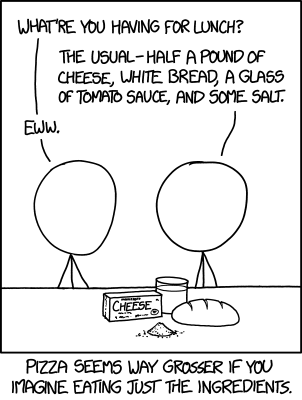
\includegraphics[width=0.4\hsize]{info/xkcd/lunch.png}
\end{center}

\pagebreak

\end{description}


\else
	Damit ihr nicht ganz verloren im gro\ss en Uni-Wirrwarr umher irrt und
  nicht immer das Gefühl haben müsst, etwas sehr Wichtiges geht
  voll an euch vorbei, findet ihr hier eine Übersicht über die wichtigsten Begriffe:

\begin{description}

\item [Übungen:] Zu den Mathe- und Informatikvorlesungen werden neben den Vorlesungen noch Übungsblätter angeboten, welche euch helfen, den gelernten Stoff zu verinnerlichen. Meist könnt ihr über die Übungsblätter, die ihr wöchentlich oder zweiwöchentlich abgeben könnt, einen Bonus für eure Klausurnote erarbeiten. In machen Vorlesungen kann aber auch eine Mindestpunktzahl in den Übungen Voraussetzung für die Klausur sein.

Da die dazu zu lösenden Aufgaben manchmal recht heftig und zeitaufwändig ausfallen, empfiehlt es sich:

\begin{itemize}

\item \textbf{sofort voll einzusteigen}, denn die Aufgaben werden von Mal
  zu Mal schwerer.

\item sich eine \textbf{Arbeitsgruppe} zu suchen, denn alleine ist man
  als "`Normalbegabter"' fast verloren. Meistens darf eine
  Arbeitsgruppe (2-3 Studis) sogar eine gemeinsame Lösung abgeben!

\item auch dann Übungen zu machen, wenn es keine Pflichtaufgaben sind --
  die Klausur kommt bestimmt.

\end {itemize}

\begin{center}
\includegraphics[width=0.5\hsize]{shared/xkcd/efficiency.png}
\end{center}


(Don't panic -- Die Matheübungszettel sind zu Anfang zwar der gro\ss e
  Schocker, die Prüfungen laufen aber in gemä\ss igterem Rahmen ab.)

\item [Vorlesungen:] In den Vorlesungen wird euch der nötige Stoff vermittelt. Es empfiehlt sich bei jeder Vorlesung sich Notizen zu machen und die Vorlesung nachzuarbeiten, da die Notizen oft chaotisch und unübersichtlich sind. Welche Vorlesungen angeboten werden findet ihr im Vorlesungsverzeichnis.	%TODO insert \link{}{}?

\item [Vorlesungsverzeichnis:] Eine Übersicht über alle Veranstaltungen der Universität findet ihr in ALMA\footnote{\link{https://alma.uni-tuebingen.de}{ALMA}}. Dort findet ihr auch später eine Übersicht über eure Noten und könnt euch Studienbescheinigungen runterladen. Außerdem finden hier die Anmeldungen zu den Klausuren statt.	%TODO insert \link{}{}?

\item [ECTS, Credits, LP:] ECTS-Punkte (European Credit Transfer System, auch \textit{Credits} oder \textit{Leistungspunkte, LP}) sind seit der europaweiten Standardisierung von Bachelor- und Masterstudium (Bologna-Prozess\footnote{\url{https://de.wikipedia.org/wiki/Bologna-Prozess}}) die Währung, in der Leistung gemessen wird. 1 ECTS-Punkt entspricht ca. 30 Stunden Arbeit. Gibt eine Vorlesung 3 ECTS-Punkte, so müsst ihr in dem Semester ca. 90 Stunden für diese Vorlesung investieren. Habt ihr in den 15 Semesterwochen je zwei Stunden Vorlesung (also $15\cdot 2=30$ Stunden) durch Präsenzzeit investiert, so solltet ihr noch ca. 60 Stunden im Semester selbstständig für die Vorlesung investieren, um auf die vorgesehenen 90 Stunden zu kommen (vorbereiten, nachbereiten, zusammenfassen, auf die Klausur lernen).\\	%TODO insert \link{}{}?
Die Noten der jeweiligen Veranstaltungen werden mit deren ECTS-Punkten gewichtet.
 
\item [Eduroam:] Eduroam ist ein weltweiter Verbund von Bildungseinrichtungen, welcher es ermöglicht, an allen teilnehmenden Bildungseinrichtungen mit demselben Login ins Internet zu gehen.
Eine Anleitung, wie man Eduroam richtig einrichtet findet ihr im Infrastruktur-Kapitel.

\item [ZDV:] Das Zentrum für Datenverabeitung (ZDV) ist das Rechenzentrum der Universität und betreut die zahlreichen Rechner und Server, welche auch von Studierenden genutzt werden können. Vom ZDV solltet ihr nach eurer Immatrikulation auch ein Schreiben mit eurem ZDV Benutzernamen und einem Passwort bekommen haben. Diese ermöglichen euch die Nutzung der Uni-Infrastruktur.

\item [CIP Pool:] CIP Pools sind von der Universität betriebene Räume in denen Rechner des ZDVs stehen, die man als Studierender mit seiner ZDV Kennung nutzen kann.

\item[BAföG:] Das Bundesausbildungsförderungsgesetz unterstützt Studierende und Auszubildende aus einkommensschwachen Elternhäusern. Ob und wie ihr BAföG bekommt könnt ihr hier nachschauen: \url{http://www.bafoeg-rechner.de/}	%TODO insert \link{}{}?

\item[Mensa:] Die Mensen sind der Ort in dem man sich zum (un-)regelmäßigen Mittagessen trifft. Jede Mensa hat einen Speiseplan, welchen man auf der Seite des Studierendenwerks einsehen kann\footnote{\url{http://www.my-stuwe.de/mensa/}}.	%TODO insert \link{}{}?

\vfill

\end{description}
\pagebreak



	\subsection{Was erwartet euch?}
	Jetzt wo ihr euren Zeitplan der nächsten Wochen kennst, möchten wir euch noch ein paar Infos zu den Veranstaltungen geben, die euch im ersten Semester erwarten, damit ihr nichts wichtiges verpasst.

\subsubsection*{Informatik 1}
Informatik 1 ist die Grundlagenvorlesung der Informatik, in der ihr lernt zu programmieren. Hierfür sind keine Vorkenntnisse nötig. In der zweimal die Woche stattfindenden Vorlesung stellt euch der Professor immer neue Konzepte vor, welche ihr dann in den Übungen zuhause und im Tutorium üben könnt und solltet. Man hat meist eine Woche Zeit, die Aufgaben zu bearbeiten und abzugeben. Ein Tutor korrigiert diese und bespricht sie in einer Kleingruppe von ca 20 Studierenden mit euch. Durch die Übungen ist es darüber hinaus möglich, einen Bonus auf die Klausurnote zu erarbeiten. Hat man die Aufgaben immer sorgfältig gemacht, fällt einem die Klausur meist auch leichter.\\
Die Tutorien werden für gewöhnlich am Ende der ersten Woche eingeteilt. Genauere Informationen dazu gibt es in der ersten Vorlesung.

\begin{center}
\includegraphics[width=0.5\hsize]{info/xkcd/efficiency.png}
\end{center}

\subsubsection*{Mathe 1}
In Mathe 1 werden euch die Grundlagen der Mathematik beigebracht. Auch hier gibt es Übungsblätter und ein Tutorium in dem diese besprochen werden. Auch hier ist kontinuierliche Mitarbeit sehr zu empfehlen, da die Inhalte direkt aufeinander aufbauen.

\subsubsection*{Einführung in die Kognitionswissenschaft}
Die Einführung in die Kognitionswissenschaft ist eine der beiden Vorlesungen im ersten Semester, in der nur die Kognis sitzen. In dieser Veranstaltung wird euch ein Überblick über die einzelnen Felder der Kognitionswissenschaft gegeben, der fürs weitere Studium sehr nützlich ist.

\subsubsection*{Neurobiologie und Sinnesphysiologie}
In der Veranstaltung Neurobiologie und Sinnesphysiologie werden euch der Aufbau des Gehirns und die einzelnen Verarbeitungsmechanismen näher gebracht. Neben der Vorlesung müsst ihr noch eins von zwei Seminaren wählen, welche sich lediglich in der Uhrzeit unterscheiden. In diesen müsst ihr einen kleinen Vortrag im Themenfeld der Vorlesung halten.

\subsubsection*{Mathematische Statistik I}
In den empirischen Wissenschaften ist das Beherrschen von statistischen Methoden sehr wichtig. In dieser Veranstaltung wird euch der Teil der Statistik näher gebracht, welcher sich mit der Darstellung von empirischen Daten befasst (deskriptive Statistik). 




	\subsection{Die zukünftigen Semester}
	Nachdem ihr nun hoffentlich einen guten Blick über euer erstes Semester bekommen habt, möchten wir euch noch einen kleinen Ausblick auf künftige Semester geben. Welche Veranstaltungen ihr belegen müsst, um euren Bachelorabschluss zu bekommen, regeln Prüfungsordnung und Modulhandbuch\footnote{\url{https://uni-tuebingen.de/fakultaeten/mathematisch-naturwissenschaftliche-fakultaet/fachbereiche/informatik/studium/studiengaenge/kognitionswissenschaft/posmhbsdownloadsinfos/}}. Für euch gilt die Prüfungsordnung von 2017, d.h. der allgemeine Teil von 2015 in Kombination mit der Änderungssatzung 2017 sind relevant. Einen groben Überblick bekommt man aber schon durch den auf der nächsten Seite dargestellten Studienverlaufsplan.\\
\\
Die meisten Veranstaltungen in unserem Studium sind fest vorgegeben. Erst in den späteren Semestern haben wir vier Wahlpflichtmodule: Philosophie, Linguistik, Informatik und Kognition. In diesen Modulen könnt ihr aus den im ALMA\footnote{\url{https://alma.uni-tuebingen.de}} unter dem jeweiligen Modul aufgeführten Veranstaltungen frei wählen. Die Module, die ohne Mehraufwand anrechenbar sind, sind im Reiter Mein Studium -> Studienplaner mit Modulplan.\\
Außerdem habt ihr noch Wahlmöglichkeiten in den Modulen Experimentelle Kognitionswissenschaft und dem Teamprojekt. In experimenteller Kognitionswissenschaft werdet ihr die in den ersten Semestern erworbenen Grundlagen der empirischen Forschung kombiniert mit eurem dazu gewonnenen Wissen zum ersten Mal anwenden und in Kleingruppen jeweils ein Experiment durchführen. Wem dies Spaß macht kann im Teamprojekt wieder empirisch arbeiten und zum Beispiel auch neuere Methoden wie das Elektroenzephalogramm (EEG) verwenden. Wer es lieber technischer mag, kann auch ein eher informatiknahes Projekt mit Schwerpunkt auf künstliche Intelligenz oder Neuronale Netze wählen.

Neben diesen fachbezogenen Wahlbereichen gibt es noch den Bereich Studium Professionale, in dem ihr überfachliche Qualifikationen erlernen sollt. Da das Studium der Kognitionswissenschaft bereits sehr überfachlich ist, können hier alle Veranstaltungen der Uni außer Sportveranstaltungen angerechnet werden.

\newcolumntype{C}[1]{>{\centering\arraybackslash}p{#1}}

\begin{tabular}{| C{0.14\textwidth} | C{0.14\textwidth} | C{0.14\textwidth} | C{0.14\textwidth} | C{0.14\textwidth} | C{0.14\textwidth} |} \hline
 1. Semester & 2. Semester & 3. Semester & 4. Semester & 5. Semester & 6. Semester\\ \hline \hline
 & & & & & \\
 & & & & \scriptsize{Computational} & \\
 & & & & \scriptsize{Neuroscience} & \\
 \scriptsize{Mathematik I} & \scriptsize{Mathematik II} & \scriptsize{Mathematik III} & \scriptsize{WPF Teamprojekt} &  \scriptsize{\textcolor{gray}{6 LP}} & \\
 \scriptsize{\textcolor{gray}{9 LP}} & \scriptsize{\textcolor{gray}{9 LP}} & \scriptsize{\textcolor{gray}{9 LP}} & \scriptsize{\textcolor{gray}{9 LP}} & &  \\
 & & & & & \scriptsize{Bachelorarbeit} \\ \cline{5-5}
 & & & & & \scriptsize{inkl. Vortrag} \\
 & & & & \scriptsize{Kognitions-} & \scriptsize{\textcolor{gray}{15 LP}} \\
 & & & & \scriptsize{informatik} & \\ \cline{1-4}
 
 & & & & \scriptsize{\textcolor{gray}{6 LP}} & \\
 & & & & & \\
 & & & \scriptsize{Philosophie} & & \\ \cline{5-5}
 \scriptsize{Informatik I} & \scriptsize{Informatik II} & \scriptsize{Algorithmen} & \scriptsize{\textcolor{gray}{6 LP}} & & \\
 \scriptsize{\textcolor{gray}{9 LP}} & \scriptsize{\textcolor{gray}{9 LP}} & \scriptsize{\textcolor{gray}{9 LP}} & & & \\
 & & & & & \\ \cline{4-4}\cline{6-6}
 & & & \cellcolor{lightgray} & & \\
 & & & \cellcolor{lightgray} & \scriptsize{Vertiefung} & \scriptsize{Studium} \\
 & & & \cellcolor{lightgray} & \scriptsize{Kognitions-} & \scriptsize{Professionale} \\ \cline{1-4}
 
 \scriptsize{Einf. in d.} & \scriptsize{Methoden d.} & & & \scriptsize{wissenschaft} & \scriptsize{(überfachl.} \\
 \scriptsize{KogWis.} & \scriptsize{empir. Forschung} & \scriptsize{Linguistik für} & \scriptsize{Language \&} & \scriptsize{\textcolor{gray}{12 LP}}  & \scriptsize{Kompetenzen,} \\
 \scriptsize{\textcolor{gray}{3 LP}} & \scriptsize{\textcolor{gray}{3 LP}} & \scriptsize{Kognitions-} & \scriptsize{Cognition} & & \scriptsize{übK)} \\ \cline{1-2} 
 
 \scriptsize{Mathemath.} & \scriptsize{Mathemath.} & \scriptsize{wissenschaftler} & \scriptsize{\textcolor{gray}{6 LP}} & & \scriptsize{\textcolor{gray}{9 LP}} \\
 \scriptsize{Statistik I} & \scriptsize{Statistik II} & \scriptsize{\textcolor{gray}{6 LP}} & & & \\
 \scriptsize{\textcolor{gray}{3 LP}} & \scriptsize{\textcolor{gray}{3 LP}} & & & & \\ \cline{1-6}
 
 & \scriptsize{Computergest.} & & \scriptsize{Kognitive} & \scriptsize{Forschungs-} & \scriptsize{Forschungs-} \\
 \scriptsize{Neurobiologie u.} & \scriptsize{Statistik} & \scriptsize{Experimentelle} & \scriptsize{Architekturen} & \scriptsize{seminar} &  \scriptsize{seminar} \\
 \scriptsize{Sinnesphysiol.} & \scriptsize{\textcolor{gray}{3 LP}} & \scriptsize{Kognitionswiss.} & \scriptsize{\textcolor{gray}{3 LP}} & \scriptsize{\textcolor{gray}{3 LP}} & \scriptsize{\textcolor{gray}{3 LP}} \\ \cline{2-2} \cline{4-6}
 
 \scriptsize{\textcolor{gray}{6 LP}} & \scriptsize{Allgemeine} &  \scriptsize{\textcolor{gray}{6 LP}} & \scriptsize{Psychologie} & \scriptsize{Psychologie} & \scriptsize{Forschungs-} \\
 & \scriptsize{Psychologie C} & & \scriptsize{\textcolor{gray}{3 LP}} & \scriptsize{\textcolor{gray}{3 LP}} & \scriptsize{Kolloquium} \\
 & \scriptsize{\textcolor{gray}{3 LP}} & & & & \scriptsize{\textcolor{gray}{3 LP}} \\
\hline
 \cellcolor{lightgray} & \cellcolor{lightgray} & \scriptsize{Allgemeine} & \cellcolor{lightgray} & \cellcolor{lightgray} & \cellcolor{lightgray} \\
 \cellcolor{lightgray} & \cellcolor{lightgray} & \scriptsize{Psychologie B} & \cellcolor{lightgray} & \cellcolor{lightgray} & \cellcolor{lightgray} \\
 \cellcolor{lightgray} & \cellcolor{lightgray} & \scriptsize{\textcolor{gray}{3 LP}} & \cellcolor{lightgray} & \cellcolor{lightgray} & \cellcolor{lightgray} \\ 
 \hline \hline
 30 LP & 30 LP & 33 LP & 27 LP & 30 LP & 30 LP \\
 \hline
\end{tabular} 



	\pagebreak

	\subsection{Die ersten Wochen}
	Auf den folgenden vier Seiten haben wir euch die wichtigsten Termine der kommenden vier Wochen nochmal zusammengefasst. Eine Einladung mit ausführlichen Beschreibungen der Erstsemesterveranstaltungen solltet ihr schon mit eurem Erstibrief\footnote{\url{http://www.fsi.uni-tuebingen.de/erstsemester/material/start}} bekommen haben.
\vfill



\definecolor{lightlightgray}{RGB}{235,235,235}

%\newpage
\textbf{Woche 1 - (02. Oktober - 06. Oktober)}\\
\\
\begin{tabular}{|l|p{0.15\textwidth}|p{0.15\textwidth}|p{0.15\textwidth}|p{0.15\textwidth}|p{0.15\textwidth}|} \hline
 Zeit & Montag & Dienstag & Mittwoch & Donnerstag & Freitag \\ 
 \hline \hline
 08 -- 09 & & & & & \\ \cline{1-1} 
\cline{2-6}
 09 -- 10 &\footnotesize{Mathe Vorkurs} & \footnotesize{Feiertag} &\footnotesize{Mathe Vorkurs} & \footnotesize{Mathe Vorkurs} & \footnotesize{Mathe Vorkurs} \\ \cline{1-1}
 10 -- 11 & & & & & \\ \cline{1-1}
 11 -- 12 & & & & & \\ \cline{1-1}
 12 -- 13 & & & & & \\ \cline{1-1} 
 13 -- 14 & & & & & \\ \cline{1-1}
 14 -- 15 & & & & & \\ \cline{1-1}
 15 -- 16 & & & & & \\ \cline{1-2}\cline{4-6}
 16 -- 17 & & & & & \\ \cline{1-1}
 17 -- 18 & & & & &  \cellcolor{lightlightgray} \footnotesize{Grillen}\\ \cline{1-1} \cline{6-6}	
 18 -- 19 & & & & & \cellcolor{lightlightgray} \\ \cline{1-1}
 19 -- 20 & & &\cellcolor{lightlightgray} \footnotesize{Spieleabend} & & \cellcolor{lightlightgray}   \\ \cline{1-1}
 20 -- 21 & & &\cellcolor{lightlightgray} & &\cellcolor{lightlightgray}  \\ \cline{1-1}
 21 -- 22 & & &\cellcolor{lightlightgray} & & \cellcolor{lightlightgray}\\ \hline
 \end{tabular}
\vfil

\textbf{Woche 2 - (9. - 13. Oktober)}\\
\\
\begin{tabular}{|l|p{0.15\textwidth}|p{0.15\textwidth}|p{0.15\textwidth}|p{0.15\textwidth}|p{0.15\textwidth}|} \hline
 Zeit & Montag & Dienstag & Mittwoch & Donnerstag & Freitag \\ \hline \hline
 08 -- 09 & & & & & \\ \cline{1-5}
 09 -- 10 & \footnotesize{Mathe Vorkurs} & \footnotesize{Mathe Vorkurs} & \footnotesize{Mathe Vorkurs} & \footnotesize{Mathe Vorkurs} &  \\ \cline{1-1}
 10 -- 11 & & & & &\cellcolor{lightlightgray} \scriptsize{Ersti-Frühstück} \\ \cline{1-1}
 11 -- 12 & & & & & \\ \cline{1-1}
 12 -- 13 & & & & & \\ \cline{1-1}
 13 -- 14 & & & & & \\ \cline{1-1}
 14 -- 15 & & & & & \\ \cline{1-1}
 15 -- 16 & & & & & \\ \cline {1-5}
 16 -- 17 & & & & & \\ \cline{1-1}
 17 -- 18 & & & & & \\ \cline{1-1}
 18 -- 19 & &\cellcolor{lightlightgray} \footnotesize{Kneipentour} & & & \\ \cline{1-1}
 19 -- 20 & &\cellcolor{lightlightgray}  & & & \\ \cline{1-1}
 20 -- 21 & &\cellcolor{lightlightgray}  & & &  \\ \cline{1-1}
 21 -- 22 & &\cellcolor{lightlightgray}  & & & \\ \hline
\end{tabular}
\\
\scriptsize{TBA = to be announced. Wird auf Fachschaftswebsite\footnote{\url{https://www.fsi.uni-tuebingen.de/erstsemester/veranstaltungen/start}}  bekanntgegeben.} \\
\scriptsize{Grau unterlegt = Veranstaltungen der Fachschaften Informatik und Kognitionswissenschaft }
\newpage


\textbf{Woche 3 - (16. - 20. Oktober)}\\
\\
\begin{tabular}{|l|p{0.15\textwidth}|p{0.15\textwidth}|p{0.15\textwidth}|p{0.15\textwidth}|p{0.15\textwidth}|} \hline
	Zeit & Montag & Dienstag & Mittwoch & Donnerstag & Freitag \\ 
	\hline \hline
 08 -- 09 & \footnotesize{Mathematik 1} & & \footnotesize{Mathematik 1} & & \\ \cline{1-1}
 09 -- 10 & & & & & \\ \cline{1-5}
 10 -- 11 & \footnotesize{Tierphysiologie: Neurobio und Sinnesphysio.} & \footnotesize{Einf. in die Kogwiss.} & & \footnotesize{Statistik I} & \\ \cline{1-1} 
 11 -- 12 &  &  & &  & \\ \hline
 12 -- 13 & \footnotesize{Computergest. Statistik 1 (Gruppe 1)}& & & & \\ \cline{1-1}
 13 -- 14 & & & & & \\ \hline
 14 -- 15 & \footnotesize{Computergest. Statistik 1 (Gruppe 2)} & \footnotesize{Informatik 1} & & \footnotesize{Informatik 1} & \\  \cline {1-1}
 15 -- 16 & &  & & & \\ \hline
 16 -- 17 & & & & & \\ \cline{1-1}
 17 -- 18 & & & & & \\ \cline{1-1} \cline{4-5}
 18 -- 19 & & & & \scriptsize{Ersti-Kneipentour} \cellcolor{lightlightgray}& \scriptsize{Stadtrallye} \cellcolor{lightlightgray}\\ \cline{1-1}
 19 -- 20 & & &\scriptsize{Spieleabend} \cellcolor{lightlightgray} & \cellcolor{lightlightgray} & \cellcolor{lightlightgray}\\ \cline{1-1}
 20 -- 21 & & &\cellcolor{lightlightgray} &  \cellcolor{lightlightgray}& \cellcolor{lightlightgray}\\ \cline{1-1}
 21 -- 22 & & &\cellcolor{lightlightgray} &  \cellcolor{lightlightgray}& \cellcolor{lightlightgray}\\ \hline
\end{tabular}

\scriptsize{B.Sc. = Bachelor ~|~ M.Sc. = Master ~|~ PI = Psychologisches Institut - Schleichstraße 4 ~|~ HSZ = Hörsaalzentrum (Morgenstelle)}
\\
\\
\scriptsize{Außerdem gibt es Veranstaltungen am Wochenende, wie wandern oder Capture The Flag. Schaut bei eei.fsi.uni-tuebingen.de vorbei!}
\vfil
\textbf{Woche 4 - (23. - 27. Oktober)}\\
\\
\begin{tabular}{|l|p{0.15\textwidth}|p{0.15\textwidth}|p{0.15\textwidth}|p{0.15\textwidth}|p{0.15\textwidth}|} \hline
	Zeit & Montag & Dienstag & Mittwoch & Donnerstag & Freitag \\ 
	\hline \hline
 08 -- 09 & \footnotesize{Mathematik 1} & & \footnotesize{Mathematik 1} & & \\ \cline{1-1}
 09 -- 10 & & & & & \\ \cline{1-5}
 10 -- 11 & \footnotesize{Tierphysiologie: Neurobio und Sinnesphysio.} & \footnotesize{Einf. in die Kogwiss.} & & \footnotesize{Statistik I} & \\ \cline{1-1} 
 11 -- 12 &  &  & &  & \\ \hline
 12 -- 13 & \footnotesize{Computergest. Statistik 1 (Gruppe 1)}& & & & \\ \cline{1-1}
 13 -- 14 & & & & & \\ \hline
 14 -- 15 & \footnotesize{Computergest. Statistik 1 (Gruppe 2)} & \footnotesize{Informatik 1} & & \footnotesize{Informatik 1} & \\  \cline {1-1}
 15 -- 16 & &  & & & \\ \hline
 16 -- 17 & &  & & & \\ \cline{1-1}
 17 -- 18 & & & \scriptsize{Grillen} \cellcolor{lightlightgray}& &\\ \cline{1-1} \cline{4-4}
 18 -- 19 & &\scriptsize{Ersti Filmeabend} \cellcolor{lightlightgray} & \cellcolor{lightlightgray}& & \\ \cline{1-1}
 19 -- 20 & & \cellcolor{lightlightgray} & \cellcolor{lightlightgray} & & \\ \cline{1-1}
 20 -- 21 & & \cellcolor{lightlightgray} & \cellcolor{lightlightgray} & & \\ \cline{1-1}
 21 -- 22 & & \cellcolor{lightlightgray} & \cellcolor{lightlightgray} & & \\ \hline
\end{tabular}


\footnotesize{Eventuell finden in dieser Woche schon Tutorien beziehungsweise das Seminar zu Neurobiologie und Sinnesphysiologie statt. Informationen dazu bekommt ihr in den jeweiligen Vorlesungen.}
\normalsize
\newpage

\fi

\pagebreak

\subsection{Checkliste}
\ifinfo
	% erstewoche/checkliste.tex

Die ersten Wochen an der Uni sind erfahrungsgemäß die schlimmsten: Wir haben euch hier die wichtigsten Punkte zusammengestellt, um die ihr euch in den ersten Tagen bzw. Wochen kümmern solltet. Man findet sich im großen Chaos Universität ziemlich schnell zurecht -- Don't panic!
  
  \begin{enumerate}[label=$\bigcirc$]
  	
  	\item \textbf{Zum Übungsbetrieb anmelden} \\
	  	Oft muss man, um zur Klausur einer Veranstaltung zugelassen zu werden, eine bestimmte Anzahl an Punkten in den Übungsblättern erreichen. Damit ihr die Übungen machen könnt, müsst ihr euch in der Veranstaltung dazu anmelden. Wie das geht, erfahrt ihr in den ersten Vorlesungen (oft sogar direkt in der ersten Vorlesung, also nicht verpassen!).
  	\item \textbf{Übungspartner suchen} \\
	  	Übungsblätter im Alleingang zu machen ist zwar möglich, aber schwierig. Sucht euch daher am besten gleich am Anfang pro Veranstaltung mit Übungsbetrieb einen Übungspartner, mit dem ihr die Blätter abgeben könnt.
  	\item \textbf{WLAN-Zugang mit eduroam einrichten}\\
	  	Mit euren ZDV-Login-Daten (i.d.R. \texttt{zxabc12@uni-tuebingen.de} und dem ZDV-Passwort) könnt ihr uni-weit kostenlos per WLAN ins Internet. \textbf{Wichtig:} Bindet ein Zertifikat ein! Eine ausführliche Anleitung hierzu findet ihr im Kapitel Infrastruktur.
  	\item \textbf{Erstwohnsitz in Tübingen anmelden} \\
	  	Sofern ihr mit dem Studienbeginn neu nach Tübingen gezogen seid, solltet ihr euch innerhalb von zwei Wochen bei der Stadtverwaltung anmelden. Hierfür benötigt ihr eine Kopie des Mietvertrages und die Wohnungsgeberbescheinigung. Es ist ratsam, seinen Erstwohnsitz in Tübingen anzumelden und z.B. das elterliche Wohnhaus als Zweitwohnsitz anzugeben, da Tübingen eine Zweitwohnsitzsteuer erhebt.
	\item \textbf{Postadresse im CAMPUS aktualisieren}\\
		Die ZV der Uni schickt euch jedes Semester nachdem ihr euch erfolgreich rückgemeldet habt euer neues Datenkontrollblatt zu, in dem ihr u.A. die Bescheinigung für das Semesterticket findet. Damit dieser Brief nicht immer an die falsche Adresse geht, solltet ihr im CAMPUS-System eure Adresse aktualisieren.
	\item \textbf{Rundfunkbeitrag} \\
		Diesen Brief bekommt ihr normalerweise, sobald ihr euch nach Tübingen umgemeldet habt. Die Rundfunkgebühren müssen nur von einer Person pro Haushalt bezahlt werden, fragt also eure Mitbewohner oder Vermieter, ob schon bezahlt wird! Wenn ihr BaföG bezieht, könnt ihr euch u.U. vom Rundfunkbeitrag befreien lassen. Mehr Infos hierzu auch unter \url{https://www.rundfunkbeitrag.de/}.
  \end{enumerate}

\begin{center}
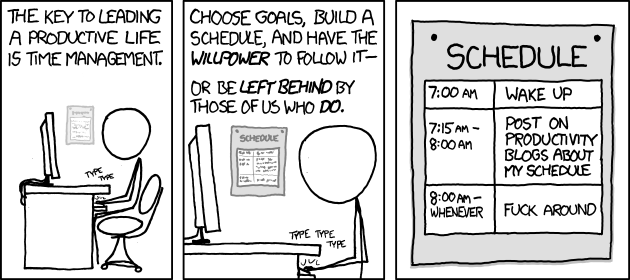
\includegraphics[width=0.5\hsize]{info/xkcd/time_management.png}
\end{center}


\else
	Da in der ersten Woche immer viel los ist, haben wir hier eine kleine Checkliste mit Dingen geschrieben, die ihr auf gar keinen Fall vergessen haben solltet:
\begin{enumerate}[label=$\bigcirc$]
	\item  \textbf{Erstwohnsitz umgemeldet} \\
	Hierzu müsst ihr zum Bürgeramt und euren Mietvertrag und eine Wohnungsgeberbescheinigung (bekommt ihr von eurem Vermieter) mitbringen. Die Ummeldung dauert für gewöhnlich nur wenige Minuten, normalerweise hat man jedoch etwas Wartezeit.
	
	\item \textbf{Rundfunkbeitrag angemeldet}\\
	Diesen Brief bekommt ihr normalerweise, sobald ihr euch nach Tübingen umgemeldet habt. Den Rundfunkbeitrag muss aber nur eine Person pro Haushalt bezahlen. Fragt deshalb am besten eure Mitbewohner, ob diesen schon jemand bezahlt.	
	
	\item  \textbf{Wohnadresse in Campus aktualisiert}\\
	Da die Uni euch hin und wieder wichtige Post schickt, benötigt sie eure aktuelle Adresse. Diese könnt ihr über das CAMPUS-System ändern.
	
	\item \textbf{WLAN-Zugang mit Eduroam eingerichtet}\\
	Mit deinen ZDV-Login-Daten könnt ihr europaweit an allen teilnehmenden Universitäten ins Internet.
	
	\item  \textbf{Neurobiologie und Sinnesphysiologie Seminar gewählt}\\
	Hierzu geht für gewöhnlich in der ersten Vorlesung eine Liste rum, in die man sich ganz altmodisch per Stift eintragen muss. Sollte man in der ersten Vorlesung nicht anwesend sein können, kann man Herrn Mallot auch eine Mail schicken.
	
	\item  \textbf{Zum Übungsbetrieb angemeldet}\\
	Bei Informatik 1 und Mathe 1 muss man, um zur Klausur zugelassen zu werden, eine bestimmte Anzahl an Punkten in den Übungsblättern erreichen. Damit ihr die Übungen
machen könnt, müsst ihr euch in der Veranstaltung dazu anmelden. Wie das geht,
erfahrt ihr in den ersten Vorlesungen (oft sogar direkt in der ersten Vorlesung, also
nicht verpassen!).

	\item \textbf{Auf Versuchspersonen-Listen anmelden}\\
	In den ersten drei Semestern müssen alle Kognis 30 Stunden als Versuchsperson für psychologische Experimente zur Verfügung stehen (Mehr dazu im Abschnitt \textit{Die Versuchspersonenstunden}). Zu den Experimenten anmelden könnt ihr euch unter der Versuche-Mailingliste (Siehe Abschnitt \textit{Mailinglisten}) oder in der Facebook-Gruppe \textit{Versuchspersonenbörse Tübingen}.
	
	
\end{enumerate}
\fi

%******************************************************

%\pagebreak
\ifinfo
        \vspace{-1em} % TODO: Remove
\fi
\section{Die Vorlesungszeit}
\ifinfo
	\subsection{Der Stundenplan}
	Einen Beispielstundenplan für euer erstes Semester habt ihr bereits mit unserem
Anfibrief erhalten. Solltet ihr den Brief nicht mehr haben oder ihn nicht
bekommen haben, könnt ihr ihn euch auf unserer
Website\footnote{\link{https://teri.fsi.uni-tuebingen.de/anfibrief/}{Anfibrief
der FSI}} nochmal runterladen.\\ 
Im hinteren Teil des Hefts findet ihr einen Plan zum selbst ausfüllen, in dem
ihr euren finalen Stundenplan inklusive
Tutorien, Treffen mit Übungspartnern etc. eintragen könnt.

\coronabox{Da in diesem Semester viele der sonst langjährig etablierten
Übungsbetriebe umorganisiert werden müssen, ist es sehr wahrscheinlich, dass es
kurzfristig zu Änderungen kommt, und auch die DozentInnen noch nicht genau
sagen können, wie das Semester ablaufen wird. Informiert euch am besten
regelmäßig auf den entsprechenden Webseiten (z.B. Alma, Webseiten der
DozentInnen) zum aktuellen Stand der Dinge.}

	In höheren Semestern wird von euch erwartet werden, euren Stundenplan entsprechend eurer Prüfungsordnung und eures Modulhandbuches selbst zusammenzusuchen.
Dies bedeutet oft mehrere Stunden mit geöffnetem CAMPUS, PDF-Dateien sowie Stift und Zettel. Um euch bereits jetzt einen Überblick zu bieten,
was euch nach dem ersten Semester erwartet, haben wir für euch hier die so genannten Studienverlaufspläne zusammengefasst. Diese Pläne sind eine \textbf{Empfehlung}, wie ihr euer Studium gestalten könnt. Ihr müsst euch keinesfalls streng an diese Reihenfolge halten! \medskip
\\
\textbf{Für alle} Informatiker gilt: Ihr müsst eine je nach eurem Studiengang eine unterschiedliche Anzahl an Punkten aus dem \textbf{Studium Professionale} leisten. Oft ist in Prüfungsordnungen und Modulhandbüchern auch von \emph{überfachliche[n] berufsfeldorientierte[n] Kompetenzen} oder \emph{Schlüsselqualifikationen} die Rede. Offiziell geht es hier um das Programm der Uni, in der Praxis kann jedoch alles gewählt werden, das eine Prüfungleistung beinhaltet, für welche man einen benoteten Schein bekommt.\footnote{Abgesehen von Sportkursen.} Oft lohnt es sich auch, sich aus der eigenen comfort zone herauszubewegen und z.B. ein Seminar in den Geisteswissenschaften zu besuchen. \\Außerdem beinhalten alle Studiengänge das \textbf{Teamprojekt}, dies ist ein von einem Lehrstuhl angebotenes Programmier- bzw. Forschungsprojekt, welches ihr in kleineren Gruppen absolvieren müsst. Hier sammelt ihr erste Erfahrungen im teambasierten Arbeiten, setzt euch mit Versionierungssystemen etc. auseinander und erhaltet einen Einblick in die agile Softwareentwicklung.
\vfill \pagebreak 
\subsection*{Informatik}
	%\begin{table}[htbp]
%	\resizebox{\textwidth}{!}{
%		\begin{tabular}{|cccccc|}
%			\hline
%			1. Semester                            & 2. Semester                           & 3. Semester                           & 4. Semester                        & 5. Semester                           & 6. Semester    \\ \hline
%			\multicolumn{1}{|c|}{}                 & \multicolumn{1}{c|}{}                 & \multicolumn{1}{c|}{}                 & \multicolumn{1}{c|}{Mathematik IV} & \multicolumn{1}{c|}{WPF Praktische}   &                \\
%			\multicolumn{1}{|c|}{Mathematik I}     & \multicolumn{1}{c|}{Mathematik II}    & \multicolumn{1}{c|}{Mathematik III}   & \multicolumn{1}{c|}{}              & \multicolumn{1}{c|}{Informatik}       &                \\ \cline{4-5}
%			\multicolumn{1}{|c|}{}                 & \multicolumn{1}{c|}{}                 & \multicolumn{1}{c|}{}                 & \multicolumn{1}{c|}{Theoretische}  & \multicolumn{1}{c|}{WPF Theoretische} & Wahlpflicht    \\ \cline{1-3}
%			\multicolumn{1}{|c|}{Praktische}       & \multicolumn{1}{c|}{Praktische}       & \multicolumn{1}{c|}{}                 & \multicolumn{1}{c|}{Informatik}    & \multicolumn{1}{c|}{Informatik}       & Informatik B   \\ \cline{5-5}
%			\multicolumn{1}{|c|}{Informatik I}     & \multicolumn{1}{c|}{Informatik II}    & \multicolumn{1}{c|}{Algorithmen}      & \multicolumn{1}{c|}{}              & \multicolumn{1}{c|}{WPF Technische}   &                \\ \cline{4-4} \cline{6-6} 
%			\multicolumn{1}{|c|}{}                 & \multicolumn{1}{c|}{}                 & \multicolumn{1}{c|}{}                 & \multicolumn{1}{c|}{}              & \multicolumn{1}{c|}{Informatik}       &                \\ \cline{1-3} \cline{5-5}
%			\multicolumn{1}{|c|}{Technische}       & \multicolumn{1}{c|}{Technische}       & \multicolumn{1}{c|}{Praktikum}        & \multicolumn{1}{c|}{Teamprojekt}   & \multicolumn{1}{c|}{Wahlpflicht}      &                \\
%			\multicolumn{1}{|c|}{Informatik I}     & \multicolumn{1}{c|}{Informatik II}    & \multicolumn{1}{c|}{Tech. Informatik} & \multicolumn{1}{c|}{}              & \multicolumn{1}{c|}{Informatik A}     & Bachelorarbeit \\ \cline{1-5}
%			\multicolumn{1}{|c|}{Studium}      	   & \multicolumn{1}{c|}{Logik}            & \multicolumn{1}{c|}{Schwerpunkt}      & \multicolumn{1}{c|}{Schwerpunkt}   & \multicolumn{1}{c|}{Schwerpunkt}      &                \\ \cline{2-2} \cline{5-5}
%			\multicolumn{1}{|c|}{Professionale}    & \multicolumn{1}{c|}{Proseminar}       & \multicolumn{1}{c|}{}                 & \multicolumn{1}{c|}{}              & \multicolumn{1}{c|}{}					&                \\ \hline
%			30 LP                                  & 30 LP                                 & 30 LP                                 & 30 LP                              & 30 LP                                 & 30 LP          \\ \hline
%		\end{tabular}}
%\end{table}

% PO 2021
\begin{table}[htbp]
\resizebox{\textwidth}{!}{
\begin{tabular}{|cccccc|}
\hline
1.Semester                         & 2. Semester                         & 3. Semester                         & 4. Semester                              & 5. Semester                      & 6. Semester    \\ \hline
\multicolumn{1}{|c|}{Praktische}   & \multicolumn{1}{c|}{Praktische}     & \multicolumn{1}{c|}{Theoretische}   & \multicolumn{1}{c|}{Theoretische}        & \multicolumn{1}{c|}{Proseminar}  & übK            \\ \cline{5-5}
\multicolumn{1}{|c|}{Informatik I} & \multicolumn{1}{c|}{Informatik II}  & \multicolumn{1}{c|}{Informatik I}   & \multicolumn{1}{c|}{Informatik II}       & \multicolumn{1}{c|}{Wahlpflicht} &                \\ \cline{6-6}
\multicolumn{1}{|c|}{}             & \multicolumn{1}{c|}{}               & \multicolumn{1}{c|}{}               & \multicolumn{1}{c|}{}                    & \multicolumn{1}{c|}{Prakt. Inf.} & Wahlpflicht    \\ \cline{1-5}
\multicolumn{1}{|c|}{}             & \multicolumn{1}{c|}{}               & \multicolumn{1}{c|}{}               & \multicolumn{1}{c|}{Mathematik IV}       & \multicolumn{1}{c|}{Wahlpflicht} & Informatik     \\ \cline{6-6}
\multicolumn{1}{|c|}{Mathematik I} & \multicolumn{1}{c|}{Mathematik II}  & \multicolumn{1}{c|}{Mathematik III} & \multicolumn{1}{c|}{}                    & \multicolumn{1}{c|}{Theo. Inf.}  &                \\ \cline{4-5}
\multicolumn{1}{|c|}{}             & \multicolumn{1}{c|}{}               & \multicolumn{1}{c|}{}               & \multicolumn{1}{c|}{Praktische}          & \multicolumn{1}{c|}{übK}         &                \\ \cline{1-3}
\multicolumn{1}{|c|}{Technische}   & \multicolumn{1}{c|}{Technische}     & \multicolumn{1}{c|}{Praktische}     & \multicolumn{1}{c|}{Informatik IV:}      & \multicolumn{1}{c|}{}            & Bachelorarbeit \\ \cline{5-5}
\multicolumn{1}{|c|}{Informatik I} & \multicolumn{1}{c|}{Informatik II}  & \multicolumn{1}{c|}{Informatik III} & \multicolumn{1}{c|}{Teamprojekt}         & \multicolumn{1}{c|}{Wahlpflicht} &                \\ \cline{1-1} \cline{3-4}
\multicolumn{1}{|c|}{übK}          & \multicolumn{1}{c|}{}               & \multicolumn{1}{c|}{Wahlpflicht}    & \multicolumn{1}{c|}{Grundlagen d.}       & \multicolumn{1}{c|}{Informatik}  &                \\ \cline{2-2} \cline{6-6}
\multicolumn{1}{|c|}{}             & \multicolumn{1}{c|}{Technische}     & \multicolumn{1}{c|}{Techn. Inf.}    & \multicolumn{1}{c|}{Machinellen Lernens} & \multicolumn{1}{c|}{}            &                \\ \cline{1-1} \cline{3-5}
\multicolumn{1}{|c|}{}             & \multicolumn{1}{c|}{Informatik III} & \multicolumn{1}{c|}{}               & \multicolumn{1}{c|}{}                    & \multicolumn{1}{c|}{}            &                \\ \hline
30 ECTS                            & 33 ECTS                             & 30 ECTS                             & 30 ECTS                                  & 30 ECTS                          & 27 ECTS        \\ \hline
\end{tabular}}
\end{table}

Abgesehen vom Standardprogramm (Informatik I-III, Mathematik I-III) ist es im Studienplan der Informatik bereits im ersten Semester vorgesehen, Punkte aus dem Bereich des Studium Professionale zu sammeln.  Das Schwerpunktfach (auch Nebenfach genannt) ist ab dem dritten Semester vorgesehen, ihr solltet euch also im zweiten Semester darum kümmern, was ihr als Schwerpunkt wählen wollt und welche Leistungen ihr hierfür erbringen müsst.
\subsection*{Informatik Lehramt}
	% Please add the following required packages to your document preamble:
% \usepackage[normalem]{ulem}
% \useunder{\uline}{\ul}{}
% \begin{table}[htbp]
%	\resizebox{\textwidth}{!}{
%		\begin{tabular}{|ccccccc|}
%			\hline
%			Fachsemester             & LP                      & \multicolumn{2}{c}{Pflicht}                                                                                                                                                                                         & Wahlpflicht                                                                              & Fachdidaktik                                                                          & Bachelorarbeit                                                  \\ \hline
%			\multicolumn{1}{|c|}{1.} & \multicolumn{1}{c|}{15} & \multicolumn{1}{c|}{\begin{tabular}[c]{@{}c@{}}Informatik I \\ (9 LP)\end{tabular}}              & \multicolumn{1}{c|}{\begin{tabular}[c]{@{}c@{}}Einführung in die\\ Technische\\ Informatik\\ (6 LP)\end{tabular}} & \multicolumn{1}{c|}{}                                                                    & \multicolumn{1}{c|}{}                                                                 &                                                                 \\ \cline{1-4} \cline{6-6}
%			\multicolumn{1}{|c|}{2.} & \multicolumn{1}{c|}{12} & \multicolumn{2}{c|}{\begin{tabular}[c]{@{}c@{}}Informatik II\\ (9 LP)\end{tabular}}                                                                                                                                 & \multicolumn{1}{c|}{}                                                                    & \multicolumn{1}{c|}{\begin{tabular}[c]{@{}c@{}}Fachdidaktik I\\ (3 LP)\end{tabular}}  &                                                                 \\ \cline{1-4} \cline{6-6}
%			\multicolumn{1}{|c|}{3.} & \multicolumn{1}{c|}{15} & \multicolumn{2}{c|}{\begin{tabular}[c]{@{}c@{}}Mathematik I /\\ Ausgleichsmodul Mathematik\\ (9 LP)\end{tabular}}                                                                                                   & \multicolumn{1}{c|}{}                                                                    & \multicolumn{1}{c|}{\begin{tabular}[c]{@{}c@{}}Fachdidaktik II\\ (6 LP)\end{tabular}} &                                                                 \\ \cline{1-4} \cline{6-6}
%			\multicolumn{1}{|c|}{4.} & \multicolumn{1}{c|}{15} & \multicolumn{1}{c|}{\begin{tabular}[c]{@{}c@{}}Theoretische \\ Informatik\\ (9 LP)\end{tabular}} & \multicolumn{1}{c|}{\begin{tabular}[c]{@{}c@{}}Informatik\\ der Systeme\\ (6 LP)\end{tabular}}                    & \multicolumn{1}{c|}{}                                                                    & \multicolumn{1}{c|}{}                                                                 &                                                                 \\ \cline{1-5}
%			\multicolumn{1}{|c|}{5.} & \multicolumn{1}{c|}{12} & \multicolumn{2}{c|}{\begin{tabular}[c]{@{}c@{}}Algorithmen\\ (9 LP)\end{tabular}}                                                                                                                                   & \multicolumn{1}{c|}{\begin{tabular}[c]{@{}c@{}}Wahlpflichtmodul I\\ (3 LP)\end{tabular}} & \multicolumn{1}{c|}{}                                                                 &                                                                 \\ \cline{1-5} \cline{7-7} 
%			\multicolumn{1}{|c|}{6.} & \multicolumn{1}{c|}{12} & \multicolumn{2}{c|}{\begin{tabular}[c]{@{}c@{}}Teamprojekt\\ (9 LP)\end{tabular}}                                                                                                                                   & \multicolumn{1}{c|}{Wahlpflichtmodul}                                                    & \multicolumn{1}{c|}{}                                                                 & \begin{tabular}[c]{@{}c@{}}Bachelorarbeit\\ (6 LP)\end{tabular} \\ \hline
%		\end{tabular}}
%\end{table}

% Please add the following required packages to your document preamble:
% \usepackage[normalem]{ulem}
% \useunder{\uline}{\ul}{}
\begin{table}[htbp]
\resizebox{\textwidth}{!}{
\begin{tabular}{|c|c|c|c|c|c|c|}
\hline
FS & ECTS & \multicolumn{2}{c|}{Pflicht}                    & Wahlpflicht   & Fachdidaktik    & Bachelorarbeit \\ \hline
1  & 15   & Praktische              & Technische            &               &                 &                \\
   &      & Informatik I (9 LP)     & Informatik I (6 LP)   &               &                 &                \\ \hline
2  & 12   & \multicolumn{2}{c|}{Praktische Informatik II}   &               & Fachdidaktik I  &                \\
   &      & \multicolumn{2}{c|}{(9 LP)}                     &               & (3 LP)          &                \\ \hline
3  & 15   & Mathematik I /          & Praktische            &               &                 &                \\
   &      & Ausgleichsmodul (9 LP)  & Informatik III (6 LP) &               &                 &                \\ \hline
4  & 15   & \multicolumn{2}{c|}{Theoretische Informatik II} &               & Fachdidaktik II &                \\
   &      & \multicolumn{2}{c|}{(9 LP)}                     &               & (6 LP)          &                \\ \hline
5  & 12   & \multicolumn{2}{c|}{Theoretische Informatik I}  & Wahlpflicht I &                 &                \\
   &      & \multicolumn{2}{c|}{(9 LP)}                     & (3 LP)        &                 &                \\ \hline
6  & 12+6 & \multicolumn{2}{c|}{Technische Informatik II}   & Wahlpflicht I &                 & Bachelorarbeit \\
   &      & \multicolumn{2}{c|}{(9 LP)}                     & (3 LP)        &                 & (6 LP)         \\ \hline
\end{tabular}}
\end{table}

\pagebreak 
Der Stundenplan in Informatik für Lehramt kann recht flexibel belegt werden, da die Module unabhängig voneinander sind. Wer im Zweitfach Mathematik gewählt hat, darf kein Mathe 1 hören, muss aber dafür ein Ausgleichsmodul hören. Als Ausgleichsmodul kann man jedes Wahlpflichtmodul mit gleicher Anzahl an ETCS-Punkten wählen, welches in Campus angeboten wird. Für welche mit einer anderen Kombination als Mathe, ist das Ausgleichsmodul nicht relevant. Die Fachdidaktik-Veranstaltungen finden meist nicht zu den vorgesehen Zeiten im Studienplan statt, da sie teilnehmerabhängig sind. Stattdessen wird mit einer Umfragemail ein Termin gesucht. Die Antwort des Dozenten kann auch mal ein paar Monate auf sich warten lassen.

\subsection*{Bioinformatik}
	\begin{table}[htbp]
	\resizebox{\textwidth}{!}{		
		\begin{tabular}{cccccc}
			\hline
			\multicolumn{1}{|c}{1. Semester}    & 2. Semester                               & 3. Semester                           & 4. Semester                         & 5. Semester                            & \multicolumn{1}{c|}{6. Semester}          \\ \hline
			\multicolumn{1}{|c|}{}              & \multicolumn{1}{c|}{}                     & \multicolumn{1}{c|}{}                 & \multicolumn{1}{c|}{Theoretische}   & \multicolumn{1}{c|}{WPF Praktische}    & \multicolumn{1}{c|}{}                     \\
			\multicolumn{1}{|c|}{Informatik I}  & \multicolumn{1}{c|}{Informatik II}        & \multicolumn{1}{c|}{Algorithmen}      & \multicolumn{1}{c|}{Informatik}     & \multicolumn{1}{c|}{Informatik}        & \multicolumn{1}{c|}{}                     \\ \cline{5-5}
			\multicolumn{1}{|c|}{}              & \multicolumn{1}{c|}{}                     & \multicolumn{1}{c|}{}                 & \multicolumn{1}{c|}{}               & \multicolumn{1}{c|}{Chemie II}         & \multicolumn{1}{c|}{Bachelorarbeit}       \\ \cline{1-4}
			\multicolumn{1}{|c|}{}              & \multicolumn{1}{c|}{}                     & \multicolumn{1}{c|}{}                 & \multicolumn{1}{c|}{Stochastik}     & \multicolumn{1}{c|}{}                  & \multicolumn{1}{c|}{}                     \\ \cline{5-5}
			\multicolumn{1}{|c|}{Mathmematik I} & \multicolumn{1}{c|}{Mathematik II}        & \multicolumn{1}{c|}{Mathmematik III}  & \multicolumn{1}{c|}{}               & \multicolumn{1}{c|}{WPF Lebenswissen-} & \multicolumn{1}{c|}{}                     \\ \cline{4-4} \cline{6-6} 
			\multicolumn{1}{|c|}{}              & \multicolumn{1}{c|}{}                     & \multicolumn{1}{c|}{}                 & \multicolumn{1}{c|}{}               & \multicolumn{1}{c|}{schaften}          & \multicolumn{1}{c|}{Wahlpflicht}          \\ \cline{1-3} \cline{5-5}
			\multicolumn{1}{|c|}{Biomoleküle}  & \multicolumn{1}{c|}{Chemie I}             & \multicolumn{1}{c|}{Molekulare}       & \multicolumn{1}{c|}{Teamprojekt}    & \multicolumn{1}{c|}{Proseminar}        & \multicolumn{1}{c|}{Bioinformatik}        \\ \cline{5-6} 
			\multicolumn{1}{|c|}{und Zelle}     & \multicolumn{1}{c|}{(Teil B)}             & \multicolumn{1}{c|}{Biologie}         & \multicolumn{1}{c|}{}               & \multicolumn{1}{c|}{Studium}           & \multicolumn{1}{c|}{WPF Bioinfo / Info}   \\ \cline{1-4}
			\multicolumn{1}{|c|}{Chemie I}      & \multicolumn{1}{c|}{Einführung BioInfo.} & \multicolumn{1}{c|}{Neurobiologie}    & \multicolumn{1}{c|}{Grundlagen der} & \multicolumn{1}{c|}{Professionale}     & \multicolumn{1}{c|}{Lebenswissenschaften} \\ \cline{2-2} \cline{6-6} 
			\multicolumn{1}{|c|}{(Teil A)}      & \multicolumn{1}{c|}{}                     & \multicolumn{1}{c|}{}                 & \multicolumn{1}{c|}{Bioinformatik}  & \multicolumn{1}{c|}{}                  &                                           \\ \cline{1-1} \cline{3-3} \cline{5-5}
			                                    & \multicolumn{1}{c|}{}                     & \multicolumn{1}{c|}{Prakt. Neurobio.} & \multicolumn{1}{c|}{}               &                                        &                                           \\ \cline{3-4}
		\end{tabular}}
\end{table}
Das Bioinformatik-Studium beinhaltet in den ersten Semestern neben dem Standardprogramm der Informatik eine gute Portion Chemie und Zellbiologie. Später kommen dann Molekularbiologie (zusammen mit dem Studiengang molekulare Medizin) sowie noch mehr Chemie hinzu.
\pagebreak 
\subsection*{Medieninformatik}
	% \begin{table}[htbp]
% 	\resizebox{\textwidth}{!}{
% 		\begin{tabular}{cccccc}
% 			\hline
% 			\multicolumn{1}{|c}{1. Semester}     & 2. Semester                        & 3. Semester                            & 4. Semester                           & 5. Semester                            & \multicolumn{1}{c|}{6. Semester}      \\ \hline
% 			\multicolumn{1}{|c|}{}               & \multicolumn{1}{c|}{}              & \multicolumn{1}{c|}{}                  & \multicolumn{1}{c|}{Theoretische}     & \multicolumn{1}{c|}{Graphische}        & \multicolumn{1}{c|}{}                 \\
% 			\multicolumn{1}{|c|}{Informatik I}   & \multicolumn{1}{c|}{Informatik II} & \multicolumn{1}{c|}{Algorithmen}       & \multicolumn{1}{c|}{Informatik}       & \multicolumn{1}{c|}{Datenverarbeitung} & \multicolumn{1}{c|}{}                 \\
% 			\multicolumn{1}{|c|}{}               & \multicolumn{1}{c|}{}              & \multicolumn{1}{c|}{}                  & \multicolumn{1}{c|}{}                 & \multicolumn{1}{c|}{}                  & \multicolumn{1}{c|}{Bachelorarbeit}   \\ \cline{1-5}
% 			\multicolumn{1}{|c|}{}               & \multicolumn{1}{c|}{Informatik}    & \multicolumn{1}{c|}{}                  & \multicolumn{1}{c|}{WP Informatik /}  & \multicolumn{1}{c|}{Wahlpflicht}       & \multicolumn{1}{c|}{}                 \\
% 			\multicolumn{1}{|c|}{Mathmematik I}  & \multicolumn{1}{c|}{der Systeme}   & \multicolumn{1}{c|}{Mathmematik III}   & \multicolumn{1}{c|}{Medieninformatik} & \multicolumn{1}{c|}{Informatik /}      & \multicolumn{1}{c|}{}                 \\ \cline{2-2} \cline{4-4} \cline{6-6} 
% 			\multicolumn{1}{|c|}{}               & \multicolumn{1}{c|}{}              & \multicolumn{1}{c|}{}                  & \multicolumn{1}{c|}{WP Medienwiss.}   & \multicolumn{1}{c|}{Medieninformatik}  & \multicolumn{1}{c|}{Wahlpflicht}      \\ \cline{1-1} \cline{3-4}
% 			\multicolumn{1}{|c|}{User Interface} & \multicolumn{1}{c|}{Mathematik II} & \multicolumn{1}{c|}{Grundlagen der}    & \multicolumn{1}{c|}{}                 & \multicolumn{1}{c|}{}                  & \multicolumn{1}{c|}{Informatik /}     \\ \cline{5-5}
% 			\multicolumn{1}{|c|}{Design}         & \multicolumn{1}{c|}{}              & \multicolumn{1}{c|}{Multimediatechnik} & \multicolumn{1}{c|}{Teamprojekt}      & \multicolumn{1}{c|}{WP}                & \multicolumn{1}{c|}{Medieninformatik} \\ \cline{1-3} \cline{6-6} 
% 			\multicolumn{1}{|c|}{Einführung}    & \multicolumn{1}{c|}{Internet-}     & \multicolumn{1}{c|}{Bildverarbeitung}  & \multicolumn{1}{c|}{}                 & \multicolumn{1}{c|}{Medienwiss.}       & \multicolumn{1}{c|}{Studium}          \\ \cline{4-5}
% 			\multicolumn{1}{|c|}{Medienwiss.}    & \multicolumn{1}{c|}{technologien}  & \multicolumn{1}{c|}{}                  & \multicolumn{1}{c|}{Proseminar}       & \multicolumn{1}{c|}{Stud. Profess.}    & \multicolumn{1}{c|}{Professionale}    \\ \hline
% 			                                     &                                    &                                        &                                       &                                        &                                       
% 		\end{tabular}}
% \end{table}

% PO 2021
\begin{table}[htbp]
\resizebox{\textwidth}{!}{
\begin{tabular}{|cccccc|}
\hline
1.Semester                         & 2. Semester                        & 3. Semester                            & 4. Semester                           & 5. Semester                            & 6. Semester     \\ \hline
\multicolumn{1}{|c|}{Praktische}   & \multicolumn{1}{c|}{Praktische}    & \multicolumn{1}{c|}{Theoretische}      & \multicolumn{1}{c|}{Theoretische}     & \multicolumn{1}{c|}{Bildverarbeitung}  & Wahlpflicht     \\
\multicolumn{1}{|c|}{Informatik I} & \multicolumn{1}{c|}{Informatik II} & \multicolumn{1}{c|}{Informatik I}      & \multicolumn{1}{c|}{Informatik II}    & \multicolumn{1}{c|}{}                  & Medieninfo      \\ \cline{5-6} 
\multicolumn{1}{|c|}{}             & \multicolumn{1}{c|}{}              & \multicolumn{1}{c|}{}                  & \multicolumn{1}{c|}{}                 & \multicolumn{1}{c|}{Graphische}        & übK             \\ \cline{1-4}
\multicolumn{1}{|c|}{}             & \multicolumn{1}{c|}{}              & \multicolumn{1}{c|}{}                  & \multicolumn{1}{c|}{Praktische}       & \multicolumn{1}{c|}{Datenverarbeitung} &                 \\ \cline{6-6} 
\multicolumn{1}{|c|}{Mathematik I} & \multicolumn{1}{c|}{Mathematik II} & \multicolumn{1}{c|}{Mathematik III}    & \multicolumn{1}{c|}{Informatik IV:}   & \multicolumn{1}{c|}{}                  &                 \\ \cline{5-5}
\multicolumn{1}{|c|}{}             & \multicolumn{1}{c|}{}              & \multicolumn{1}{c|}{}                  & \multicolumn{1}{c|}{Teamprojekt}      & \multicolumn{1}{c|}{Wahlpflicht}       &                 \\ \cline{1-4}
\multicolumn{1}{|c|}{User}         & \multicolumn{1}{c|}{Technische}    & \multicolumn{1}{c|}{Praktische}        & \multicolumn{1}{c|}{Wahlpflicht}      & \multicolumn{1}{c|}{Medieninfo}        & Bachelorarbeit \\ \cline{5-5}
\multicolumn{1}{|c|}{Experience}   & \multicolumn{1}{c|}{Informatik II} & \multicolumn{1}{c|}{Informatik III}    & \multicolumn{1}{c|}{Informatik}       & \multicolumn{1}{c|}{Wahlpflicht}       &                 \\ \cline{1-1} \cline{3-3}
\multicolumn{1}{|c|}{Wahlpflicht}  & \multicolumn{1}{c|}{}              & \multicolumn{1}{c|}{Grundlagen d.}     & \multicolumn{1}{c|}{}                 & \multicolumn{1}{c|}{Medienwiss.}       &                 \\ \cline{2-2} \cline{4-6} 
\multicolumn{1}{|c|}{Medienwiss.}  & \multicolumn{1}{c|}{Internet-}     & \multicolumn{1}{c|}{Multimediatechnik} & \multicolumn{1}{c|}{Ethik Proseminar} & \multicolumn{1}{c|}{Proseminar}        &                 \\ \cline{1-1} \cline{3-5}
\multicolumn{1}{|c|}{}             & \multicolumn{1}{c|}{technologien}  & \multicolumn{1}{c|}{}                  & \multicolumn{1}{c|}{}                 & \multicolumn{1}{c|}{}                  &                 \\ \hline
30 ECTS                            & 33 ECTS                            & 30 ECTS                                & 30 ECTS                               & 30 ECTS                                & 27 ECTS         \\ \hline
\end{tabular}}
\end{table}

Als Medieninformatiker müsst ihr das Standardprogramm der Informatik absolvieren, außerdem macht ihr in den ersten Semestern Ausflüge in die Medienwissenschaften und belegt Kurse in der Webgestaltung und -Programmierung.
\subsection*{Medizininformatik}
	% \begin{table}[htbp]
% 	\resizebox{\textwidth}{!}{
% 		\begin{tabular}{cc|c|ccc}
% 			\hline
% 			\multicolumn{1}{|c|}{1. Semester}                      & 2. Semester      & 3. Semester       & \multicolumn{1}{c|}{4. Semester}      & \multicolumn{1}{c|}{5. Semester}        & \multicolumn{1}{c|}{6. Semester}    \\ \hline
% 			\multicolumn{1}{|c|}{}                                 &                  & Physik I          & \multicolumn{1}{c|}{Physik II}        & \multicolumn{1}{c|}{Wahlpflicht}        & \multicolumn{1}{c|}{}               \\
% 			\multicolumn{1}{|c|}{Informatik I}                     & Informatik II    &                   & \multicolumn{1}{c|}{}                 & \multicolumn{1}{c|}{Informatik}         & \multicolumn{1}{c|}{}               \\ \cline{3-5}
% 			\multicolumn{1}{|c|}{}                                 &                  & User Interface    & \multicolumn{1}{c|}{Grundlagen}       & \multicolumn{1}{c|}{Wahlpflicht Bio-/}  & \multicolumn{1}{c|}{Bachelorarbeit} \\ \cline{1-2}
% 			\multicolumn{1}{|c|}{}                                 & Internet-        & Design            & \multicolumn{1}{c|}{Bioinformatik}    & \multicolumn{1}{c|}{Medizininformatik}  & \multicolumn{1}{c|}{}               \\ \cline{3-5}
% 			\multicolumn{1}{|c|}{Mathematik I}                     & technologien     & Telemedizin       & \multicolumn{1}{c|}{}                 & \multicolumn{1}{c|}{Medzinische}        & \multicolumn{1}{c|}{}               \\ \cline{2-2} \cline{6-6} 
% 			\multicolumn{1}{|c|}{}                                 &                  &                   & \multicolumn{1}{c|}{Humanbiologie IV} & \multicolumn{1}{c|}{Visualisierung}     & \multicolumn{1}{c|}{Wahlpflicht}    \\ \cline{1-1} \cline{5-5}
% 			\multicolumn{1}{|c|}{Grundlagen der Medizininformatik} & Mathematik II    & Ökonomie i.d.    & \multicolumn{1}{c|}{}                 & \multicolumn{1}{c|}{Wahlpflicht}        & \multicolumn{1}{c|}{Informatik}     \\ \cline{4-4} \cline{6-6} 
% 			\multicolumn{1}{|c|}{}                                 &                  & Medizininformatik & \multicolumn{1}{c|}{}                 & \multicolumn{1}{c|}{Medizin / Biologie} & \multicolumn{1}{c|}{Studium}        \\ \cline{1-3} \cline{5-5}
% 			\multicolumn{1}{|c|}{Humanbiologie I}                  & Humanbiologie II & Humanbiologie III & \multicolumn{1}{c|}{Teamprojekt}      & \multicolumn{1}{c|}{Studium}            & \multicolumn{1}{c|}{Professionale}  \\ \cline{1-1} \cline{6-6} 
% 			\multicolumn{1}{|c|}{Med. Terminlogie}                 &                  &                   & \multicolumn{1}{c|}{}                 & \multicolumn{1}{c|}{Professionale}      &                                     \\ \cline{1-5}
% 			                                                       &                  & Biostatistik      &                                       &                                         &                                     \\ \cline{3-3}
% 		\end{tabular}}
% \end{table}

% PO 2021
\begin{table}[htbp]
\resizebox{\textwidth}{!}{
\begin{tabular}{|cccccc|}
\hline
1.Semester                              & 2. Semester                           & 3. Semester                            & 4. Semester                           & 5. Semester                           & 6. Semester     \\ \hline
\multicolumn{1}{|c|}{Praktische}        & \multicolumn{1}{c|}{Praktische}       & \multicolumn{1}{c|}{User}              & \multicolumn{1}{c|}{Grundlagen}       & \multicolumn{1}{c|}{Wahlpflicht}      & Wahlpflicht     \\
\multicolumn{1}{|c|}{Informatik I}      & \multicolumn{1}{c|}{Informatik II}    & \multicolumn{1}{c|}{Experience}        & \multicolumn{1}{c|}{Bioinformatik}    & \multicolumn{1}{c|}{Informatik}       & Bioinfo         \\ \cline{3-3} \cline{5-6} 
\multicolumn{1}{|c|}{}                  & \multicolumn{1}{c|}{}                 & \multicolumn{1}{c|}{Praktische}        & \multicolumn{1}{c|}{}                 & \multicolumn{1}{c|}{Medizinische}     & Wahlpflicht     \\ \cline{1-2} \cline{4-4}
\multicolumn{1}{|c|}{}                  & \multicolumn{1}{c|}{}                 & \multicolumn{1}{c|}{Informatik III}    & \multicolumn{1}{c|}{Physik II}        & \multicolumn{1}{c|}{Visualisierung}   & Medizininfo     \\ \cline{3-3} \cline{5-6} 
\multicolumn{1}{|c|}{Mathematik I}      & \multicolumn{1}{c|}{Mathematik II}    & \multicolumn{1}{c|}{Physik I}          & \multicolumn{1}{c|}{}                 & \multicolumn{1}{c|}{Telemedizin}      &                 \\ \cline{4-4}
\multicolumn{1}{|c|}{}                  & \multicolumn{1}{c|}{}                 & \multicolumn{1}{c|}{}                  & \multicolumn{1}{c|}{Humanbiologie IV} & \multicolumn{1}{c|}{}                 &                 \\ \cline{1-3} \cline{5-5}
\multicolumn{1}{|c|}{Grundlagen d.}     & \multicolumn{1}{c|}{Einf. Internet-}  & \multicolumn{1}{c|}{Humanbiologie III} & \multicolumn{1}{c|}{}                 & \multicolumn{1}{c|}{Wahlplicht}       & Bachelorarbeit  \\ \cline{4-4}
\multicolumn{1}{|c|}{Medizininfo.}      & \multicolumn{1}{c|}{technologien}     & \multicolumn{1}{c|}{}                  & \multicolumn{1}{c|}{}                 & \multicolumn{1}{c|}{Medizin/Biologie} &                 \\ \cline{1-3} \cline{5-5}
\multicolumn{1}{|c|}{Humanbiologie I}   & \multicolumn{1}{c|}{Humanbiologie II} & \multicolumn{1}{c|}{Biostatistik}      & \multicolumn{1}{c|}{Teamprojekt}      & \multicolumn{1}{c|}{Proseminar}       &                 \\ \cline{1-1} \cline{3-3} \cline{5-6} 
\multicolumn{1}{|c|}{Med. Terminologie} & \multicolumn{1}{c|}{}                 & \multicolumn{1}{c|}{Ethik (übK)}       & \multicolumn{1}{c|}{}                 & \multicolumn{1}{c|}{übK}              & übK             \\ \hline
\multicolumn{1}{|c|}{}                  & \multicolumn{1}{c|}{}                 & \multicolumn{1}{c|}{}                  & \multicolumn{1}{c|}{}                 & \multicolumn{1}{c|}{}                 &                 \\ \hline
30 ECTS                                 & 30 ECTS                               & 30 ECTS                                & 30 ECTS                               & 30 ECTS                               & 30 ECTS         \\ \hline
\end{tabular}}
\end{table}

Im Gegensatz zu den restlichen Informatikern müssen die Medizininformatiker lediglich Mathe I-II sowie Informatik I-II besuchen, da ein Großteil der Punkte in den ersten 4 Semestern für Humanbiologie (zusammen mit dem Studiengang Medizintechnik) und Physik abfällt. Eine weitere Sonderregelung: Ihr könnt im 4. Semester wählen, ob ihr Algorithmen oder Grundlagen der Bioinformatik hören wollt. Wollt ihr Algorithmen hören, tauscht ihr das am besten mit dem Studium Professionale, so dass ihr dieses im vierten Semester hört und Algorithmen im fünften.

Weitere Infos zum Studienverlauf sowie Prüfungsordnungen und Modulhandbücher findet ihr auf der Webseite des WSI unter \url{https://www.wsi.uni-tuebingen.de/studium/studiengaenge.html}.
\pagebreak
\else
	\subsection{Versuchspersonenstunden}
	Die Kognitionswissenschaft und die Psychologie sind empirische Wissenschaften, daher finden hier an der Uni viele Experimente statt. Darin wird unser Verhalten unter Laborbedingungen untersucht.\\
Solche Versuche sind häufig auch Teil von Abschlussarbeiten oder Promotionen. Da meistens nicht genügend Geld vorhanden ist, um alle Versuchspersonen ausreichend zu bezahlen, hat es sich in der Kognitionswissenschaft genauso wie in der Psychologie etabliert, Studierende zur Teilnahme an solchen Experimenten zu verpflichten.\\
Ihr müsst daher bis zum Ende des dritten Semesters insgesamt 30 Stunden lang an Versuchen teilgenommen haben. Über die jeweiligen Teilnahmen erhaltet ihr jeweils eine Bescheinigung, die ihr entweder sofort bekommt oder bei der Bibliothekarin der Bibliothek im Psychologischen Institut abholen könnt. Diese Scheine müsst ihr sammeln und Ende des dritten Semesters in der Veranstaltung Experimentelle Kognitionswissenschaft abgeben. Diese werden euch dann als ein Leistungspunkt der Veranstaltung angerechnet.\\
In besagter Veranstaltung werdet ihr auch erstmals selbst ein Experiment durchführen. Es ist deshalb sehr ratsam, schon einen großen Teil der Versuchspersonenstunden davor gemacht zu haben, damit ihr euch schon mit den Abläufen eines Experiments auskennt.
\fi

\subsection{Die Mensen}
\coronabox{Trotz Corona öffnen die Mensen und Cafeterien zum Start des Wintersemesters wieder mit einem strengeren Hygienekonzept. Ein Überblick zu den Regelungen und evtl. geänderte Öffnungszeiten findet ihr auf der Webseite des Studierendenwerks\footnote{\url{https://www.my-stuwe.de/mensa/mensen-und-cafeterien-oeffnen-wieder/}}.}

In Tübingen gibt es zwei große und eine kleinere Mensa, welche vom Studierendenwerk betrieben werden. Hier zahlt ihr normalerweise bargeldlos mit eurem Studierendenausweis.\\
Die Öffnungszeiten der Mensen sind:
\begin{center}

Mensa Morgenstelle:\\
Mo - Fr~11$^{\underline{30}}$~--~14$^{\underline{00}}$

\bigskip

Mensa Shedhalle:\\
Mo - Fr~11$^{\underline{15}}$~--~14$^{\underline{00}}$

\nopagebreak
Prinz Karl:\\
Mo - Fr~10$^{\underline{00}}$~--~17$^{\underline{00}}$\\
Essensausgabe: ~11$^{\underline{15}}$~--~17$^{\underline{00}}$

\end{center}

Die Speisepläne findet ihr auch auf der Internetseite\footnote{\url{https://www.my-stuwe.de/mensa/}} des Studierendenwerks oder in der \emph{my-stuwe}-App.\\	%TODO insert \link{}{}?

Neben den drei Mensen gibt es noch weitere Cafeterien mit unterschiedlich großem Angebot. Auf der Morgenstelle gibt es beispielsweise in der Cafeteria unter der Mensa neben belegten Brötchen sowie Kaffee und Kuchen auch Burger, Pommes oder Currywurst. Für den schnellen Kaffee in der Vorlesungspause eignet sich vor allem die Cafeteria im Hörsaalzentrum.\\
Neben dem kulinarischen Aspekt bieten die Cafeterien häufig auch Arbeitsplätze mit Steckdosen und WLAN.\\
%\vfill \pagebreak
In Tübingen gibt es folgende Cafeterien:
\begin{itemize}
	\item Cafeteria Unibibliothek
%	\item Cafeteria Wilhelmstraße
	\item Cafeteria Morgenstelle (im Mensagebäude)
	\item Cafeteria Hörsaalzentrum
	\item Cafeteria Prinz Karl
	\item Cafeteria Clubhaus
	\item Cafeteria Theologicum
	\item Cafeteria Neuphilologicum (Brechtbau)
\end{itemize}
Die Öffnungszeiten der Cafeterien findet ihr ebenfalls auf der Seite des Studierendenwerks\footnote{\url{https://www.my-stuwe.de/cafeteria/}}.	%TODO insert \link{}{}?


\subsection{Der Hochschulsport}
Zur Bereicherung der Freizeit wird vom Sportinstitut der Universität jedes Semester ein breitgefächertes Programm von Sportkursen angeboten\footnote{\url{http://www.hsp.uni-tuebingen.de/}}. Diese Kurse sind meist auf Einsteigerniveau und eignen sich bestens, um eine Sportart einfach mal auszuprobieren.\\
Die meisten Kurse finden in den Hallen des Sportinstituts (Wilhelmstraße, Alberstraße) statt, teilweise werden aber auch Exkursionen angeboten.\\
Die Teilnahme ist für Studierende meist relativ günstig, weshalb die Kursplätze schnell belegt sind. Wenn man sich für einen Kurs anmelden möchte, sollte man auf jeden Fall den auf der Website ausgeschriebenen Anmeldestart beachten und sich zeitnah anmelden.\\ In den letzten Semestern waren die Server für die Anmeldung bereits 10 Minuten vor Anmeldungsbeginn komplett überlastet, 5 Minuten nach Anmeldungsbeginn waren alle Plätze vergriffen. Sucht euch also, wenn ihr unbedingt in einen Kurs wollt, für die Anmeldung einen Platz mit guter Internetanbindung an die Uni-Server ;)

\textbf{Vorsicht:} Im Umkleidebereich wird "`traditionell"' extrem viel
  geklaut, also Uhr, Portemonnaie und am besten auch das Smartphone gleich
  zu Hause lassen und die Sporttasche wäh\-rend des Trainings in
  die Halle mitnehmen. Den Studentenausweis solltet ihr jedoch immer dabei haben, denn der wird
  ab und zu am Eingang kontrolliert.

\vfill

\begin{center}
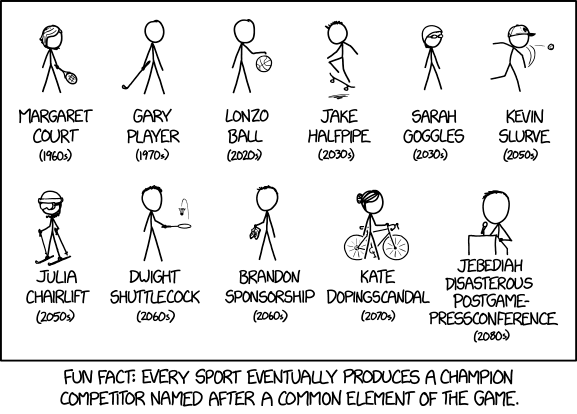
\includegraphics[width=0.5\hsize]{info/xkcd/sports_champions.png}
\end{center}


\subsection{Das Unikino}
Das Unikino ist eine von Studenten geleitete Veranstaltungsreihe, bei der z.B. unbekannte und in Vergessenheit geratene, aber auch recht aktuelle Filme gezeigt werden, oft auch in englischer Originalfassung. Ihr zahlt ihr pro Semester einmalig \EUR{0,30}, eine Vorstellung kostet \EUR{2} Eintritt (übrigens gelten diese Preise auch für Nicht-Studierende!). Alle Filme werden im Hörsaal 24 im Kupferbau gezeigt (Haltestelle Hölderlinstraße, dort direkt an der großen Kreuzung).\\
In den letzten Vorlesungswochen vor der Weihnachtspause wird der Film "` Die Feu\-er\-zang\-en\-bow\-le"' gezeigt. Dieser Film ist nicht nur Kult, die Fachschaft Informatik schenkt bei dieser Vorstellung auch traditionell Glühwein aus. Vorbeischauen lohnt sich also doppelt! Man sollte jedoch bei dieser Vorstellung früh da sein, der Hörsaal ist meistens rappelvoll.

\subsection*{Spielplan}
%Der Standardspieltag ist Dienstag, Filme mit normaler Länge beginnen um 19:45 Uhr, Filme mit Überlänge bereits um 19:15. Beim Wunschfilmabend wählt das Publikum vor der Vorstellung, welcher Film aus einer Auswahl von 5 Filmen gezeigt wird. Der Eintritt pro Film beträgt 2 Euro.  
%\medskip \\
\renewcommand{\arraystretch}{1.2}
\begin{tabular}{l l}
\textbf{Datum} & \textbf{Filmtitel}     			\\
15.10. & Bohemian Rhapsody							\\
22.10. & Free Solo									\\
29.10. & We the Coyotes (franz. Filmtage)			\\
05.11. & The Hate U Give							\\
12.11. & Us											\\
19.11. & Burning									\\
26.11. & Before the Flood (Fridays for Future)		\\
03.12. & Die Feuerzangenbowle						\\
10.12. & Anna and the Apocalypse					\\
07.01. & Shazam!									\\
14.01. & If Beale Street Could Talk					\\
21.01. & Once Upon a Time in Hollywood				\\
28.01. & Shoplifters								\\
04.02. & Instant Family								\\

\end{tabular}

\textbf{Filmbeginn}: 19:45 Uhr, bei Überlänge 19:15 Uhr\\
\textbf{Eintritt}: 2 \euro ~(+0,30 \euro beim ersten Mal)\\
\textbf{Ort}: Hörsaal 24 im Kupferbau\\
Alle Filme in Originalsprache mit Untertiteln\\

Das Programm ist wegen Zeitplanung zu 98 Prozent sicher.
Alle weiteren Infos zum Unikino findet ihr auf \url{https://www.unifilm.de/studentenkinos/tuebingen} oder auch auf Facebook.
% \pagebreak


\subsection{Das Fachsprachenzentrum}
Am Fachsprachenzentrum\footnote{\url{https://www.uni-tuebingen.de/fsz/}} finden semesterbegleitende Kurse und während der Semesterferien zwei- bis vierwöchige Intensivkurse in verschiedenen Sprachen statt.\\	%TODO insert \link{}{}?
Neben den Einsteiger- und Anfängerkursen (UNIcert I/II mit je drei Niveaustufen) kann man auch fachspezifische Kurse belegen z. B. Beruf und Studium, Naturwissenschaften, Wirtschaftswissenschaften, etc.  Ob man direkt mit einer höheren Niveaustufe beginnen darf (oder im Grundkurs beginnen muss) entscheidet ein Einstufungstest vor Ort.  Unterrichtet werden die Kurse meist von Muttersprachlern und haben mittleres bis hohes Niveau.
Die Einschreibung zu den semesterbegleitenden Kursen starten häufig schon vor dem Semester. Die genauen Zeiten werden im Internet (s. o.) bekannt gegeben.  Gerade bei begehrten Kursen (d. h. fast alle Einsteigerkurse wie z. B. Spanisch I oder Italienisch I) sollte man aber bei der  Einschreibung schnell sein. Meist sind alle Plätze schon am ersten Einschreibetag vergeben.\\
Die Kurse sind für Studenten kostenlos. Wer sich angemeldet hat, muss jedoch auch erscheinen, da Anwesenheitspflicht besteht. Ansonsten droht eine Sperre für weitere Kurse am FSZ für das kommende Semester in der jeweiligen Sprache.
  
Eine Alternative zum FSZ der Uni ist natürlich die klassische Volkshochschule. Das Angebot kann auf der Websiete der vhs\footnote{\url{https://www.vhs-tuebingen.de/kurse/sprachen}} eingesehen werden. Dort finden sich Kurse vieler Sprachen, von Englisch bis Hindi oder Suaheli in jeweils mehreren Niveaustufen und mit vielen Spezialkursen, z.B. Konversationskurse, Grammatikkurse, Reisekurse, Kinderkurse. Sie kosten zwischen 90 und 150 EUR (je nach Sprache, Kursart, Dauer, ...) - meistens sind es etwa 90 EUR. Das Niveau dieser Kurse ist im Allgemeinen relativ niedrig, allerdings kann man das auch vorher telefonisch bei der vhs erfragen und sich dort beraten lassen.

\coronabox{Informiere dich bitte auf den entsprechenden Webseiten, ob und wie die Kurse im kommenden Semester stattfinden.}

\vfill


\pagebreak
\section{Die vorlesungsfreie Zeit}
\subsection{Die Klausuren}
\ifinfo
	Die größte Freude der vorlesungsfreien Zeit stellen die Klausuren dar. In ihnen müsst ihr zeigen, was ihr das Semester über gelernt habt. Die Klausuren in Tübingen finden zumeist in der letzten Woche der Vorlesungszeit und der ersten Woche der vorlesungsfreien Zeit statt. Solltet ihr durch eine der Klausuren fallen oder euch entscheiden, dass ihr für eine Klausur noch nicht genug gelernt habt, finden Nachholtermine zu den Klausuren in den letzten beiden Wochen der vorlesungsfreien Zeit statt.\\
Diese Regelung hat den Vorteil, dass ihr in den Semesterferien nur selten Veranstaltungen habt (Die große Ausnahme bilden hier Praktika).\\
\\
Wichtig bei den Klausuren ist, dass ihr euch rechtzeitig dafür anmeldet. Die genauen Anmeldemodalitäten werden euch normalerweise in den ersten Vorlesungen erläutert. Im Zweifel ist es ratsam, seinem Dozierenden rechtzeitig nochmal zu fragen.

\else
	\coronabox{Aufgrund der Corona Pandemie und den einhergehenden Hygiene-Vorschriften, kann über das Format der Klausuren noch nichts gesagt werden, da sich die Regelungen oft ändern. Dies wird dann in den einzelnen Veranstaltungen besprochen. Aktuell wird aus einem gemisch von Präsensklausuren und Onlineklausuren geprüft.} \\
Die größte Freude der vorlesungsfreien Zeit stellen die Klausuren dar. In ihnen müsst ihr zeigen, was ihr das Semester über gelernt habt. Die Klausuren in Tübingen finden zumeist in der letzten Woche der Vorlesungszeit und der ersten Woche der vorlesungsfreien Zeit statt. Solltet ihr durch eine der Klausuren fallen oder euch entscheiden, dass ihr für eine Klausur noch nicht genug gelernt habt, finden Nachholtermine zu den Klausuren in den letzten beiden Wochen der vorlesungsfreien Zeit statt. Ihr könnt euch also bei den meisten Klausuren entscheiden, ob ihr sie zu Beginn oder zum Ende der Ferien schreibt. Aber vorsicht: besteht ihr die Klausur am späteren Termin nicht, könnt ihr sie je nach Vorlesung erst ein Jahr später erneut schreiben.\\
\\
Wichtig bei den Klausuren ist, dass ihr euch rechtzeitig dafür anmeldet. Die genauen Anmeldemodalitäten werden euch normalerweise in den ersten Vorlesungen erläutert. Im Zweifel ist es ratsam, seinen Dozierenden rechtzeitig nochmal zu fragen. Bei den Informatik-Veranstaltungen kann man sich oft in ALMA unter 'Prüfungsverwaltung' oder in der Verwendeten Lehrplattform anmelden. Zu den Psychologie-Klausuren gehen meistens Listen rum und es liegen zusätzlich Anmeldelisten im psychologischen Institut vor dem Büro von Frau Jendreyko.

\fi

\subsection{Das Prüfungsprotokolle-Interface}
Um einen groben Eindruck davon zu bekommen, was einen in den Klausuren und
mündlichen Prüfungen erwartet, verwalten wir das
Pr\"ufungsprotokolleinterface\footnote{\url{https://ppi.fsi.uni-tuebingen.de}}
(PPI).  Dort sammeln wir seit Jahren Ged\"achtnisprotokolle von Prüfungen und
Klausuren.  Damit die gesamte Sammlung aktuell bleibt wäre es gut, wenn ihr
selbst eine heruntergeladen habt, wieder ein Gedächtnisprotokoll hochladet.
Dafür erhaltet ihr dann auch wieder Tokens, die ihr vorher ausgegeben habt. Und
wenn ihr mit anderen zusammenarbeitet bekommt natürlich jeder Tokens.  Die
meisten Grundvorlesungen gibt es netterweise noch ohne Tokens.


\ifinfo
\else
	\vfill
\fi

\ifinfo
	\subsection{Praktika}
	In der vorlesungsfreien Zeit müssen teilweise von Seiten der Universität vorgeschrieben Praktika (Experimentalphysik, Anorganische Chemie, Organische Chemie, Physikalische Chemie, etc.) absolviert werden. Diese sind jedoch abhängig von eurem Studiengang. Ihr solltet daher im verlaufe des ersten Semesters einen Blick in euer Modulhandbuch\footnote{\url{https://uni-tuebingen.de/de/74348}} werfen, um herauszufinden, welche Praktika ihr wann machen müsst.\\

Neben den von der Universität vorgeschrieben Praktika kann es auch sehr sinnvoll sein schonmal das eine oder andere Praktikum in einem Unternehmen zu machen. Viele Arbeitgeber schätzen solche Erfahrungen.

\vfill
\fi

\pagebreak

\section{Universität und Institute}
\subsection{Teile der Universität}
\ifinfo
	\textbf{Morgenstelle}\\
Auf der Morgenstelle befindet sich das Hörsaalzentrum, das Gebäude der Universität, welches sowohl die meisten als auch die größten Hörsäle beherbergt. Hier werdet ihr unter anderem auch die meisten eurer Grundvorlesungen haben.\\
Die Morgenstelle erreicht man am bequemsten mit dem Bus. In 98\% der Fälle solltet ihr an der Haltestelle \emph{BG Unfallklinik} aussteigen. Die anderen Haltestellen \emph{Auf der Morgenstelle} und \emph{Botanischer Garten} eignen sich nur, wenn ihr z.B. in N10 oder N11 müsst.\\ Bei den Hochhäusern auf der Morgenstelle gilt: Jedes Gebäude besitzt einen Buchstaben, der außen am Gebäude angebracht ist.  Die Raumnummern orientieren sich an den Gebäudebuchstaben und Stockwerken, z.B. befindet sich der Raum C9A03 im C-Bau im 9. Stockwerk.\footnote{Im Gegensatz dazu ist der Raum 7E02 NICHT im E-Bau im 7. Stockwerk. Achtet auf die Reihenfolge!} Wenn ihr Gebäude C und D betretet, befindet ihr euch bereits im dritten Stockwerk. Wichtig sind im C-Bau vor allem die Poolräume, welche sich im zweiten Stockwerk links vom Aufzug befinden. \\
%TODO Orientierung Morgenstelle
%Einen Lageplan der wichtigen Gebäude und wichtigsten Orte auf der Morgenstelle findet ihr im Anhang.

\textbf{Sand}\\
Das Wilhelm-Schickard-Institut für Informatik oder auch einfach nur Sand genannt\footnote{Basierend auf den Postadressen Sand 1, 6, 7, 8, 13 und 14} ist das Institut der Informatik in Tübingen. In den ersten Semestern werdet ihr hier höchstens die Fachschaft besuchen. Auch wenn das Institut etwas außerhalb der restlichen Universität liegt, besticht es dennoch durch sein großzügiges Platzangebot und zahlreiche Möglichkeiten zur Freizeitgestaltung in Pausen. Unter anderem befinden sich auf dem Gelände ein Volleyballfeld, ein Fußballfeld und eine Tischtennisplatte. Bälle und Tischtennisschläger liegen in unserem Fachschaftsraum und dürfen von allen Studierenden der Informatik ausgeliehen werden.\\
Da es auf dem Sand anfangs immer schwierig ist, sich bei den Raumbezeichnungen zurechtzufinden, haben wir einen kleinen Übersichtsplan pro Stockwerk erstellt. Ihr findet diesen im Anhang.
%TODO Orientierung Sand

\textbf{TTR\footnote{aka: Die Machine von Learning-Straße}}\\
Beginnend mit dem Tübingen AI Research Building wird für die Informatik auf der Oberen Viehweide mehr Platz geschaffen. Wer also Professoren für Machine Learning und Computergrafik sucht wird dort fündig.

\textbf{Uni Tal}\\
Ein großer, wenn auch für die Informatik eher irrelevanter Teil der Universität, liegt an der Wilhelmstraße, dem sogenannten Tal. Als Informatiker hat man hier höchstens Nebenfachveranstaltungen.
\vfill

\else
	\textbf{Morgenstelle}\\
Auf der Morgenstelle befindet sich das Hörsaalzentrum, das Gebäude der Universität, welches sowohl die meisten als auch die größten Hörsäle beherbergt. Hier werdet ihr unter anderem auch die meisten eurer Grundvorlesungen haben.\\
Die Morgenstelle erreicht man am bequemsten mit dem Bus. In 98\% der Fälle solltet ihr an der Haltestelle \emph{BG Unfallklinik} aussteigen. Die anderen Haltestellen \emph{Auf der Morgenstelle} und \emph{Botanischer Garten} eignen sich nur, wenn ihr z.B. in N10 oder N11 müsst.\\ Bei den Hochhäusern auf der Morgenstelle gilt: Jedes Gebäude besitzt einen Buchstaben, der in mehr oder weniger gut sichtbarem Orange außen am Gebäude angebracht ist.  Die Raumnummern orientieren sich an den Gebäudebuchstaben und Stockwerken, z.B. befindet sich der Raum C9A03 im C-Bau im 9. Stockwerk.\footnote{Im Gegensatz dazu ist der Raum 7E02 NICHT im E-Bau im 7. Stockwerk. Achtet auf die Reihenfolge!} Wenn ihr Gebäude C und D betretet, befindet ihr euch bereits im dritten Stockwerk. Warum man sich das so ausgedacht hat, wissen wir auch nicht. Wichtig sind im C-Bau vor allem die Poolräume, welche sich im zweiten Stockwerk links vom Aufzug befinden.

\textbf{Sand}\\
Das Wilhelm-Schickard-Institut für Informatik oder auch einfach nur Sand genannt ist das Institut der Informatik in Tübingen. Auch wenn das Institut etwas außerhalb der restlichen Universität liegt, besticht es durch sein großzügiges Platzangebot und zahlreiche Möglichkeiten zur Freizeitgestaltung in Pausen. Unter anderem befinden sich auf dem Gelände ein Volleyballfeld, ein Fußballfeld und eine Tischtennisplatte. Bälle und Tischtennisschläger liegen im Fachschaftsraum der Fachschaft Informatik und dürfen gerne ausgeliehen werden. Es gibt keine Mensa, jedoch fährt ein bis zwei mal in der Woche ein Foodtruck zum Sand.\\

\textbf{Psychologisches Institut}\\
Das Psychologische Institut (PI) ist wie der Name schon sagt das Institut der Psychologen. In ihm befindet sich auch der Hörsaal in dem ihr die Vorlesung ''Einführung in die Kognitionswissenschaft'' haben werdet. Außerdem finden hier viele Versuche statt. Manchmal wird das Gebäude auch auf Grund seiner früheren Verwendung \textit{Alte Frauenklinik} genannt.

\textbf{Kupferbau}\\
Der Kupferbau ist das Hörsaalzentrum im Tal. In ihm befinden sich mehrere größere Hörsäle. Hier werdet ihr unter anderem die Vorlesung ''Allgemeine Psychologie A'' haben.

\textbf{Neue Aula}\\
Die neue Aula im Tal ist mit den beiden Brunnen das Vorzeigegebäude der Uni. Hier finden vor allem Jura-Vorlesungen statt, jedoch wird der Hörsaal Audimax sowie der Festsaal (bei im ersten Stock) gerne für größere Veranstaltungen verwendet.

\vfill
\fi

\subsection{Was ist wo?}
\ifinfo
	\subsubsection*{Studierendensekretariat}
Das Studierendensekretariat\footnote{\url{https://uni-tuebingen.de/de/596}} befindet sich in der Wilhelmstraße 11 direkt neben der Mensa Wilhelmstraße. Das Studierendensekretariat ist zuständig für eure Immatrikulation und Exmatrikulation, amtliche Bescheinigungen, die TAN-Listen fürs Campus sowie alles, was mit dem Studierendenausweis zu tun hat.

\subsubsection*{Studierendenterminals}
An den Studierendenterminals könnt ihr den Aufdruck auf eurem
Studierendenausweis aktualisieren. Dies solltet ihr nach erfolgreicher Rückmeldung schleunigst tun, oft wird beim Kauf des Semestertickets ein aktueller Aufdruck erwartet, außerdem müsst ihr sonst in den Mensen
den vollen Gästepreis zahlen!\\
Momentan gibt es drei Terminalgruppen:\\
Eine auf der Morgenstelle im Hörsaalzentrum in der Nähe der Herrentoilette,
eine im Studentensekretariat in der Wilhelmstraße und eine bei den Kopierern in der UB.

\subsubsection*{Prüfungssekretariate}
Das Prüfungssekretariat ist zuständig für alle möglichen Prüfungsangelegenheiten. Hier könnt ihr euch im Zweifelsfall für Klausuren an- und abmelden, sollte dies aus irgendwelchen Gründen über das Campus nicht möglich sein. Für die Informatiker befinden sich alle Prüfungssekretariate auf dem Sand.\\
Je nach Studiengang ist ein anderes Prüfungssekretariat für euch zuständig. Ihr findet euer entsprechendes Sekretariat im Hilfe-Abschnitt. Meistens können Formulare, anstatt die Sprechzeiten in Anspruch zu nehmen, auch unkompliziert in das entsprechende Postfach eingeworfen werden.

%\textbf{Wichtig:} Ihr müsst euch zu Beginn eures Studium nochmal extra in eurem Prüfungssekretariat anmelden, damit eure erbrachten Leistungen verbucht werden können. Hierfür liegt vor den Sekretariaten ein spezielles Formular aus. Erst wenn ihr diese Anmeldung getätigt habt, könnt ihr überhaupt Prüfungen mitschreiben! 
\vfill \pagebreak 
\subsubsection*{Computer Pools}
Räume mit für Studierende zugänglichen Computern befinden sich sowohl auf der Morgenstelle (Untergeschoss des C-Bau) als auch auf dem Sand (in den Räumen B033 und C119). Auf den Rechnern in diesen Räumen könnt ihr euch mit eurer ZDV-Kennung und Passwort unkompliziert anmelden. Eure ZDV-Kennung (\texttt{zx[…]}) braucht ihr für beinahe jeden Rechner der Uni, es empfiehlt sich also, diese auswendig zu lernen. 

\subsubsection*{Bibliotheken}
\textbf{DIE} Bibliothek der Universität ist die
Universitätsbibliothek (UB).  Im Informationsheft der ZV sind
sämtliche ihrer Einrichtungen auf\-ge\-führt.  Sie hat
allerdings den Nachteil, dass sie die einzelnen Fachbereiche nicht so
detailliert abdecken kann, wie es manchmal wünschenswert wäre,
denn dafür sind die Fach-Bibliotheken der einzelnen Fakultäten
zuständig.  Aber mit etwas Aufwand kann über die UB fast jedes Buch
(auch per Fernausleihe) besorgt werden -- Fragen schadet nie!
%\pagebreak

\begin{center}

\includegraphics[width=0.45\hsize]{info/xkcd/books_toomany.png}
\end{center}

Für die Informatik sind vorwiegend vier Bibliotheken interessant:
\begin{description}
	\item[Hauptstelle der Unibibliothek] Zwar sind hier nicht eure wichtigsten
	Bücher untergebracht, aber im neuen Ammer-Bau lässt es sich prima
	lernen. Es gibt zahlreiche Arbeitsplätze und Arbeitsräume, die
	allerdings schnell belegt sind. Außerdem findet man hier immer die
	aktuellsten Tageszeitungen und einige Rechnerpools.
	Grade in den ersten Tagen eures Studiums ist ein Besuch der Hauptstelle
	sehr zu empfehlen, da zu Beginn des Semesters täglich Einführungen in den Umgang mit der UB stattfinden. Zusätzlich gibt es viele hilfreiche Tricks für das tägliche Leben mit der UB. Wann diese Führungen angeboten werden, erfahrt ihr unter  \url{https://www.ub.uni-tuebingen.de/}. Wichtig sind die extrem langen Ausleihfristen: die Standardfrist von 4 Wochen verlängert sich automatisch auf bis zu 3 Monate, falls euer Buch nicht angefordert wird. Dafür solltet ihr den EMail - Alarm anschalten, damit ihr auch bei Abwesenheit aus Tübingen über Rückgabefristen informiert bleibt. 
	
	\item[Außenstelle der Uni-Bibliothek auf der Morgenstelle]
	Hier findet ihr eigentlich alles, was ihr im Grundstudium an
	Literatur braucht.  Was nicht in den Regalen steht, könnt ihr
	im Normalfall bestellen.  Die meisten der dort stehenden Bücher könnt ihr
	ausleihen. Den dazu benötigten Ausweis besitzt ihr in Form eures Studentenausweises bereits.
	
	\item[Mathe-Bibliothek]
	Das ist die Fachbibliothek der Fakultät für Mathematik.  Sie
	befindet sich im C-Gebäude auf dem 4. Stock (vom
	Hörsaalzentrum aus kommt man schon im 3. Stock in das
	C-Gebäude!). Einige Bücher können ausgeliehen werden,
	andere sind nur Präsenzbestand.  Außerdem steht da ein Regal
	mit Informatik-Büchern und Skripten, die z.T. ganz
	interessant sind (gleich links vom Eingang).  Auch finden sich
	hier die sog. Hand-Apparate zu den Vorlesungen (nach dem
	Eingang rechts und dann ganz nach hinten).  Dies sind
	Zusammenstellungen von Büchern, die ein Prof. zu seiner
	Vorlesung empfiehlt.  Diese Bibliothek ist besonders
	interessant, weil hier in Ruhe gearbeitet werden kann.
	Außerdem gibt es einen Kopierer in dieser Bibliothek (linke
	Seite) und zwei kleine Arbeitsräume mit Tafeln aber ohne
	Tageslicht (rechte Seite).  Diese sind für Gruppenarbeiten
	genauso geeignet, wie die Tische und Bänke, die vor der
	Mathe-Bib aufgestellt sind.
	
	\item[Info-Bibliothek]
	Die Fachbibliothek der Informatik befindet sich auf dem Sand
	im ersten Stockwerk.  Die Bücher dort sind eigentlich erst in
	späteren Semestern interessant.  Aller\-dings steht sie für jeden
	offen, der sich jetzt schon dafür interessiert.  "`Steht
	offen"' ist allerdings mit Vorsicht zu genießen, da die
	Bibliothek nicht immer geöffnet ist (Die aktuellen Zeiten
	sind an der Bib angeschlagen, %meistens ist sie aber
	%zwischen 13 und 18 Uhr offen). Seit Beginn des Sommersemesters 2006 sind die
	%Öffnungszeiten versuchsweise auf 10 bis 18 Uhr verlängert worden.
	momentan ist die Bib auf dem Sand lediglich von 14 bis 17 Uhr geöffnet.
	In den Semesterferien ist mit unregelmäßigen, reduzierten Besuchszeiten zu rechnen, manchmal wird die Bib über die Semesterferien auch komplett geschlossen!
	
	Ebenfalls interessant ist die umfangreiche Zeitschriftensammlung,
	die eigentlich alle wichtigen Zeitschriften im
	Informatik-Bereich umfasst.
	
	Für euch sind zunächst insbesondere die Klausuren der
	vergangenen Jahre wichtig, welche im zweiten Raum links (der mit
	der großen Metallschiebetür) auf der linken Seite in Ordnern gesammelt
	werden.  Nach Absprache mit der Aufsicht solltet ihr euch vor den
	Prüfungen einige Klausuren zur Übung kopieren.
	
	Sämtliche vorhandene Medien sind Präsenzbestand. Bücher können
	jedoch über Nacht oder über das Wochenende ausgeliehen werden, wenn ein Ausweis
	(egal welcher) da gelassen wird.
	
	Weitere Informationen findet ihr unter \url{https://www.wsi.uni-tuebingen.de/bibliothek.html}
	
\end{description}

Wenn ihr nicht gerade eine Gruppenarbeit erledigen müsst, so sind die
Bibliotheken eigentlich sehr gute Plätze zum Arbeiten.  So hat man
auch die Bücher direkt vor Ort und es besteht kein Bedarf sie
auszuleihen.  Deshalb ist zum Beispiel die Info-Bib auch eine
Präsenzbibliothek, was bedeutet, dass man normalerweise als
Studierender Bücher nicht für länger ausleihen darf.


\else
	\subsubsection*{Studierendensekretariat}
Das Studierendensekretariat\footnote{\url{https://uni-tuebingen.de/de/596}} befindet sich in der Wilhelmstraße 11 direkt neben der Mensa Wilhelmstraße. Das Studierendensekretariat ist zuständig für eure Immatrikulation und Exmatrikulation, amtliche Bescheinigungen, die TAN-Listen fürs Campus sowie alles, was mit dem Studierendenausweis zu tun hat.	%TODO insert \link{}{}?

\subsubsection*{Studierendenterminals}
An den Studierendenterminals könnt ihr den Aufdruck auf eurem
Studierendenausweis aktualisieren. Dies solltet ihr nach erfolgreicher Rückmeldung schleunigst tun, oft wird beim Kauf des Semestertickets ein aktueller Aufdruck erwartet, außerdem müsst ihr sonst in den Mensen
den vollen Gästepreis zahlen!\\
Momentan gibt es drei Terminalgruppen:\\
Eine auf der Morgenstelle im Hörsaalzentrum in der Nähe der Herrentoilette,
eine im Studentensekretariat in der Wilhelmstraße und eine bei den Kopierern in der UB.

\subsubsection*{CIP Pools}
Räume mit für Studierende zugänglichen Computern befinden sich sowohl auf der Morgenstelle (Untergeschoss des C-Bau) als auch auf dem Sand (in den Räumen B033 und C119). Auf den Rechnern in diesen Räumen könnt ihr euch mit eurer ZDV-Kennung und Passwort unkompliziert anmelden.

\subsubsection*{Bibliotheken}
\textbf{DIE} Bibliothek der Universität ist die
Universitätsbibliothek (UB).  Im Informationsheft der ZV sind
sämtliche ihrer Einrichtungen auf\-ge\-führt.  Sie hat
allerdings den Nachteil, dass sie die einzelnen Fachbereiche nicht so
detailliert abdecken kann, wie es manchmal wünschenswert wäre,
denn dafür sind die Fach-Bibliotheken der einzelnen Fakultäten
zuständig.  Aber mit etwas Aufwand kann über die UB fast jedes Buch
(auch per Fernausleihe) besorgt werden -- Fragen schadet nie!
%\pagebreak
\begin{center}

\includegraphics[width=0.45\hsize]{info/xkcd/books_toomany.png}
\end{center}

\vfill
%\pagebreak

Für die Kognitionswissenschaft sind folgende Bibliotheken interessant:
\begin{description}
	\item[Hauptstelle der Unibibliothek] Zwar sind hier nicht eure wichtigsten
	Bücher untergebracht, aber im neuen Ammer-Bau lässt es sich prima
	lernen. Es gibt zahlreiche Arbeitsplätze und Arbeitsräume, die
	allerdings schnell belegt sind. Außerdem findet man hier immer die
	aktuellsten Tageszeitungen und einige Rechnerpools.
	Grade in den ersten Tagen eures Studiums ist ein Besuch der Hauptstelle
	sehr zu empfehlen, da zu Beginn des Semesters täglich Einführungen in den Umgang mit der UB stattfinden. Zusätzlich gibt es viele hilfreiche Tricks für das tägliche Leben mit der UB. Wann diese Führungen angeboten werden, erfahrt ihr unter  \url{http://www.ub.uni-tuebingen.de/}. Wichtig sind die extrem langen Ausleihfristen: die Standardfrist von 4 Wochen verlängert sich automatisch auf bis zu 3 Monate, falls euer Buch nicht angefordert wird. Dafür solltet ihr den EMail - Alarm anschalten, damit ihr auch bei Abwesenheit aus Tübingen über Rückgabefristen informiert bleibt. 
	
	\item[Außenstelle der Uni-Bibliothek auf der Morgenstelle]
	Hier findet ihr eigentlich alles, was ihr im Grundstudium an
	Literatur braucht.  Was nicht in den Regalen steht, könnt ihr
	im Normalfall bestellen.  Die meisten der dort stehenden Bücher könnt ihr
	ausleihen. Den dazu benötigten Ausweis besitzt ihr in Form eures Studentenausweises bereits.
	
	\item[Mathe-Bibliothek auf der Morgenstelle]
	Das ist die Fachbibliothek der Fakultät für Mathematik. Sie
	befindet sich im C-Gebäude auf dem 4. Stock (vom
	Hörsaalzentrum aus kommt man schon im 3. Stock in das
	C-Gebäude!). Einige Bücher können ausgeliehen werden,
	andere sind nur Präsenzbestand.  Außerdem steht da ein Regal
	mit Informatik-Büchern und Skripten, die z.T. ganz
	interessant sind (gleich links vom Eingang).  Auch finden sich
	hier die sog. Hand-Apparate zu den Vorlesungen (nach dem
	Eingang rechts und dann ganz nach hinten).  Dies sind
	Zusammenstellungen von Büchern, die ein Prof. zu seiner
	Vorlesung empfiehlt.  Diese Bibliothek ist besonders
	interessant, weil hier in Ruhe gearbeitet werden kann.
	Außerdem gibt es einen Kopierer in dieser Bibliothek (linke
	Seite) und zwei kleine Arbeitsräume mit Tafeln aber ohne
	Tageslicht (rechte Seite).  Diese sind für Gruppenarbeiten
	genauso geeignet, wie die Tische und Bänke, die vor der
	Mathe-Bib aufgestellt sind.
	
	\item[Informatik-Bibliothek auf dem Sand]
	Die Fachbibliothek der Informatik befindet sich auf dem Sand
	im ersten Stockwerk.  Die Bücher dort sind eigentlich erst in
	späteren Semestern interessant.  Allerdings steht sie für jeden
	offen, der sich jetzt schon dafür interessiert.  "`Steht
	offen"' ist allerdings mit Vorsicht zu genießen, da die
	Bibliothek nicht immer geöffnet ist. Die aktuellen Zeiten
	sind an der Bib angeschlagen, momentan ist die Bib auf dem Sand lediglich von 14 bis 17 Uhr geöffnet.
	In den Semesterferien ist mit unregelmäßigen, reduzierten Besuchszeiten zu rechnen, manchmal wird die Bib über die Semesterferien auch komplett geschlossen!
	
	Ebenfalls interessant ist die umfangreiche Zeitschriftensammlung,
	die eigentlich alle wichtigen Zeitschriften im
	Informatik-Bereich umfasst.
	
	Für euch sind zunächst insbesondere die Klausuren der
	vergangenen Jahre wichtig, welche im zweiten Raum links (der mit
	der großen Metallschiebetür) auf der linken Seite in Ordnern gesammelt
	werden.  Nach Absprache mit der Aufsicht solltet ihr euch vor den
	Prüfungen einige Klausuren zur Übung kopieren.
	
	Sämtliche vorhandene Medien sind Präsenzbestand. Bücher können
	jedoch über Nacht oder über das Wochenende ausgeliehen werden, wenn ein Ausweis	(egal welcher) da gelassen wird.
	
	Weitere Informationen findet ihr unter \url{http://bib.informatik.uni-tuebingen.de}	%TODO insert \link{}{}?
	
	\item[Psychologie-Bibliothek im PI]
Im Untergeschoss des Psychologischen Instituts befindet sich die Psychologie-Bibliothek. Dort findet ihr viele Kogni-relevante Bücher und Kopiervorlagen für die Bücher der Psychologie-Vorlesungen. Außerdem erhaltet ihr dort eure Versuchspersonen-Bescheinigungen.
	
\end{description}

Wenn ihr nicht gerade eine Gruppenarbeit erledigen müsst, so sind die
Bibliotheken eigentlich sehr gute Plätze zum Arbeiten.  So hat man
auch die Bücher direkt vor Ort und es besteht kein Bedarf sie
auszuleihen.  Deshalb ist zum Beispiel die Info-Bib auch eine
Präsenzbibliothek, was bedeutet, dass man normalerweise als
Studierender Bücher nicht für länger ausleihen darf.



\fi

\pagebreak
\subsection{PCs, Mail etc.}
	% infra/zdv.tex
Jeder Student der Universität Tübingen hat bei seiner Immatrikulation einen ZDV-Account erhalten (meist in der Form zxabc12), der in den Poolräumen der Uni, zur Authentifizierung im WLAN-Netz und für diverse andere Dienste kostenlos benutzt werden kann. 

% \coronabox{Wie bei allem gerade lässt sich nicht sagen, inwieweit die Pool-Räume zur Verfügung stehen.}
\begin{description}

  \item[Drucker and friends:]
    Gedruckt wird auf Laserdruckern der Firma Morgenstern, an denen man mit dem Studentenausweis bezahlt. Kosten pro S/W-Seite:
    3 Cent.

  \item[EMail:]
    Ein Viren-gefilterter (lässt sich nicht abstellen) und SPAM-gefilterter
    (abschaltbar) E-Mail-Account \email{vorname.nachname@student.uni-tuebingen.de},
    der per IMAP sowohl an der Uni als auch Zuhause nutzbar ist. Webmail ist unter \url{https://webmail.uni-tuebingen.de/} verfügbar. 

  \item[Pools:] ~\\
    \begin{tabular}{ll}
      Wilhelmstr. 106 / Wächterstr. 76 &                SUSE-Linux, Windows \\
      Morgenstelle C-Bau, 2. Stock &            SUSE-Linux, Windows \\
    \end{tabular}

    Die Website des ZDV bietet hierzu auch eine Übersichtskarte
    \footnote{\url{https://uni-tuebingen.de/de/1711}}.	%TODO insert \link{}{}?
    Wichtig: Ihr benötigt euren Studentenausweis, um in der Wilhelmstraße in das Gebäude zu kommen \emph{und} um wieder raus zu kommen! Dafür kommt ihr von 7 Uhr morgens bis 4 Uhr nachts ins Gebäude. Offiziell ist es nicht erlaubt, für jemanden die Tür offen zu halten\footnote{Ansonsten droht die Sperrung des Accounts}, jeder sollte also mit seinem eigenen Ausweis einzeln durch die Türen gehen. Auf der Morgenstelle gelten die Gebäudeöffnungszeiten.

  \item[Kurse:]
    Das ZDV bietet einige Kurse, die z.T. sehr nützlich sind. Z.B. \LaTeX,
    Unix-Ein\-führ\-ung, C-Programmieren, MATLAB ... Nähere Infos erhaltet ihr im
    WWW, per allgemeiner ZDV-Rundmail oder durch Aushänge.

   
   \item[Windows \& Office für Bildung] Nicht direkt ein Service des ZDV, aber vielleicht trotzdem interessant: Es existiert eine kostenlose Möglichkeit, als Student ein Office 365-Abo und Windows 10 Edu zu erwerben. Nachteil: Man muss ein separates Konto bei Microsoft anlegen. Weitere Infos hierzu findet ihr unter \url{https://uni-tuebingen.de/de/45057}.	%TODO insert \link{}{}?


  \item[Bildungslizenzen] Auf der Software Übersichtsseite \footnote{\url{https://uni-tuebingen.de/de/77076}} kann man sich durch die verschieden Software Lizenzen klicken, die auch Studierenden kostenlos zur Verfügung stehen.

  \item[Ansprechpartner Pools:]
    Ist erreichbar unter \email{beratung@zdv.uni-tuebingen.de}.
    %\footnote{siehe auch \url{http://www.zdv.uni-tuebingen.de/kontakt-antraege-beratung.html}}.

	
\end{description}

\subsection{WLAN-Zugang mit eduroam}
	Eduroam ermöglicht es euch, europaweit an verschiedenen teilnehmenden
Universitäten\footnote{Deutschland-Karte:
\url{https://map.eduroam.de/leaflet/eduroam/eduroam-map.html}} die Zugangsdaten
deiner eigenen Uni zu benutzen, um ins Internet zu kommen. Dass eine Uni oder
FH bei Eduroam mitmacht, bekommt ihr i.\,d.\,R. relativ schnell mit, sobald ihr
euer Smartphone in die Hand nehmt.

\subsection*{Zertifikat}
  Um zu verhindern, dass jemand irgendwo ein WLAN-Netz mit dem Namen eduroam
  eröffnet und eure Daten abgreift, müsst ihr unbedingt das Zertifikat
  überprüfen\footnote{Genau genommen prüfen wir den Zertifizierungspfad mit dem
  Wurzelzertifikat der Deutschen Telekom.}. Dieser Schritt ist leider etwas
  umständlich, sollte aber auf keinen Fall weggelassen werden! Ihr braucht dazu das Wurzelzertifikat \glqq\texttt{T-Telesec Global Root Class 2}\grqq. Dies
  sollte schon vorhanden sein (v.\,a. unter GNU/Linux und Windows), kann
  jedoch unter Android nicht für W-LAN verwendet werden. Außerdem ist unter iOS
  und OS X laut ZDV eine manuelle Konfiguration nicht möglich, es muss also das
  Konfigurationsprofil vom ZDV verwendet werden
  \footnote{\url{https://www.uni-tuebingen.de/fileadmin/Uni_Tuebingen/Einrichtungen/ZDV/Dokumente/Anleitungen/eduroam/eduroam-uni-tuebingen.mobileconfig}},
  welches das Zertifikat bereits beinhaltet.

\subsection*{Konfiguration}
  Am besten folgt man einer der ausführlichen und plattformspezifischen
  Anleitungen vom ZDV:
  \url{https://uni-tuebingen.de/de/13958}.\\
  Als fortgeschrittene Variante kann man unter GNU/Linux \texttt{netctl} oder auch
  direkt \texttt{wpa\_supplicant} verwenden. Anleitungen dazu findet man im
  \texttt{configs}-Repo der Fachschaft
  (\url{https://github.com/fsi-tue/configs/tree/master/eduroam}).

\subsection*{Authentifizierung}
  Um zu gewährleisten, dass der Zugang überall funktioniert, muss man sich an
  folgende Konvention halten (bitte beachtet, dass hier kein
  \emph{@student.uni-tuebingen.de} verwendet werden darf): \medskip \\
  \begin{tabular}{l|l}
    Benutzername (Identität) & <zx-Kürzel>@uni-tuebingen.de \\ \hline
    Passwort                 & <ZDV-Passwort>
  \end{tabular}

\vfill


\section{Tübingen - mehr als eine Universität}
\subsection{Wohnen}
Wohnen in Tübingen ist ein großes Thema.  Wohnheime werden von verschiedenen Institutionen betrieben: Studentenwerk AdöR, Tübinger Studentenwerk eV, einigen christlichen Vereinigungen und sonstigen Vereinen. 

Private Angebote kann man über \url{https://www.wg-gesucht.de} und \url{https://www.housinganywhere.com} finden.	%TODO insert \link{}{}?	 %TODO insert \link{}{}?

Die Wohnungspreise in Tübingen sind allgemein relativ hoch. Hierbei kommt es selbstverständlich auf die Lage und den Vermieter an. Die Wohnheimplätze sind im Vergleich zu vielen privaten "`Wohn-Angeboten"' etwas günstiger.  Euer ganzes Studi-Leben könnt ihr jedoch nicht im selben Wohnheim verbringen, denn üblicherweise setzen die Träger Fristen von 4 bis 6 Semestern.

% Comment: Was part of Mensa Wilhelmstraße
% Bei der Suche nach einem Zimmer oder einer Wohnung bei privaten Vermietern kann die Zimmervermittlung des Studierendenwerks\footnote{\url{https://www.my-stuwe.de/wohnen/privatzimmervermittlung/}} helfen. Darüber hinaus finden sich in den Mittwochs und Samstagsausgaben des Schwäbischen Tagblatts auch immer wieder Zimmerangebote. Alternativ kann man auch selbest eine eigene Anzeige schalten.

In der Mensa Shedhalle und der Mensa Morgenstelle liegt (kostenlos!) das \emph{Dschungelbuch} aus, das u.a. Informationen zu den Wohnheimen enthält. Sehr empfehlenswert!

Kurzfristig eignet sich auch die Jugendherberge in der Gartenstraße 22, Tel: 07071/23002


\subsection{Verkehr}
Die Hauptfortbewegungsarten in Tübingen sind zu Fuß, per Fahrrad oder dem Bus, da in Tübingen alles nicht weit entfernt ist. Wer sehr sportlich ist kommt mit Fuß und Fahrrad auch zum Sand oder zur Morgenstelle. Da Tübingen jedoch sehr hügelig ist\footnote{\url{https://youtu.be/5xBSrqpiiCk}}, empfiehlt es sich für Normalsterbliche, ein Semesterticket zu erwerben.	%TODO insert \link{}{}?
\vfill \pagebreak
\subsubsection*{Mit dem Bus}
Die günstigste Art die Tübinger Busse zu nutzen ist, sich ein Semesterticket zu kaufen. Man zahlt zu Beginn des Semesters \Ticketpreis (der Rest ist im Sozialbeitrag enthalten, den ihr an das Studentenwerk entrichten müsst).  Damit kann man dann innerhalb des \emph{Naldo-Bereichs}, das sind die Landkreise Tübingen, Reutlingen, Zollern-Alb sowie Sigmaringen (und einzelne Strecken in angrenzenden Landkreisen), alle öffentlichen Verkehrsmittel benutzen. Dazu zählen sowohl die Stadtbusse aller genannten Städte, als auch sämtliche Züge (außer IC) und Regionalbusse, die in dieser Region fahren.

Das Ticket bekommt ihr unter anderem in den Reisezentren in Reutlingen und Tübingen sowie in der Touristeninformation Tübingens an der Neckarbrücke. Zum Kauf müsst ihr euren Studentenausweis und den kleinen Abschnitt "`Bescheinigung für das Semesterticket"' des großen Bescheinigungsbogens mitbringen, der euch nach der Einschreibung per Post zugeschickt wurde.

Seit dem Wintersemester 2014/2015 gilt außerdem die Freizeitregelung von Naldo. Damit könnt ihr unter der Woche ab 19 Uhr und am Wochenende ganztägig Busse und Bahnen innerhalb des Naldo-Gebiets kostenlos nutzen. Dafür braucht ihr einfach nur euren Studentenausweis mit dem Naldo-Logo darauf. Falls ihr also nur abends und/oder am Wochenende auf den Bus angewiesen seid, könnt ihr euch u.U. den Anschaffungspreis für das Semesterticket sparen.
Zusätzlich gilt im Tübingen seit Februar 2018 der \emph{ticketfreie Samstag}. Will heißen: Ihr könnt von Freitag Mitternacht bis Sonntag früh um 5 Uhr alle Busse im Tübinger Stadtgebiet kostenfrei nutzen. Dies ist vor allem praktisch für Freunde und Eltern, die euch in Tübingen besuchen und keinen Studentenausweis mit naldo-Logo besitzen. Kostenfrei sind Samstags ebenfalls die Nachtbusse und die Linien nach Hirschau und Bühl, aber nicht die regionalen Buslinien nach Kusterdingen, Reutlingen oder Mössingen. 

Sehr attraktiv sind auch die Donnerstag- (Clubhaus!), Freitag- und Samstag Nacht bis ca. 4.30 Uhr verkehrende Nachtbusse.  Die Takte sind hier zwar nur (halb-)stündlich und die Fahrt dauert vielleicht etwas länger als normal, aber Mensch kommt sicher Heim (egal, in welchem Zustand).  Also noch ein Grund, das Semesterticket zu erwerben, da es auch für die Nachtbusse gilt. An den anderen Tagen fährt der Nachtbus bis ca. 3 Uhr.

\begin{center}
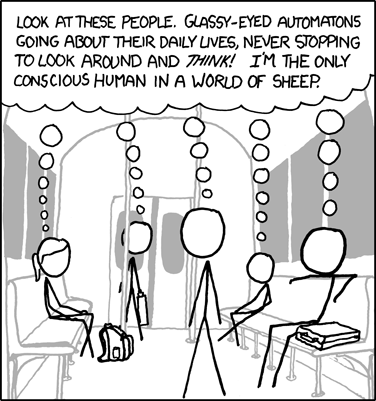
\includegraphics[width=0.5\hsize]{info/xkcd/sheeple.png}
\end{center}

\subsubsection*{Mit dem Fahrrad}
Wie in den meisten Unistädten wird in Tübingen sehr viel Fahrrad gefahren. Es gibt daher auch vor allen wichtigen Gebäuden die Möglichkeit sein Fahrrad anzuschließen. Darüber kann das Fahrrad im Bus die steilen Anstiege mitgenommen werden (zumindest wenn nicht gerade Sperrzeit ist, in vielen Bussen befindet sich dazu ein Aushang).

\subsubsection*{Zu Fuß}
Wie bereits erwähnt sind die meisten Wege in Tübingen sehr kurz, sodass man selten mehr als eine halbe Stunde laufen muss, um sein Ziel zu erreichen. Dies ist vor allem praktisch, wenn das Rad mal wieder einen Platten hat oder man den letzten Bus verpasst hat.

\subsubsection*{Die SAMs}
Ist der Weg doch mal zu weit oder die Füße zu müde gibt es noch die Möglichkeit ein SAM (\textbf{S}ammel\textbf{a}nruf
\textbf{M}ietfahrzeug) zu rufen. Gerade wenn man in einem der ausgelagerten Vororte von Tübingen, wie Hirschau,
Weilheim, Unterjesingen, ..., wohnt ist dies sehr praktisch. Das SAM bringt euch von Haustür evtl. über Umwege zu Haustür (in der Innenstadt nur von/zu bestimmten SAM-Treffpunkten).

\subsubsection*{Mit dem Auto}
Wer trotz dieses guten Angebots an Nahverkehrsmittel mit dem Auto kommen will/muss, sollte folgendes beachten: Kostenlose Parkplätze gibt es nur auf dem Sand, nicht auf der Morgenstelle.  Dort benötigt man für den studentischen Parkplatz eine Nutzungsberechtigung, die man aber nur erhält, wenn die Fahrzeit mit Bus und Bahn länger als 40 Minuten dauern würde (Inwieweit es hier für Informatikstudenten Ausnahmen gibt, ist derzeit unklar), außerdem ist die Anzahl an Parkplätzen sehr begrenzt.

 Erledigen könnt ihr die Freischaltung in dem Büro schräg gegenüber dem Studententerminal im Hörsaalzentrum (direkt neben dem Ausgang Richtung Neubau Chemie). Ihr müsst dafür aber unbedingt das Datenkontrollblatt mitbringen, welches euch per Post zugeschickt wurde. Für alle anderen mit kürzerer Fahrzeit steht oberhalb der Morgenstelle ein kostenpflichtiges Parkhaus zur Verfügung. Wenn ihr eine Parkkarte für das ganze Semester kauft, wird's deutlich günstiger. Infos zu den Tarifen des Parkhauses findet ihr unter \url{https://www.pbw.de/?cmd=Dauerparker&id_city=11&id_object=58}.

\subsubsection*{Von und nach Tübingen}
Wer nach Tübingen oder von Tübingen wegfährt, kann dies gut mit Auto, Bahn oder Fernbus. Züge fahren fast stündlich nach Stuttgart, von wo man dann Fernzüge in alle deutschen Großstädte nehmen kann. Fährt man mit dem Auto, empfiehlt es sich, über die B27 zu fahren. Wer lieber günstig, aber dafür länger fahren will, kann auch einen Fernbus nehmen. Diese fahren mehrmals täglich am Tübinger Hauptbahnhof.


\subsection{Sehenswürdigkeiten}
\subsubsection*{Tübinger Schloss}
Eines der Wahrzeichen Tübingens ist sein Schloss. Hat man es erst mal geschafft, den Schlossberg hochzulaufen, bietet sich einem ein grandioser Blick über Tübingen. Im Schloss ist außerdem das Museum der Universität Tübingen (MUT) untergebracht, welches immer wieder Interessante Ausstellungen aus den Schätzen der Universität zeigt. Für Tübinger Studierende ist der Eintritt kostenlos.

\subsubsection*{Schönbuch}
Der Schönbuch ist ein großes Waldgebiet nördlich von Tübingen. Es eignet sich sowohl für kleine Spaziergänge als auch ausgedehntere Wanderungen.

\subsubsection*{Stocherkähne}
Gerade im Sommer sieht man immer wieder Stocherkähne auf dem Neckar. Bei den Stocherkähnen handelt es sich um lange Boote, welche mittels eines langen Stocks durch das Wasser geschoben werden. Bei der Touristeninformation kann man Fahrten buchen, bei der man gleich noch zahlreiche Informationen über Tübingen erzählt bekommt. Wer nicht so viel Geld hat und es sich zutraut kann auch selbst einen Stocherkahn mieten und fahren. Die Studierendenwohnheime WHO und Hindenburgkaserne haben beispielsweise einen Kahn, welchen man als Studierender günstig mieten kann.

\subsubsection*{Stiftskirche}
Die Stiftskirche liegt zentral in der Tübinger Innenstadt. Neben ihrem imposanten Anblick bietet ihr Turm auch einen großartigen 360-Grad-Ausblick über Tübingen. 

\subsubsection*{Bebenhausen}
Ein Stück von Tübingen entfernt liegt der kleine Ort Bebenhausen mit seinem mittelalterlichen Kloster. Von Tübingen kann man gut nach Bebenhausen laufen. Sollte einem nach der Klosterbesichtigung der Weg zurück zu weit sein, kann man auch den Bus zurück nach Tübingen nehmen.

\subsubsection*{Wurmlinger Kapelle}
Richtung Rottenburg erhebt sich auf einem aus allen Richtungen gut sichtbaren Hügel die Wurmlinger Kapelle. Auch diese kann von Tübingen über den Rücken des Schlossbergs gut erwandert werden. Auch hier bietet sich einem ein grandioser Blick über das Ländle.

\subsubsection*{Neckar(-insel)}
Mitten durch Tübingen fließt der Neckar. In und um ihn trifft man sich gerne zum Chillen oder Grillen. Auf der Neckarinsel gibt es ausreichend Rasenfläche, um seine Picknickdecke auszubreiten. Wer keine dabei hat, kann auch einfach mit einem Bier auf der Neckarmauer Platz nehmen. Diese erstreckt sich, 4m über den Neckar erhebend, an der Innenstadtseite des Neckars entlang.

\subsubsection*{Burg Hohenzollern}
Die Burg Hohenzollern, auch Schloss Neuschwabenstein genannt\footnote{Sagt eigentlich niemand, fanden wir aber witzig.}, ist ein mittelalterliches vollständig erhaltenes Schloss auf der Schwäbischen Alb.

\subsubsection*{Stadtmuseum}
Im Stadtmuseum finden immer wieder Ausstellungen zur Geschichte Tübingens statt. Mit dem Gutschein aus eurem Begrüßungsheft der Stadt kommt ihr sogar einmal kostenlos ins Museum, der Eintritt ist aber auch ansonsten nicht teuer.

\subsubsection*{Die schwäbische Alb}
Südlich von Tübingen beginnt die schwäbische Alb. Hier kann wunderbar gewandert werden, auf der schwäbischen Alb kann man auch immer wieder unberührte Flecken Natur finden.
\vfill
\pagebreak
\subsection{Freizeitgestaltung}
\subsubsection*{Schwimmbäder}
In Tübingen gibt es drei Schwimmbäder, zwei Hallenbäder und ein Freibad. Die Hallenbäder wechseln sich mit ihren Öffnungszeiten ab. Wann welches Schwimmbad geöffnet ist, findet ihr auf der Website des SWT\footnote{\url{https://www.swtue.de/baeder/}}. Im Hallenbard Nord auf dem WHO ist außerdem eine Sauna untergebracht. Diese ist jedoch nicht sehr groß, und relativ teuer. Als Alternative bietet sich die Therme in Bad Urach (ca. 40min mit der Bahn) an.

\subsubsection*{Landestheater}
Das Landestheater(LTT)\footnote{\url{http://www.landestheater-tuebingen.de/}} führt in Tübingen regelmäßig größere und kleinere Inszenierungen von bekannten und unbekannten Stücken auf. Sehr zu empfehlen ist an dieser Stelle das Improtheater "Theatersport".

\subsubsection*{Kino}
Neben dem Unikino gibt es in Tübingen drei große Kinos: Das Kino Blaue Brücke, das Kino im Museum und das Arsenal. In der blauen Brücke und dem Arsenal werden eher die großen Hollywoodfilme gespielt, während im Museum auch immer wieder kleinere und unbekanntere Filme gezeigt werden. Dort finden auch jährlich die Französischen Filmtage statt.

\subsubsection*{Clubhausfest}
Eine Institution des Tübinger Nachtlebens ist das jeden Donnerstag stattfindende Clubhausfest im Clubhaus (Haltestelle Uni/Neue Aula). Jede Woche richtet eine andere Fachschaft oder Gruppierung in diesem Gebäude eine große Party aus. Besonders lohnenswert: Das Clubhausfest der Informatik!

\subsubsection*{Boulderzentrum}
Ein Stück außerhalb von Tübingen Richtung B27 unterhält der Deutsche Alpenverein (DAV) ein Boulder- und Kletterzentrum. Wer sich mal ordentlich auspowern möchte, ist hier genau richtig. An zahlreichen Kletterwänden unterschiedlichen Schwierigkeitsgrad kann man seine Kletterfertigkeiten verbessern. Mitglieder des DAV zahlen zusätzlich nur einen verringerten Eintrittspreis. Weitere Infos unter \url{http://b12-tuebingen.de/}.


\newpage
\section{Hilfe und Beratung}
\ifinfo
	\subsection{Don't panic! -- Erste Hilfe: fsi}
	Wir kennen vielleicht nicht auf jede Frage die richtige Antwort, aber meistens kennt jemand jemanden, der zumindest weiß, an wen man sich wenden muss. Also nicht verzagen, Fachschaft fragen ;)
\else
	\coronabox{Aufgrund der Corona Pandemie und den einhergehenden Hygiene-Vorschriften, kann über perrsönliche Termine und die Organisation der veschiedenen Einrichtungen noch keine Aussage getroffen werden. Wenn ihr Fragen zu Reglungen habt habt, beantworten wir gerne eure Fragen bzw. helfen euch den richtigen Ansprechpartner zu finden. }

\subsection*{ErstsemestermentorInnen}
Die Ersti-MentorInnen \kognimentoren ~helfen euch bei aller Art von Fragen und Unklarheiten, die im ersten Semester auftauchen. Nicht nur für organisatorische, sondern auch für persönliche Anliegen haben die MentorInnen ein offenes Ohr. Sie helfen euch bei Fragen wie "Wann sollte ich anfangen zu lernen? Wie schwer sind die Klausuren wirklich? Wie viel Freizeit muss ich für die Uni opfern? Wo gibt's in Tübingen den besten Döner? Warum ist Tübingen so hügelig?". Erreichen könnt ihr sie über die Mail-Adresse \email{kogni-mentoren@fsi.uni-tuebingen.de}. 

\subsection*{KogWiss-FAQ}
Die meisten Fragen rund ums Studium lassen sich durch das KogWiss-FAQ beantworten. Dieses findet ihr unter \url{https://uni-tuebingen.de/de/79193}.	%TODO insert \link{}{}?

\subsection*{Studentische Beratung}
Solltet ihr Fragen haben, welche sich nicht über das KogWiss-FAQ haben klären lassen oder ihr Anliegen habt, die ihr persönlich besprechen wollt, dann könnt ihr euch gerne und jederzeit an die studentische Studienberatung wenden. Hier werdet ihr von kompetenten Kogni-Studierenden zu allgemeinen Fragen des Kogni-Studiums beraten. Diese haben einen direkten Draht zur Fachschaft, Frau Seibold und Frau Hein.  Momentan sind die Ansprechpartner \studBeratung. Ihr könnt sie über die E-Mail Adresse \email{kogni-beratung@fsi.uni-tuebingen.de } erreichen. Scheut euch nicht, eine Mail zu schreiben!

\subsection*{Fachschaft Kognitionswissenschaft}
Wir kennen vielleicht nicht auf jede Frage die richtige Antwort, aber meistens kennt jemand jemanden, der zumindest weiß, an wen man sich wenden muss. Also nicht verzagen, Fachschaft fragen ;)

\subsection*{Koordination und Lehre}
Frau Seibold ist für die Koordination und Lehre in Kognitionswissenschaft verantwortlich und ist damit unsere Ansprechpartnerinnen, wenn es um organisatorische Fragen zum Kogni-Studium geht. Ihre Sprech- und Telefonzeiten könnt ihr der Website des Studienbüros entnehmen\footnote{\url{https://uni-tuebingen.de/fakultaeten/mathematisch-naturwissenschaftliche-fakultaet/fachbereiche/psychologie/arbeitsbereiche/evolutionaere-kognition-kognitionswissenschaft/arbeitsbereich/mitarbeiterinnen/drrernat-verena-seibold/}}.

\subsection*{Studienfachberatung}
Für sonstige Fragen zum Studium, könnt ihr euch an Frau Hein wenden. Anfragen werden über die E-Mail \email{studienberatung@kogwis.uni-tuebingen.de} gestellt. Gibt dabei  euer Anligen kurz an, den Studiengang und das Semester. Termina können danach per E-Mail vereinbart werden.

\subsection*{Prüfungsausschuss} 
Der Prüfungsausschuss ist für die Anrechnung von Prüfungsleistungen zuständig. Macht ihr beispielsweise ein Auslandssemester und wollt eine Veranstaltung, die ihr dort gehört habt, als eine Pflichtvorlesung hier anrechnen, so müsst ihr dies beim Prüfungsausschuss beantragen. Habt ihr bereits einmal studiert und möchtet dort gehörte Vorlesungen anrechnen lassen, geht der Antrag ebenfalls an den Prüfungsausschuss. Den Prüfungsausschussvorsitzenden solltet ihr nur kontaktieren, wenn ihr die anderen Möglichkeiten schon ausgeschöpft habt (zum Beispiel die studentischen Vertreter der Fachschaft gefragt) oder diese euch empfohlen haben, ihn zu kontaktieren. Fragen zur Anrechnung von Veranstaltungen können an \email{anerkennung@kogwis.uni-tuebingen.de} geschickt werden.

\subsection*{Prüfungssekretariat}
Das Prüfungssekretariat ist ausschließlich für die Verbuchung eurer Noten und das Ausstellen von Studienverkaufsbescheinigungen ("Transcript of Record") zuständig. Aktuell ist Frau Gold eure Ansprechpartnerin. Viele Fragen zu Prüfungsanmeldungen und -abmeldungen tauchen immer wieder auf und stehen daher in den Kogni-FAQ. Bevor ihr das Prüfungssekretariat fragt, prüft am besten, ob die Frage bereits irgendwo beantwortet ist. Die Kommunikation mit dem Prüfungssekretariat erfolgt am besten per Mail. Wenn man doch einen Termin ausmachen muss, hängen ab ca. eine Woche vorher Anmeldelisten an der Tür des Servicebüros (Keplerstr. 2, Raum 207). Per E-Mail erreicht man das Prüfungsamt unter \email{pruefungsamt.psychologie@uni-tuebingen.de} \\
Für Formulare, die das Prüfungssekretariat von euch braucht, sei euch der Briefkasten vor dem Büro nahegelegt. Im Normalfall hat man aber mit dem Prüfungssekretariat nicht viel zu tun, da die Noten meistens direkt von den Dozenten an das Sekretariat weitergeleitet werden. 

\subsection*{Psychosoziale Beratung}
Vom Studierendenwerk wird eine psychotherapeutische Beratung\footnote{\url{http://www.my-stuwe.de/beratung-soziales/psychotherapeutische-beratung/}} angeboten. Themen einer solchen Beratung können ganz verschieden sein. Das Angebot ist kostenlos, bzw. wird über den Verwaltungsbeitrag miterhoben, und steht allen Studierenden offen.	%TODO insert \link{}{}?


\fi

\subsection{Mailinglisten}
\ifinfo
	% infra/mailinglisten.tex

Die FSI betreibt einige Mailinglisten, die allen Informatikstudierenden die Möglichkeit bieten, Fragen an andere Informatikstudierende zu richten, deren Fragen zu beantworten und sonstige Informationen weiterzuleiten.  Jeder ist dazu eingeladen die Mails, welche an diese Listen gehen zu lesen und selbst an eine Liste zu schreiben. Wir empfehlen euch grade für die erste Zeit eine Anmeldung.
%\pagebreak

\newcommand{\mladressen}[1]{
    Anmelden: Leere Mail an {\footnotesize \email{#1-subscribe@fsi.uni-tuebingen.de}} \\
    Abmelden: Leere Mail an {\footnotesize \email{#1-unsubscribe@fsi.uni-tuebingen.de}} \\
    Hilfetext: Mail mit Betreff \emph{help} an {\footnotesize \email{#1-request@fsi.uni-tuebingen.de}}}

\begin{description}

  \item[info-studium\At fsi.uni-tuebingen.de (Studium)] ~\\
    Hier geht es um alle Themen, die irgendwie mit dem Informatik-, Bioinformatik- oder Medieninformatik-Studium
    oder dem informatischen Teil der Kognitionswissenschaft zu tun haben. 

    \mladressen{info-studium}

  \item[info-talk\At fsi.uni-tuebingen.de (Laber)] ~\\
    Diese Liste dient der allgemeinen Kommunikation zwischen Informatikern.
    Hier landen u.a. Diskussionen, die auf einer der anderen Listen begonnen
    haben und dort thematisch nicht mehr passen.

    \mladressen{info-talk}

  \item[info-jobs\At fsi.uni-tuebingen.de (Stellenangebote)] ~\\
    Wer auf der Suche nach einem Job ist, sollte sich auf dieser Verteilerliste
    für Stellenangebote anmelden. Achtung, auf dieser Liste sollten nur die
    Angebote selbst und keine Diskussionen darüber landen.

    \mladressen{info-jobs}

  \item[info-lehramt\At fsi.uni-tuebingen.de (Lehramt)] ~\\
  Diese Liste dient dazu zur Kommunikation zwischen den Lehrämtlern. Hier kann man sich untereinander helfen, wenn Probleme im Studium auftauchen.
  
 \mladressen{info-lehramt}
  
  \item[versuche\At fsi.uni-tuebingen.de (Teilnahme an Versuchen)] ~\\
    Wer an wissenschaftlichen Versuchen und Studien teilnehmen will, findet auf dieser 
    im WS15/16 neu eingerichteten Mailingliste Einladungen zur Teilnahme an Versuchen.
  
  \mladressen{versuche}
    
  \item[sport\At fsi.uni-tuebingen.de (Sport)] ~\\
  	Wer ab und zu Lust dazu hat, auf dem Sand Sport zu machen (Volleyball, Fußball, ...) findet auf dieser Mailingliste leicht Menschen die mitspielen wollen, oder erfährt wann man selbst mitspielen kann.
  	
  	\mladressen{sport}
  	
  \item[coding\At fsi.uni-tuebingen.de (Hackathons uä.)] ~\\
  	Lust mal aus dem Keller raus zu kommen und mit anderen Leuten in einem stickigen Raum sitzen, Pizza essen und ein Wochenende damit verbringen mit Semikolons um sich zu werfen? Dann ist diese Liste für dich interessant.
  	
  	\mladressen{coding}

\end{description}

Für die Experten: Mails von diesen Listen zu filtern funktioniert am Besten mit dem Header 'List-Id:'.

\else
	Wir betreiben für euch einige Mailinglisten, die euch die Möglichkeit bieten sollen, Fragen an andere Studierende der Kognitionswissenschaft zu richten, deren Fragen zu beantworten und sonstige Informationen weiterzuleiten.  Jeder ist dazu eingeladen die Mails, welche an diese Listen gehen zu lesen und selbst an eine Liste zu schreiben. Wir empfehlen euch grade für die erste Zeit eine Anmeldung in den folgenden Listen:\\

%%\newpage

\newcommand{\mlinfoadressen}[1]{
    Anmelden: Leere Mail an {\footnotesize \email{#1-subscribe@fsi.uni-tuebingen.de}} \\
    Abmelden: Leere Mail an {\footnotesize \email{#1-unsubscribe@fsi.uni-tuebingen.de}} \\
    Hilfetext: Mail mit Betreff \emph{help} an {\footnotesize \email{#1-request@fsi.uni-tuebingen.de}}}

\newcommand{\mlpsychoadressen}[1]{
	Anmelden: Leere Mail an {\footnotesize \email{#1-subscribe@fs-psycho.uni-tuebingen.de}} \\
	Abmelden: Leere Mail an {\footnotesize \email{#1-unsubscribe@fs-psycho.uni-tuebingen.de}} \\
	Hilfetext: Mail mit Betreff \emph{help} an {\footnotesize \email{#1-request@fs-psycho.uni-tuebingen.de}}}

\begin{description}

  \item[kogwiss\At fsi.uni-tuebingen.de] ~\\
    Kogwiss ist die Liste für alle Studierende der Kognitionswissenschaft. Hierüber kommen Mails zu interessanten Vorträgen, Einladungen zum Kogni-Stammtisch, Informationen zum Studium und vieles mehr. \textbf{Auf dieser Liste solltet ihr euch unbedingt anmelden!}

    \mlinfoadressen{kogwiss}
    
\item[info-studium\At fsi.uni-tuebingen.de (Informatik)] ~\\
    Info-studium ist die Liste der Informatiker. Hier gehen vor allem Infos drüber, welche den Informatik-Teil eures Studiums betreffen. \textbf{Die Anmeldung auf dieser Liste ist empfehlenswert. Nur hierüber erhaltet ihr Informationen zu Informatikveranstaltungen!}
	  
	  \mlinfoadressen{info-studium}
    
\item[psycho-news\At fs-psycho.uni-tuebingen.de] ~\\
    Hier postet die Fachschaft Psychologie regelmäßig alle Neuigkeiten aus dem Psychologiebereich.  

    \mlpsychoadressen{psycho-news}    
    
    
\item[student\At fs-psycho.uni-tuebingen.de] ~\\
    Diese Liste ist primär für Psychologie-Studierende, es kommen aber gelegentlich interessante Jobangebote und Informationen für Kognis. 

    \mlpsychoadressen{student}

    
  \item[versuche\At fsi.uni-tuebingen.de (Teilnahme an Versuchen)] ~\\
	 Hier bieten Versuchsleiter immer wieder Versuche an. Wir empfehlen euch, diese Liste in den ersten drei Semestern zu abonnieren, bis die Versuchspersonenstunden abgelegt sind.
  
  \mlinfoadressen{versuche}
  
    \item[sport\At fsi.uni-tuebingen.de (Teilnahme an Versuchen)] ~\\
Auch Informatiker treiben Sport! Auf dem Sand wird zum Beispiel gerne mal Volleyball oder Fußball gespielt. Verabredungen dazu laufen über diese Liste.
  
  \mlinfoadressen{sport}
  
  \item[info-jobs\At fsi.uni-tuebingen.de (Teilnahme an Versuchen)] ~\\
Wer auf der Suche nach einem (Neben-)Job im Informatikbereich ist, sollte sich auf dieser Verteilerliste für Stellenangebote anmelden.
	\mlinfoadressen{info-jobs}
  
  \item[coding\At fsi.uni-tuebingen.de (Hackathons uä.)] ~\\
  Lust mal aus dem Keller raus zu kommen und mit anderen Leuten in einem stickigen Raum sitzen, Pizza essen und ein Wochenende damit verbringen mit Semikolons um sich zu werfen? Dann ist diese Liste für dich interessant.
  
  \mlinfoadressen{coding}
  

\end{description}

Weitere Informationen zu den Mailinglisten findet ihr auf der Seite der Fachschaft Informatik\footnote{\url{https://www.fsi.uni-tuebingen.de/studium/mailinglisten}}.	%TODO insert \link{}{}?

Für die Experten: Um Mails von diesen Listen zu filtern nutzt man am besten den 'List-Id:'-Header.

\vfill

\fi

\ifinfo
	\subsection{Ansprechpartner nach Studiengängen}
	%&\subsection{Studentische Studienberatung}
Wenn ihr Fragen bezüglich eures Studienablaufes, eurer Prüfungsordnung, Orientierungs- oder Zwischenprüfungen etc. habt, kann euch mit hoher
Wahrscheinlichkeit die \textbf{studentische Studienberatung} weiterhelfen. Das sind Studierende des jeweiligen Studiengangs, die mit allen Regularien vertraut sind
und einen guten Draht zu den PA-Vorsitzenden haben\footnote{\url{https://uni-tuebingen.de/de/74360}}.

Die studentischen Studienberater haben keine festen Sprechzeiten oder Büros. Termine können daher nur nach Vereinbarung per E-Mail arrangiert werden.

\subsection{Universitäre Studienberatung}
Neben der studentischen Studienberatung gibt es auch noch eine studiengangspezifische Studienberatung durch MitarbeiterInnen des Fachbereichs Informatik. Im Folgenden sind das: \\

%\vfill %\pagebreak
\textbf{Informatik, Bioinformatik} \quad \studBeratungInfo \\
\begin{tabular}{rl}
  Mail: & \email{studienberatung@informatik.uni-tuebingen.de}
\end{tabular}

\textbf{Kognitionswissenschaft} \quad \studBeratungKogni \\
\begin{tabular}{rl}
	Mail: & \email{studienberatung@kogwis.uni-tuebingen.de}
\end{tabular}

\textbf{Informatik Lehramt} \quad \studBeratungLehramt \\
\begin{tabular}{rl}
  Mail: & \email{lehramt@informatik.uni-tuebingen.de}
\end{tabular}

\textbf{Medieninformatik} \quad \studBeratungMedien \\
\begin{tabular}{rl}
  Mail: & \email{medieninformatik@uni-tuebingen.de}
\end{tabular}

\textbf{Medizininformatik} \quad \studBeratungMedizin \\
\begin{tabular}{rl}
  Mail: & \email{medizininformatik@uni-tuebingen.de}
\end{tabular}

\vfill

\pagebreak


	\subsection{Prüfungssekretariate}
	Euer Prüfungssekretariat ist die erste Anlaufstelle bei Fragen rund ums Thema Prüfungen. Hierzu zählen unter anderem die An- und Abmeldung von Prüfungen, Anrechnung von außerfakultären Veranstaltungen,
das Ausstellen von Bescheinigungen und Zeugnissen und irgendwann\footnote{Dieser Zeitpunkt wird schneller da sein, als euch lieb ist} die Anmeldung der Bachelorarbeit.\\
%Im ersten Semester müsst ihr auf jeden Fall ein Mal auf euer Prüfungssekretariat, um eure Erstanmeldung zu vollziehen, da ihr sonst keine Prüfungen mitschreiben könnt! %Ansonsten müsst ihr das Prüfungssekretariat eigentlich nur aufsuchen, wenn die Prüfungsanmeldung über Alma mal wieder nicht funktioniert.
Die Sekretariate haben manchmal recht abenteuerliche Öffnungszeiten. Um euch die Suche zu ersparen, haben wir hier die verschiedenen Sekretariate zusammen mit ihren Öffnungszeiten zusammengetragen. Eine Übersicht der Prüfungssekretariate gibt es auch auf der Uni-Website \footnote{\url{https://uni-tuebingen.de/de/74384}}. Da es immer wieder mal zu Änderungen, z.B. durch Urlaube, kommen kann, lohnt es sich meistens da mal einen Blick drauf zu werfen, bevor man sich auf den Weg macht.\\
Je nach Studiengang ist ein anderes Prüfungssekretariat für euch zuständig: \\

%\vfill 
%\pagebreak 

\textbf{(Medien-)Informatik B.Sc./M.Sc., Informatik NF}\\
Renate Hallmayer, Raum B118 (Sand)\\
Telefon 07071 - 29 - 78962\\
E-Mail: \email{hallmr@informatik.uni-tuebingen.de}\\
Mo-Fr 10–12 Uhr\\
Di, Do: 14.00–16.00 Uhr\\

\textbf{Medizininformatik B.Sc./M.Sc., Bioinformatik B.Sc./M.Sc.}\\ 
Monika Weber, Raum B316 (Sand)\\
Telefon 07071 - 29 - 78952\\
E-Mail: \email{monika.weber@uni-tuebingen.de}\\
Di, Mi, Do: 09:30–11:30 Uhr\\

\textbf{Informatik-Lehramt}\\
Tanja Mader, Raum 3A22 (E-Bau, Morgenstelle)\\
Telefon 07071 - 29 - 76167\\
E-Mail: \email{pruefungsamt.lehramt@mnf.uni-tuebingen.de}\\
Mo: 11:00-12:00 Uhr (nur telefonisch)\\
Di: 9:00-11:00 Uhr\\

Alle Sekretariate besitzen neben der jeweiligen Tür ein Postfach. Statt die Sprechzeiten in Anspruch zu nehmen, können Formulare daher meistens auch unkompliziert in das entsprechende Postfach eingeworfen werden.\\


	\subsection{Studierendensekretariat}
	Das Studierendensekretariat\footnote{\url{https://uni-tuebingen.de/de/596}} befindet sich in der Wilhelmstraße 11 direkt neben der ehemaligen Mensa Wilhelmstraße. Das Studierendensekretariat ist zuständig für eure Immatrikulation und Exmatrikulation, amtliche Bescheinigungen sowie alles, was mit dem Studierendenausweis zu tun hat. Im Eingangsbereich befindet sich zudem ein Automat, um den Semesteraufdruck auf eurem Ausweis zu erneuern.	%TODO insert \link{}{}?


	\subsection{Psychosoziale Beratung}
	\newcommand{\linkPsychoBeratung}{
  https://www.my-stuwe.de/beratung-soziales/psychotherapeutische-beratung/}
\newcommand{\linkNightLine}{
  https://nightline-tuebingen.de/}

Geht es dir im Studium oder allgemein schlecht und dunkle Gedanken nehmen mehr
Raum ein? Brauchst du jemanden zum Reden? Du bist nicht alleine und musst das nicht
alleine durchstehen.

Wende dich in einen solchen Fall bitte an Anlaufstellen. Wie die Folgenden:
\begin{itemize}
  \item die Psychotherapeutische Beratungsstelle des StuWe ist kostenlos und 
        steht allen Studis offen \\
        \link{\linkPsychoBeratung}{Psychotherapeutische Beratung}
  \item die Tübinger NightLine (von Studierenden für Studierende) \\
        (\faPhone* 07071 8895440 | Mo-Do, Sa 21-24 Uhr) \\
        \link{\linkNightLine}{Tübinger Nightline}
  \item Die Telefonseelsorge (\faPhone* 0800 1110111)
\end{itemize}

Falls du das Gefühl hast, dass das nicht die Ansprechpartner für dein Problem
sind. Probiere es trotzdem, selbst wenn es die falsche Adresse ist, können sie
dir helfen die richtige Stelle zu finden.

Bei akuten Notfällen zögere nicht und rufe den Notdienst (\faPhone* 112)

Auf der anderen Seite. Sollte dir ein:e Freund:in auffallen der/die schwere Zeiten
durchmacht, frag' doch was los ist und ob er/sie vielleicht die obigen Stellen
schon in Betracht gezogen hat.

\begin{center}
  Wenn hier deiner Meinung nach etwas fehlt, schreib' uns doch bitte.
\end{center}

\fi

\newpage
\section{Geld}

\subsection{BaföG}
BaföG\footnote{\href{https://www.xn--bafg-7qa.de/bafoeg/de/home/home_node.html}{https://www.bafög.de/}}
ist eine vom Bund finanzierte Unterstützung für Studierende und Auszubildende.
Um euch mit BaföG fördern zu lassen, dürfen eure Eltern kein zu hohes Einkommen
haben und ihr nicht zu viel Geld besitzen. Um herauszufinden, ob und wie viel
BaföG ihr bekommen würdet, empfiehlt es sich einen BaföG-Rechner\footnote{z.B.
\url{https://www.bafoeg-rechner.de/Rechner/}} zu verwenden.


\subsection{Stipendien}
Sollte man nicht in die Kategorie der BaföG-Empfänger fallen, kann man sich immer noch auf ein Stipendium bewerben. Stipendien werden meistens von Stiftungen ausgeschrieben, welche eine gewisse politische, gesellschaftliche oder religiöse Ausrichtung haben. Solltet ihr euch also überlegen, euch auf ein Stipendium zu bewerben, empfiehlt es sich, vorher zu überlegen, welche Stiftung zu euch passen würde. Hierzu kann man sich die Webseiten der verschiedenen Stiftungen anschauen oder Vergleichsseiten wie die des Deutsche Akademische Austauschdienst\footnote{\url{https://www.daad.de/de/studieren-und-forschen-in-deutschland/stipendien-finden/}} zu Rate ziehen. \medskip \\	%TODO insert \link{}{}?
Um gute Chancen auf ein Stipendium zu haben, solltet ihr eine sehr gute Note im Abitur haben und ehrenamtlich tätig sein.

\subsection{Nebenjobs}
Eine weitere Möglichkeit sich sein Studium zu finanzieren ist das Jobben. Dies erfordert zwar ein gewisses Maß an Zeitmanagement, ist je nach Job aber sehr gut nebenher machbar. Neben den Klassikern wie Kellnern oder als Kassierer, kann man als Informatik\-stern\-chen\footnote{*-Informatikerin / *-Informatiker} auch gut als studentische Hilfskraft arbeiten. Dies empfiehlt sich jedoch erst ab einem höheren Semester, da die Arbeitsbelastung als Erstsemester zunächst schwierig einzuschätzen ist. Zudem wird für viele Hiwi-Jobs auch ein gewisses Grundwissen erwartet, vor allem wenn man vor hat, als Tutor für eine bestimmte Veranstaltung zu arbeiten. Für Jobangebote bietet sich natürlich die Job-Mailingliste der Fachschaft besonders an ;)

\ifinfo
	\newpage
\fi

\section{Ausland}
Sollte einem Tübingen irgendwann mal langweilig geworden sein, kann man auch mal ein Semester im Ausland verbringen. Die Kognitionswissenschaft unterhält dazu zusammen mit der Informatik Erasmus-Austauschprogramme mit mehreren europäischen Universitäten. Informationen zum Bewerbungsverlauf und den verschiedenen Partneruniversitäten findet ihr unter \url{https://uni-tuebingen.de/de/63372}.\\	%TODO insert \link{}{}?

Als geeignete Semester bieten sich hierfür das fünfte und sechste Semester an, da man hier fast ausschließlich Wahlpflichtveranstaltungen hat, für die sich auch leicht Leistungen aus dem Ausland anerkennen lassen. Sollte man bereits in einem früheren Semester ins Ausland wollen, sollte man mit dem Prüfungsausschuss abklären, welche Veranstaltungen man sich für welche Pflichtveranstaltung anrechnen lassen kann.

Generell empfiehlt es sich, sich möglichst früh um einen Auslandsplatz zu kümmern. Je nachdem wo man hin möchte sind die Plätze schon über ein Jahr im Voraus belegt. Dies gilt vor allem, wenn man einen Austausch mit einer Universität im nicht europäischen Ausland machen möchte.

\newpage
%\twocolumn
%\section{Kneipenverzeichnis}
%\input{tuebingen/kneipen.tex}
%\onecolumn

\section{Lagepläne}
\ifinfo
	Tübingen hat keine Universität, Tübingen \textbf{ist} eine Universität, daher existiert auch kein Uni-Campus im herkömmlichen Sinne. Alles spielt sich irgendwo in der Stadt ab, für euch im ersten Semester vor allem auf der Morgenstelle, später auch auf dem Sand. Damit ihr euch dort zurechtfindet, haben wir hier ein paar Lagepläne zusammengefasst. Diese sind keinesfalls allumfassend, sie sollen euch lediglich eine grobe Orientierung durch den Dschungel der Uni-Gebäude bieten.
\subsection*{Morgenstelle}
\begin{figure}[ht!]
\centering
\includegraphics[width=0.5\textwidth]{info/anhang/lageplaene/uebersicht_morgenstelle.pdf}
\end{figure}
\newpage
\subsection*{Sand}
\begin{figure}[ht!]
	\centering
	\includegraphics[width=0.8\textwidth]{info/anhang/lageplaene/uebersicht_sand.pdf}
\end{figure}
\subsubsection*{Sand, Erdgeschoss}~
\begin{figure}[ht!]
	\centering
	\includegraphics[width=0.9\textwidth]{info/anhang/lageplaene/sand_eg.pdf}
\end{figure}
\vfill 
\subsubsection*{Sand, 1. OG}~
\begin{figure}[ht!]
	\centering
	\includegraphics[width=0.9\textwidth]{info/anhang/lageplaene/sand_1og.pdf}
\end{figure}
\subsubsection*{Sand, 2. OG}~
\begin{figure}[ht!]
	\centering
	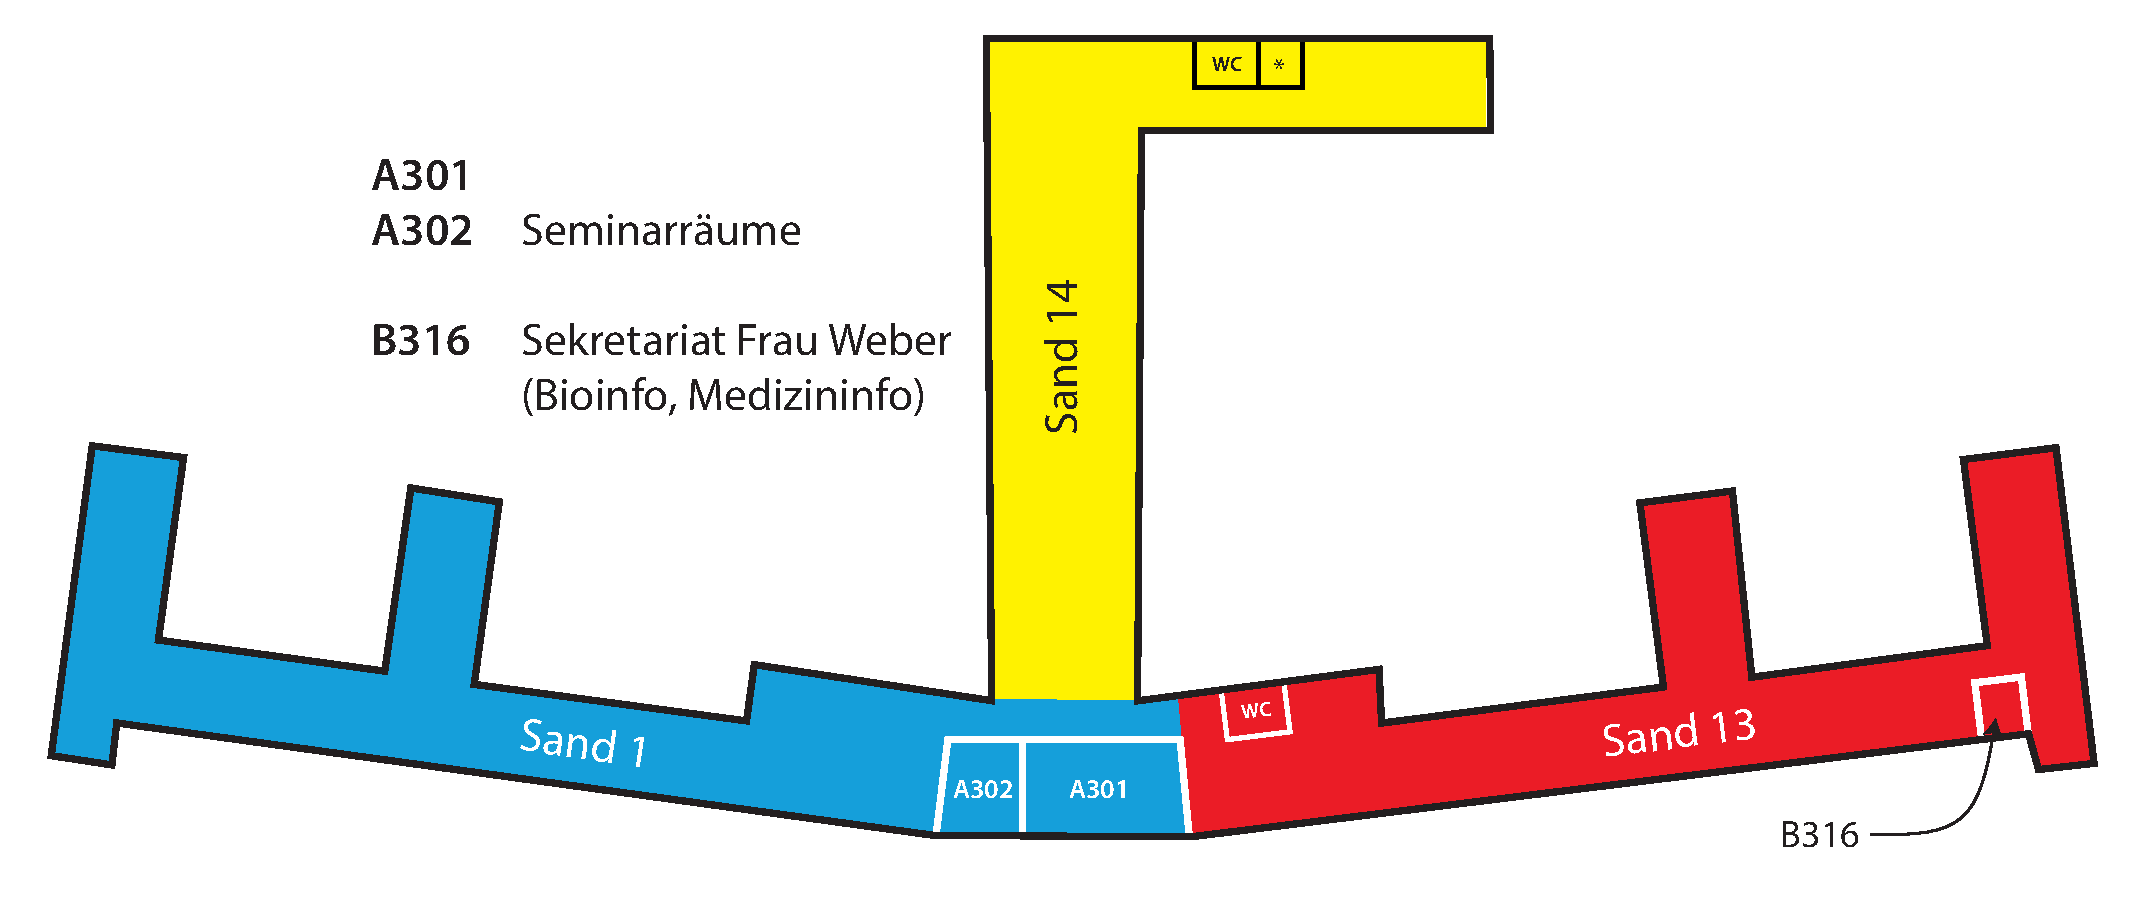
\includegraphics[width=\textwidth]{info/anhang/lageplaene/sand_2og.pdf}
\end{figure}
\else
	Tübingen hat keine Universität, Tübingen ist eine Universität. Daher existiert auch kein Uni-Campus im herkömmlichen Sinne, alles spielt sich irgendwo in der Stadt ab.
In eurem ersten Semester werdet ihr vor allem Vorlesung auf der Morgenstelle, im Kupferbau und im Psychologischen Institut haben. Für die letzten beiden haben wir leider noch keine Gebäudepläne, die wir hier abdrucken können.\\
In den höheren Semestern werdet ihr auch immer mal wieder Veranstaltungen auf dem Sand haben. Damit ihr euch dort zurechtfindet, haben wir hier ein paar Lagepläne zusammengefasst. Diese sind keinesfalls allumfassend, sie sollen euch lediglich eine grobe Orientierung durch den Dschungel der Uni-Gebäude bieten.
\subsection*{Morgenstelle}
\begin{figure}[ht!]
\centering
\includegraphics[width=0.5\textwidth]{kogni/anhang/lageplaene/uebersicht_morgenstelle.pdf}
\end{figure}
\newpage
\subsection*{Sand}
\begin{figure}[ht!]
	\centering
	\includegraphics[width=0.8\textwidth]{kogni/anhang/lageplaene/uebersicht_sand.pdf}
\end{figure}
\subsection*{Psychologisches Institut}
\begin{figure}[ht!]
	\centering
	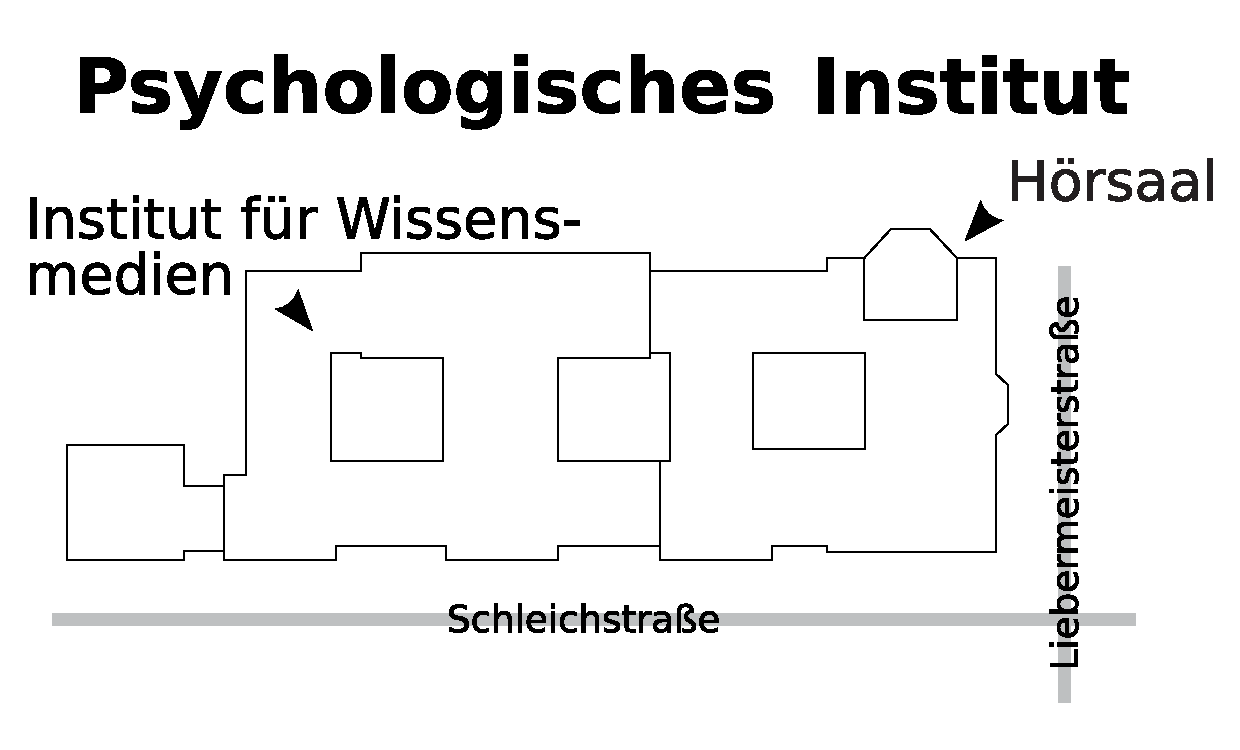
\includegraphics[width=\textwidth]{kogni/anhang/lageplaene/uebersicht_pi.pdf}
\end{figure}
%\newpage
%\subsubsection*{Sand, Erdgeschoss}~
%\begin{figure}[ht!]
%	\centering
%	\includegraphics[width=0.8\textwidth]{anhang/lageplaene/sand_eg.pdf}
%\end{figure}
%\newpage 
%\subsubsection*{Sand, 1. OG}~
%\begin{figure}[ht!]
%	\centering
%	\includegraphics[width=0.8\textwidth]{anhang/lageplaene/sand_1og.pdf}
%\end{figure}
%\subsubsection*{Sand, 2. OG}~
%\begin{figure}[ht!]
%	\centering
%	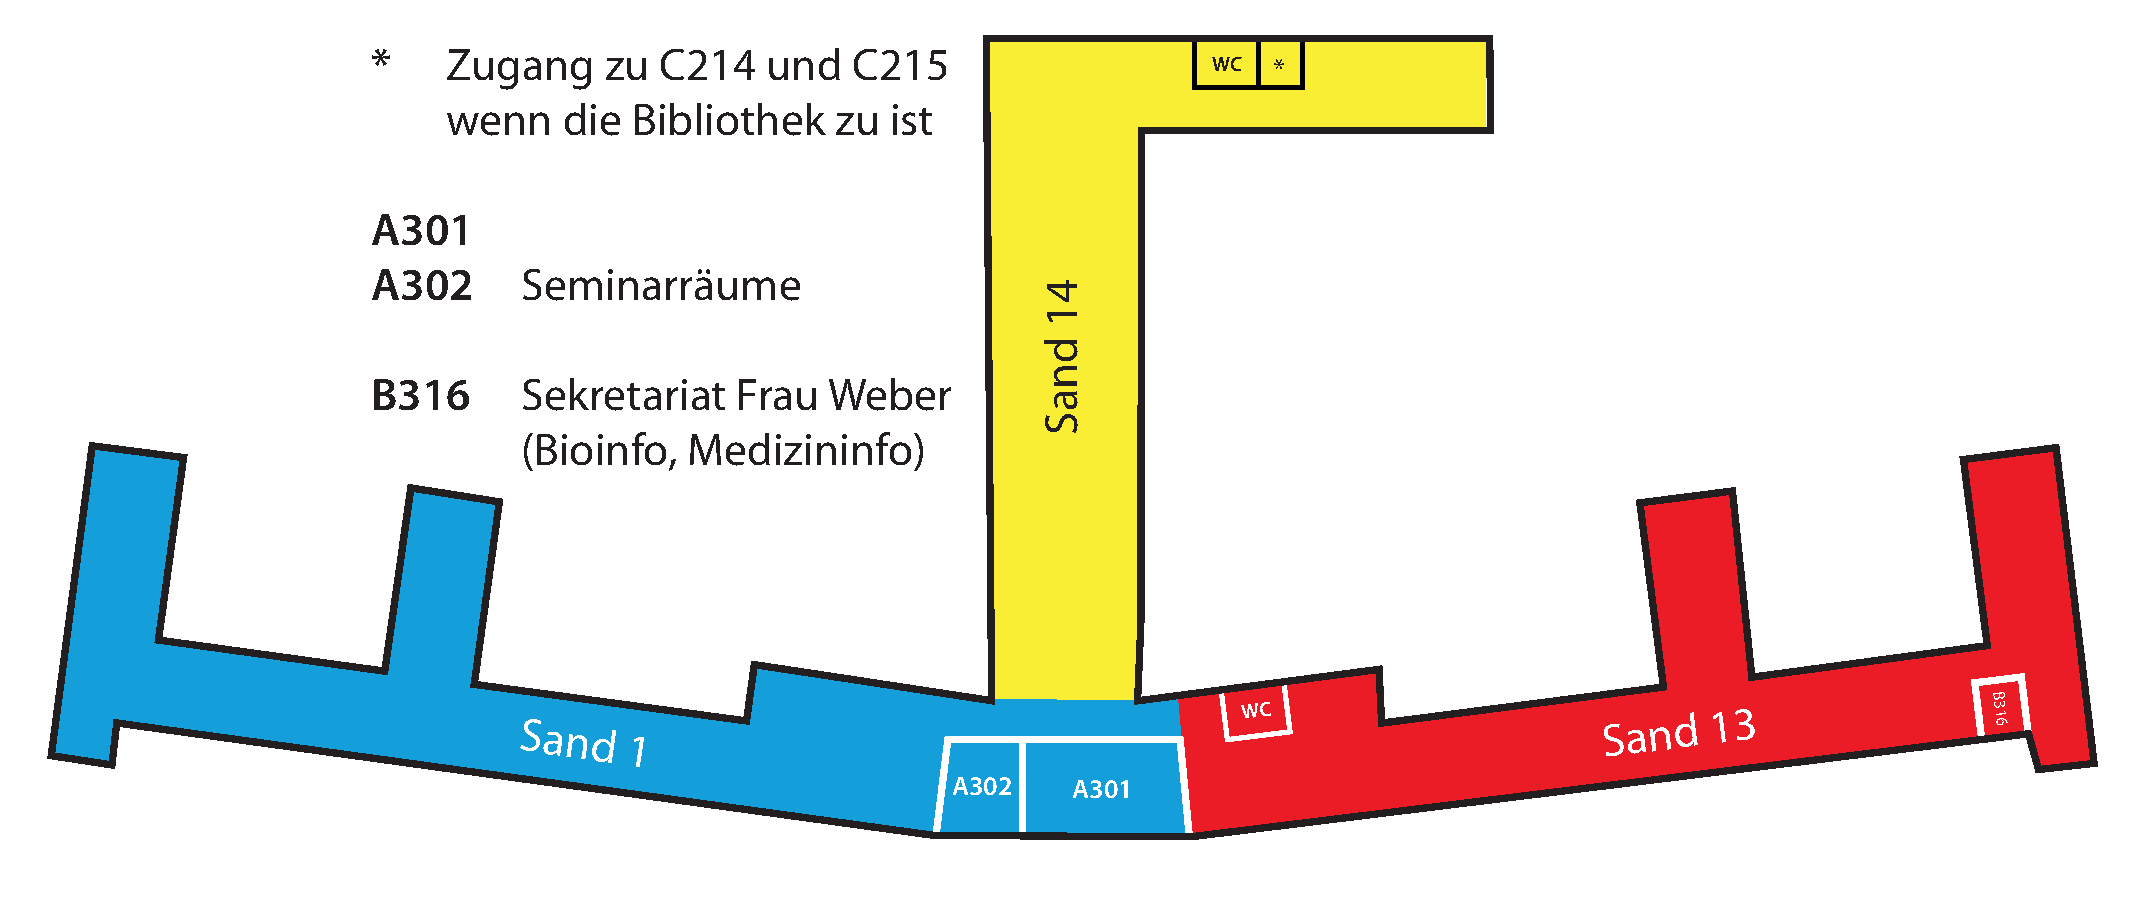
\includegraphics[width=\textwidth]{anhang/lageplaene/sand_2og.pdf}
%\end{figure}
\fi
\newpage


%\pagebreak
\section*{Verz. wicht. Abk.}
%\section*{Verz. wicht. Abk.}
\renewcommand{\arraystretch}{1.2}
\begin{tabular}{ll}
BaföG    & Bundesausbildungsförderungsgesetz \\
B.Ed.	 & Bachelor of Education (Lehramt) \\
B.Sc.    & Bachelor of Science \\
CHF      & Clubhausfest \\
c.t.     & Lat.: cum tempore (15 Minuten später) \\
ECTS     & European Credit Transfer System \\
FB       & Fachbereich \\
FH       & Fachhochschule (Reutlingen) \\
fsi      & Fachschaft Informatik \\
fsk      & Fachschaft Kognitionswissenschaften \\
FS(R)VV  & Fachschaften-(Räte-)Vollversammlung \\
HDLZ     & Hausmeister-Dienstleistungszentrum \\
HSZ      & Hörsaalzentrum \\
LP       & Leistungspunkte (auch: ECTS-Punkte) \\
M.Sc.    & Master of Science \\
naldo    & Neckar-Alb-Donaukreis\\
NF       & Nebenfach \\
o.B.d.A. & Ohne Beschränkung der Allgemeinheit \\
PA       & Prüfungsausschuss \\
PI       & Psychologisches Institut \\
RTFM     & Read the fucking manual \\
SNAFU    & Situation normal, all fucked up \\
SQ       & Schlüsselqualifikation, veraltet für übK\\
s.t.     & Lat.: sine tempore (pünktlicher Beginn) \\
StuRa    & Studierendenrat \\
StuWe    & Studierendenwerk \\
SWT      & Stadtwerke Tübingen \\
übK      & überfachliche berufsfeldorientierte Kompetenzen \\
UB       & Universitätsbibliothek (Wilhelmstraße) \\
WHO      & Waldhäuser Ost \\
WSI      & Wilhelm-Schickard-Institut für Informatik \\
ZDV      & Zentrum für Datenverarbeitung \\
ZV       & Zentrale Verwaltung\\
\end{tabular}
\vfill %\pagebreak

\ifinfo
	\pagebreak
\fi


% Placeholder-Seite für Seitenzahl

%\pagebreak
\addcontentsline{toc}{section}{Stundenplan zum selbst ausfüllen}
\begin{center}
	\begin{sidewaysfigure}
		\renewcommand{\arraystretch}{2.8}
\begin{footnotesize}
\begin{tabular}{|l|p{0.15\textwidth}|p{0.15\textwidth}|p{0.15\textwidth}|p{0.15\textwidth}|p{0.15\textwidth}|} \hline
			Zeit      & 			Montag 		& Dienstag		& Mittwoch 			& Donnerstag  	& Freitag 	\\ \hline \hline 
			08 -- 09  &							&				&					&				&			\\ 	
			09 -- 10  &							&				&					&				&			\\ \hline
			10 -- 11  &							&				&					&				&			\\ 	
			11 -- 12  &							&				&					&				&			\\ \hline
			12 -- 13  &							&				&					&				&			\\ 	
			13 -- 14  &							&				&					&				&			\\ \hline
			14 -- 15  &							&				&					&				&			\\ 	
			15 -- 16  &							&				&					&				&			\\ \hline
			16 -- 17  &							&				&					&				&			\\ 	
			17 -- 18  &							&				&					&				&			\\ \hline
			18 -- 19  &							&				&					&				&			\\ 	
			19 -- 20  &							&				&					&				&			\\ \hline		
		\end{tabular}
		\hspace*{13cm}Donnerstags ist Clubhausfest!
\end{footnotesize}

	\end{sidewaysfigure}
\end{center}
\pagebreak
\section*{Platz für Notizen:}
\ifinfo
	\newpage\null\thispagestyle{empty}\newpage
\fi

\addcontentsline{toc}{section}{Adressen \& Telefonnummern}
\ifinfo
	\textbf{Unsere Professoren:}\\\\
\link{https://uni-tuebingen.de/de/14097}{%
  Alle Infos zu den Professoren findet ihr der Website des Fachbereichs Informatik}

\begin{tabular}{ll}
Prüfungsausschussvorsitz: & \PAVorsitz \\
Studiendekan:             & \Studiendekan\\
Fachbereichssprecher:     & \FBSprecher\\
Stellv. FB Sprecher:      & \StellvFBSprecher\\
\end{tabular}

\textbf{Studienberatung:}\\\\
\link{https://uni-tuebingen.de/de/74360}{%
  Für Beratung während des Studiums könnt ihr hier nochmal alle wichtigen Kontakte finden}

\vfill
\normalsize

\else
	%%damit adressen auf gerader seitenzahl sind
	\pagebreak
	\renewcommand{\arraystretch}{1}
\normalsize 
\textbf{Unsere Professoren:}\\\\
\footnotesize

\begin{tabular}{|p{0.25\textwidth}p{0.45\textwidth}p{0.2\textwidth}|}
\hline
Name                          & Arbeitsbereich & Funktionen \\
\hline
\hline
Prof. Harald Baayen			& Quantitative Linguistik 				& \\
Prof. Martin Butz           & Kognitive Modellierung 				& Studiendekan	\\
Prof. Volker Franz			& Experimentelle Kognitionswissenschaft	& \\
Prof. Thorsten Grust		& Datenbanksysteme & \\
Prof. Matthias Hein			& Maschinelles Lernen & \\
Prof. Hanspeter Mallot 		& Kognitive Neurowissenschaft	& \\
Prof. Bettina Rolke			& Evolutionäre Kognition	& \\
Prof. Rolf Ulrich			& Wahrnehmung und Kognition	& \\
Prof. Felix Wichmann        & Neuronale Informationsverarbeitung	& PA Vorsitzender\\
Prof. Andreas Zell          & Kognitive Systeme 		 &\\
Prof. Hendrik Lensch & Computergrafik &\\
Prof. Thomas Markwig & Mathematik &\\
Dr. Britta Dorn & Mathematische Strukturen in der Informatik &\\
\hline
\end{tabular}
%\enlargethispage{4ex}

\scriptsize{PA = Prüfungsausschuss}

\vspace{1cm}
\normalsize 
\textbf{Wichtige Personen:}\\\\
\footnotesize
\begin{tabular}{|p{3cm} p{7.5cm} p{4cm}|}
\hline
Name                  & Adresse & Tätigkeit \hfill \\
\hline
\hline
Violaine Le Guily\newline Dr. Elisabeth Hein & Schleichstraße 4.  Ebene 2, Zimmer 4240\newline\email{studienberatung@kogwis.uni-tuebingen.de} & Koordination für Studium und Lehre,\newline Studienberatung\\
\hline
\studBeratungTwolines & \email{kogni-beratung@fsi.uni-tuebingen.de} & Studentische\newline Studienberatung\\
\hline
\kognimentorenTwolines & \email{kogni-mentoren@fsi.uni-tuebingen.de} & ErstsemestermentorInnen\\         
\hline
Ilona Gold	      & Keplerstr. 2, Raum 206.1\newline \email{pruefungsamt.kognitionswissenschaft@uni-tuebingen.de} & Prüfungssekretariat \newline Kognitionswissenschaft \\
\hline 
\end{tabular}

\fi

\ifinfo
	% Umschlagrückseite
	\thispagestyle{empty}
\vfill
\pagenumbering{gobble}
\centering

\includegraphics[height=0.7\textheight]{shared/logos/keepcalm}
\vfill 
\flushleft
%\qrcode[height=2cm]{https://www.fsi.uni-tuebingen.de/ueber-uns} \scriptsize {https://www.fsi.uni-tuebingen.de/ueber-uns}
\link{https://toot.kif.rocks/@fsi\_tue}{Folge uns im Fediverse \faIcon{mastodon}}\\
\link{https://www.fsi.uni-tuebingen.de/ueber-uns}{Wer sind wir?}

\fi

\end{document}
